% !TEX root = trkjet.tex

\part*{Auxiliary material}
\addcontentsline{toc}{part}{Auxiliary material}
%-------------------------------------------------------------------------------

%In an ATLAS paper, auxiliary plots and tables that are supposed to be made public 
%should be collected in an appendix that has the title \enquote{Auxiliary material}.
%This information will appear on the public webpage, but will not be included
%in the document submitted to arXiv and to the journal.

%
%\begin{figure}[h]
%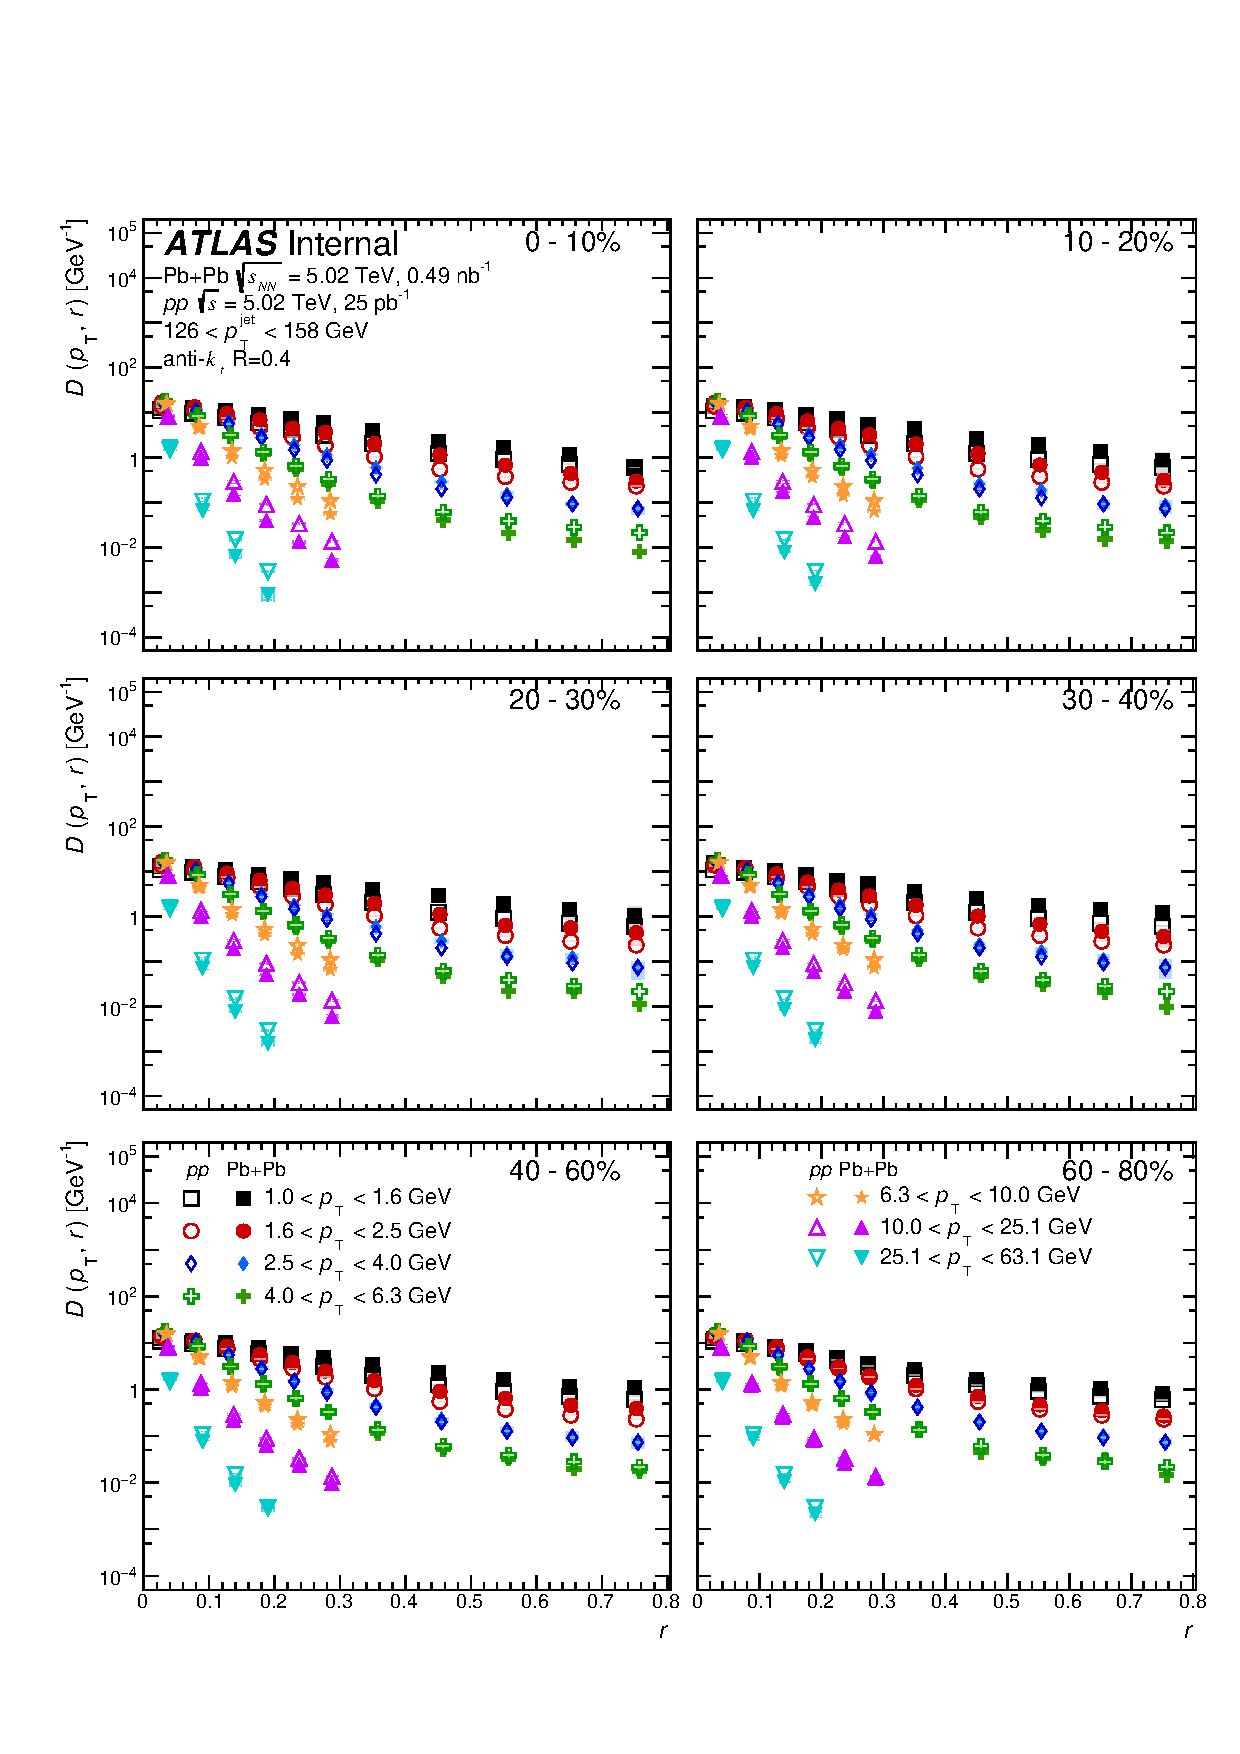
\includegraphics[width=1.0\textwidth]{figures/results/DpT_dR_jet7}
%\caption{ \Dptr\ distributions as a function of \rvar\ for different \pt\ ranges in 126--158 GeV jets.
%The open markers are for \pp\ collisions and the solid markers are for \pbpb\ collisions.
%The different panels refer to different centrality selections}
%\label{fig:fullset_dptr_j7}
%\end{figure}

\begin{figure}[h]
\centerline{
\begin{tabular}{ccc}
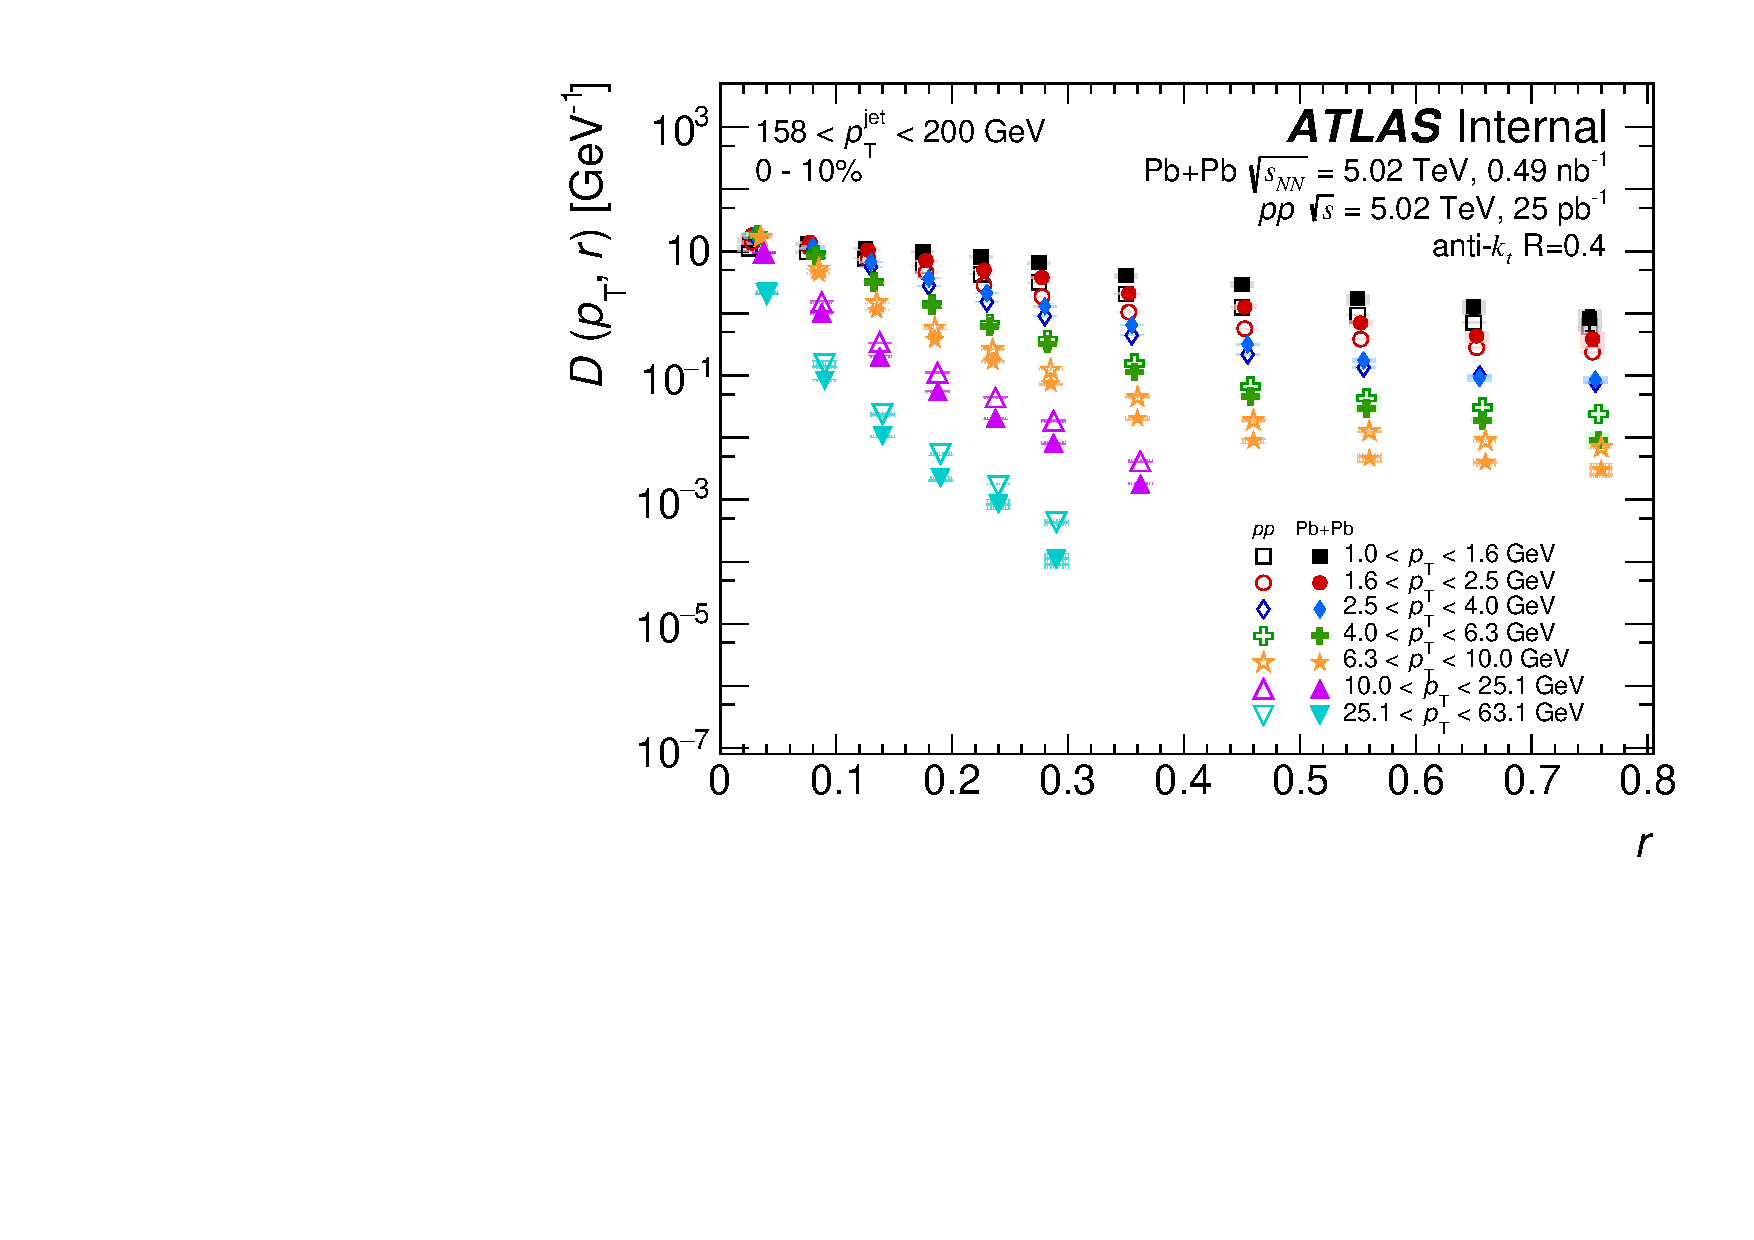
\includegraphics[width=0.48\textwidth]{figures/results/DpT_dR_jet8_cent0} &
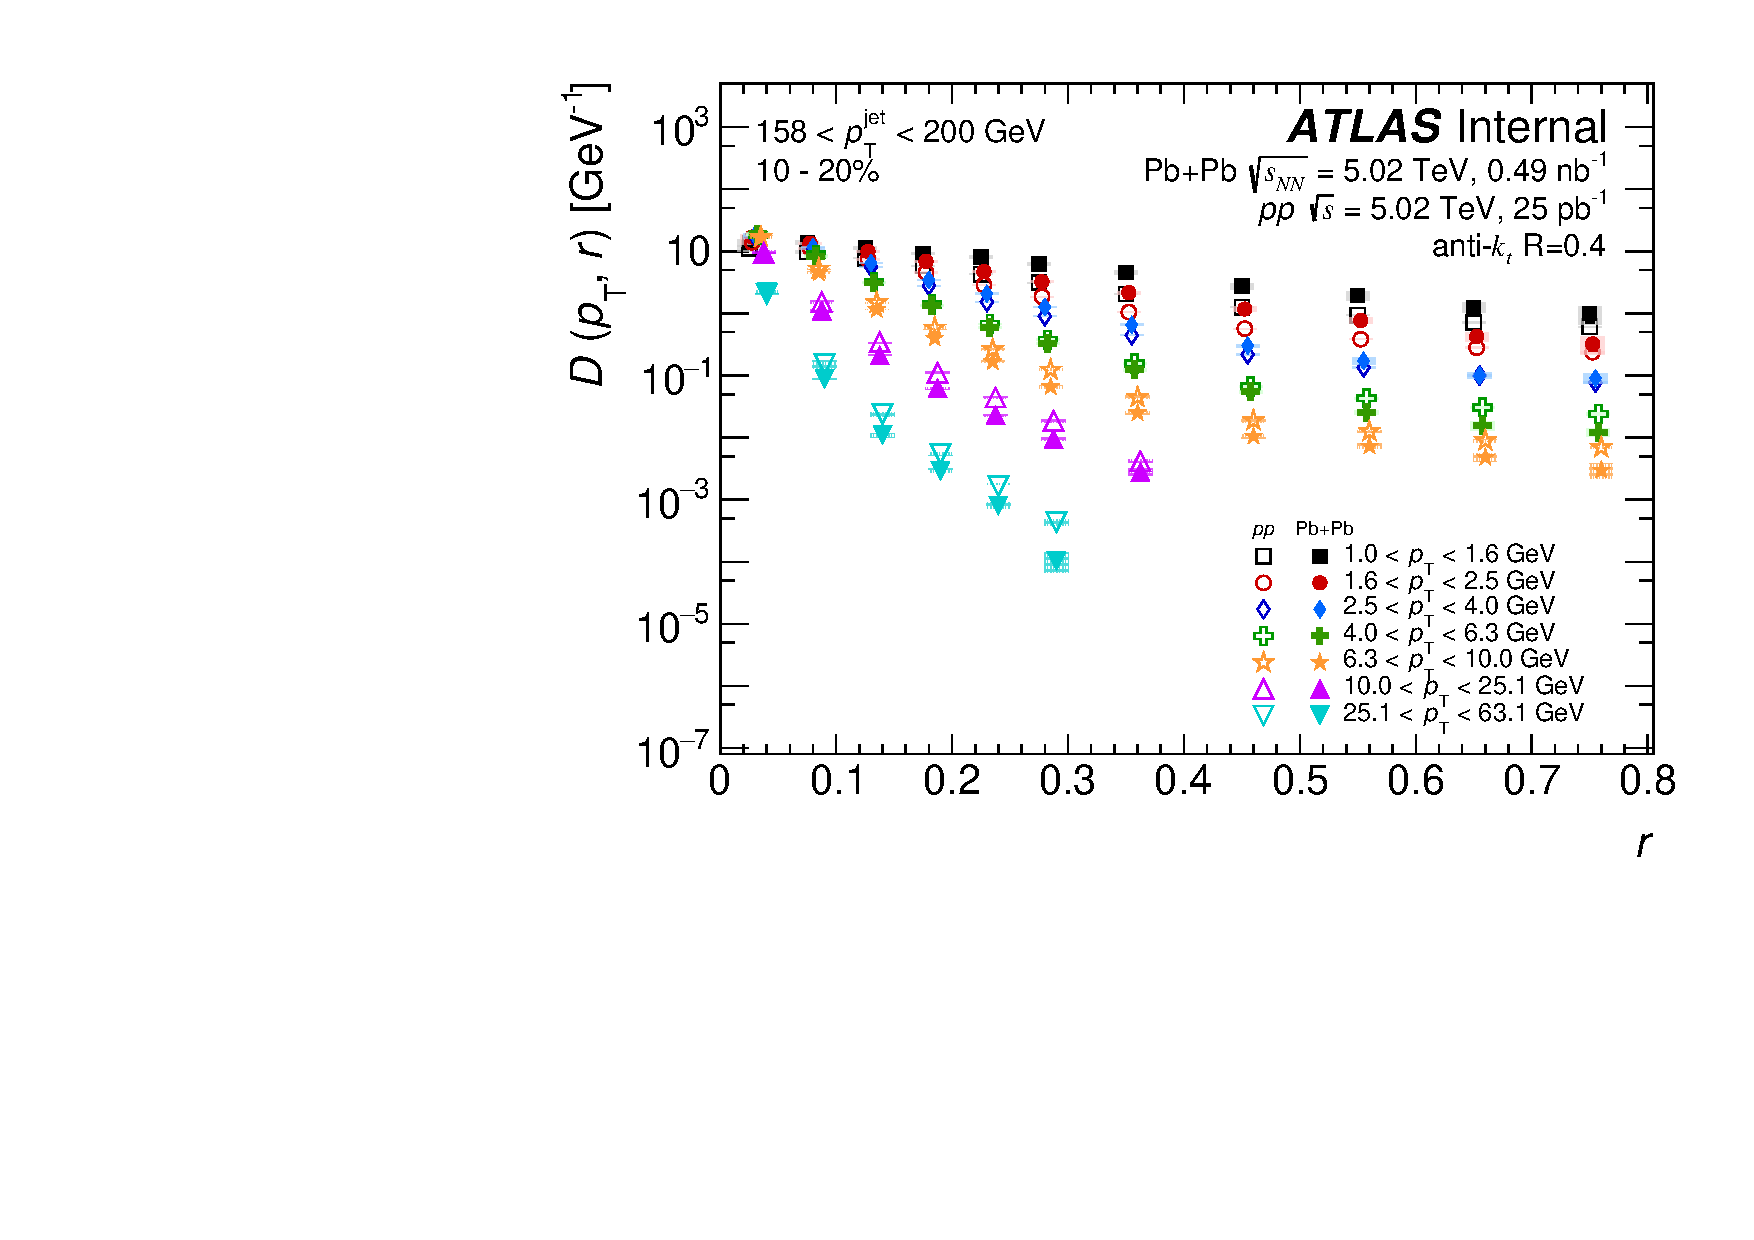
\includegraphics[width=0.48\textwidth]{figures/results/DpT_dR_jet8_cent1} \\
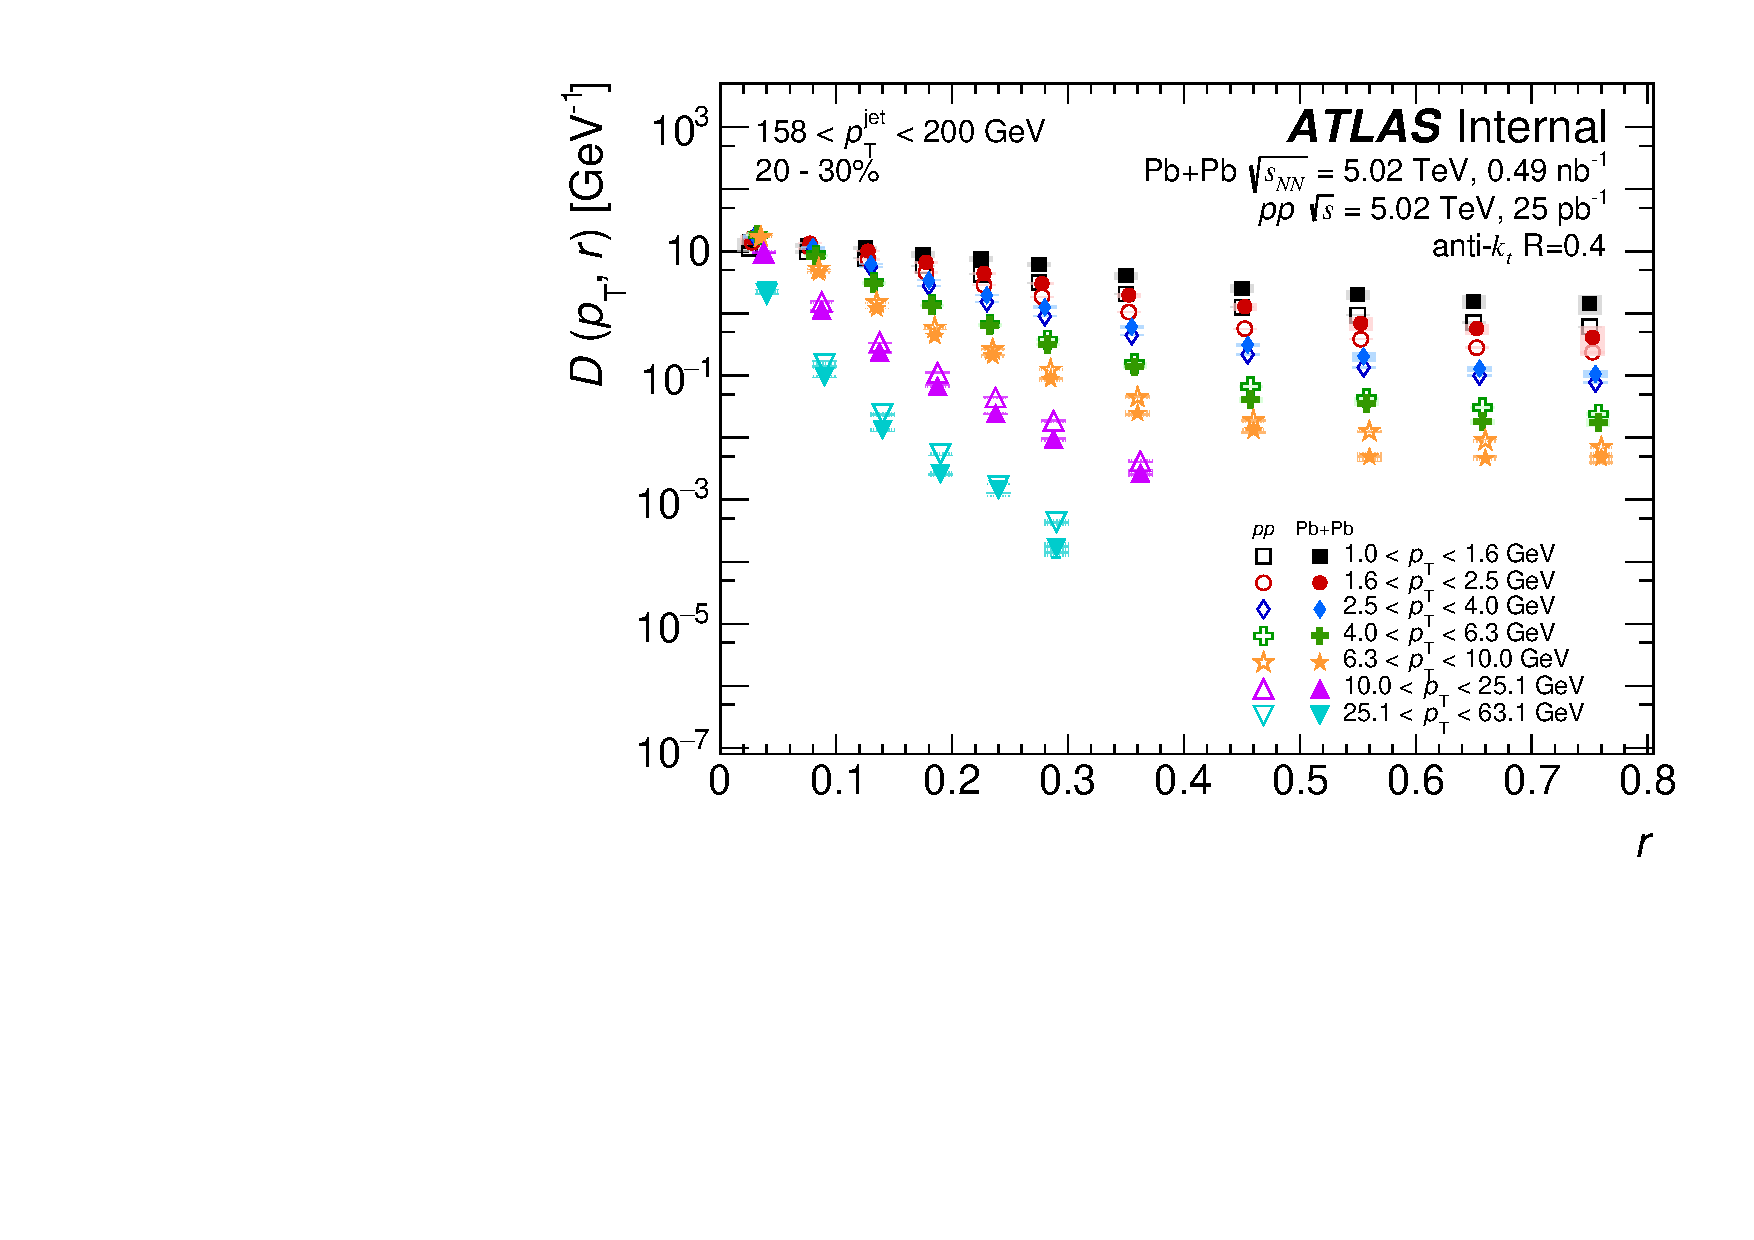
\includegraphics[width=0.48\textwidth]{figures/results/DpT_dR_jet8_cent2} &
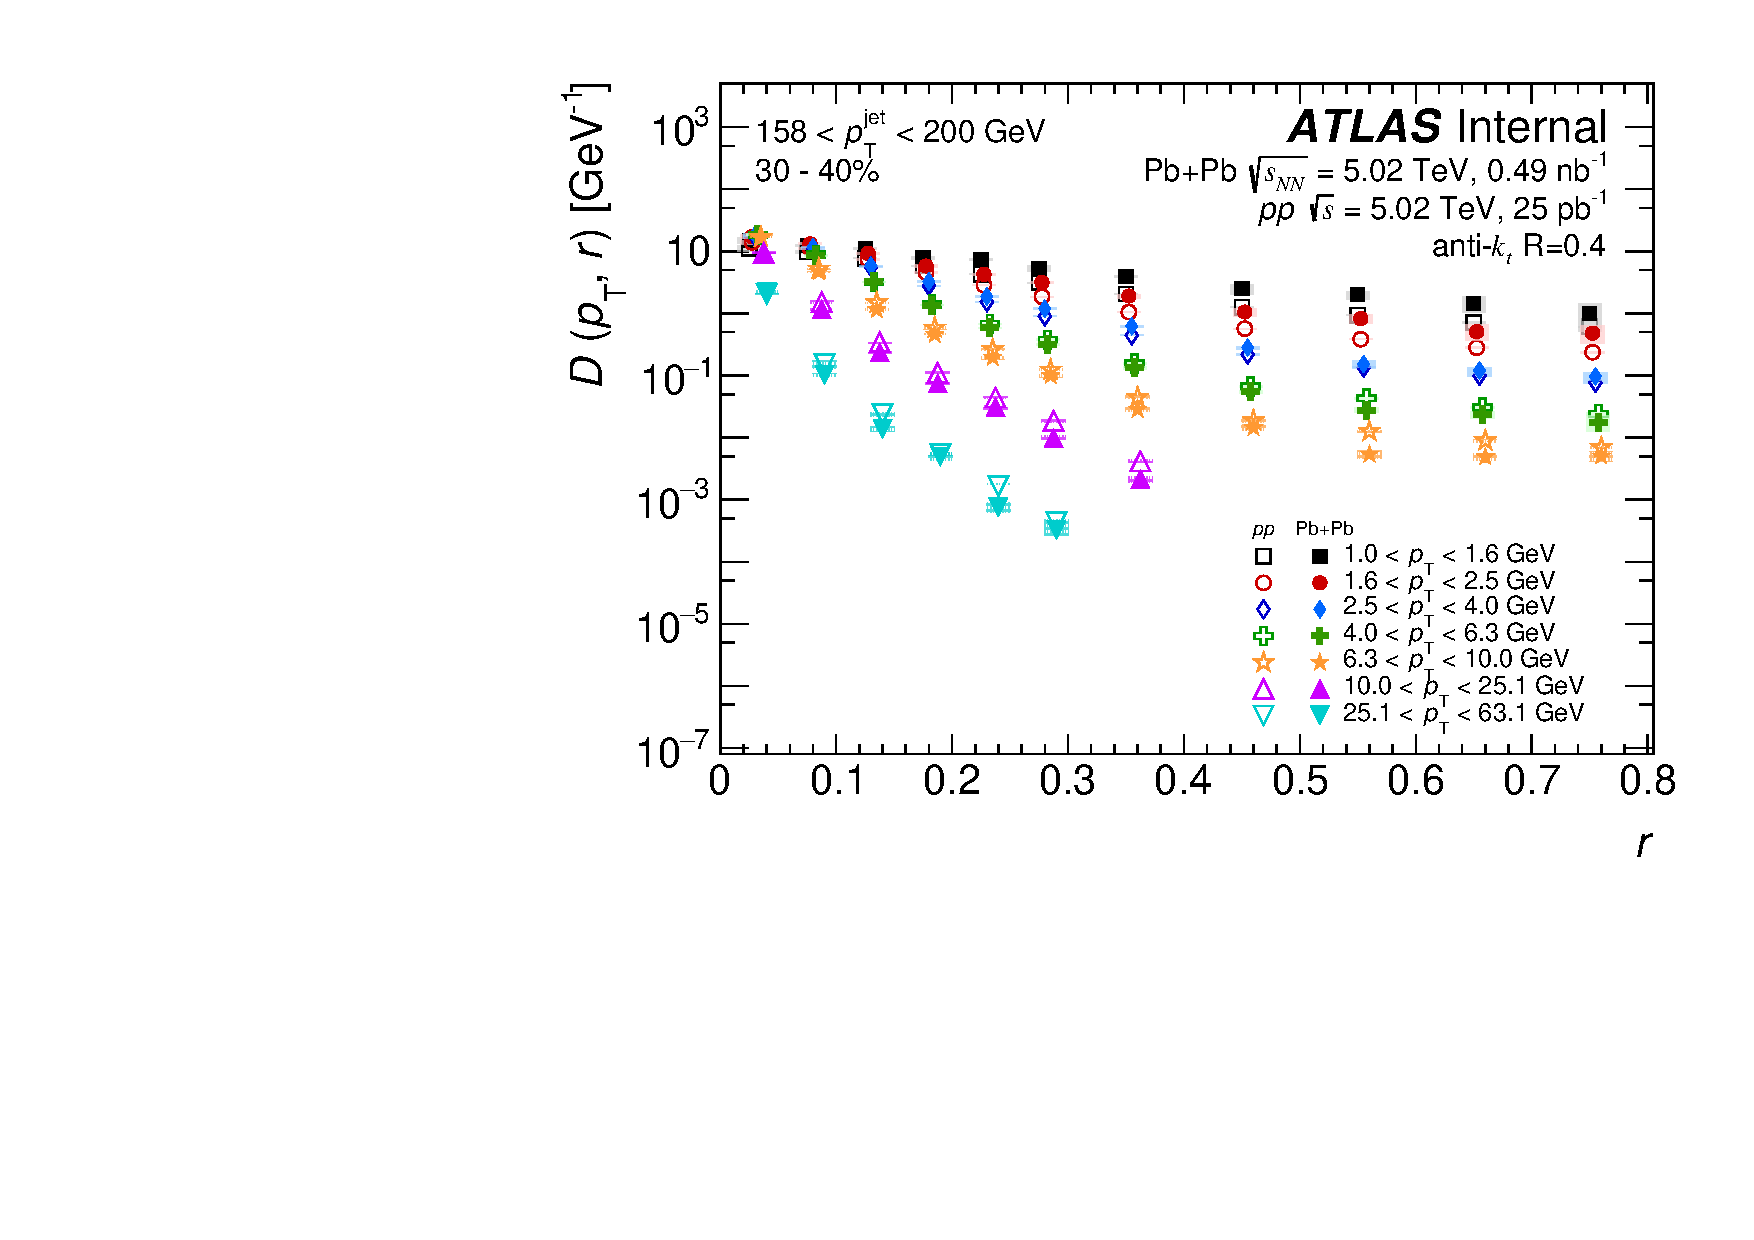
\includegraphics[width=0.48\textwidth]{figures/results/DpT_dR_jet8_cent3} \\
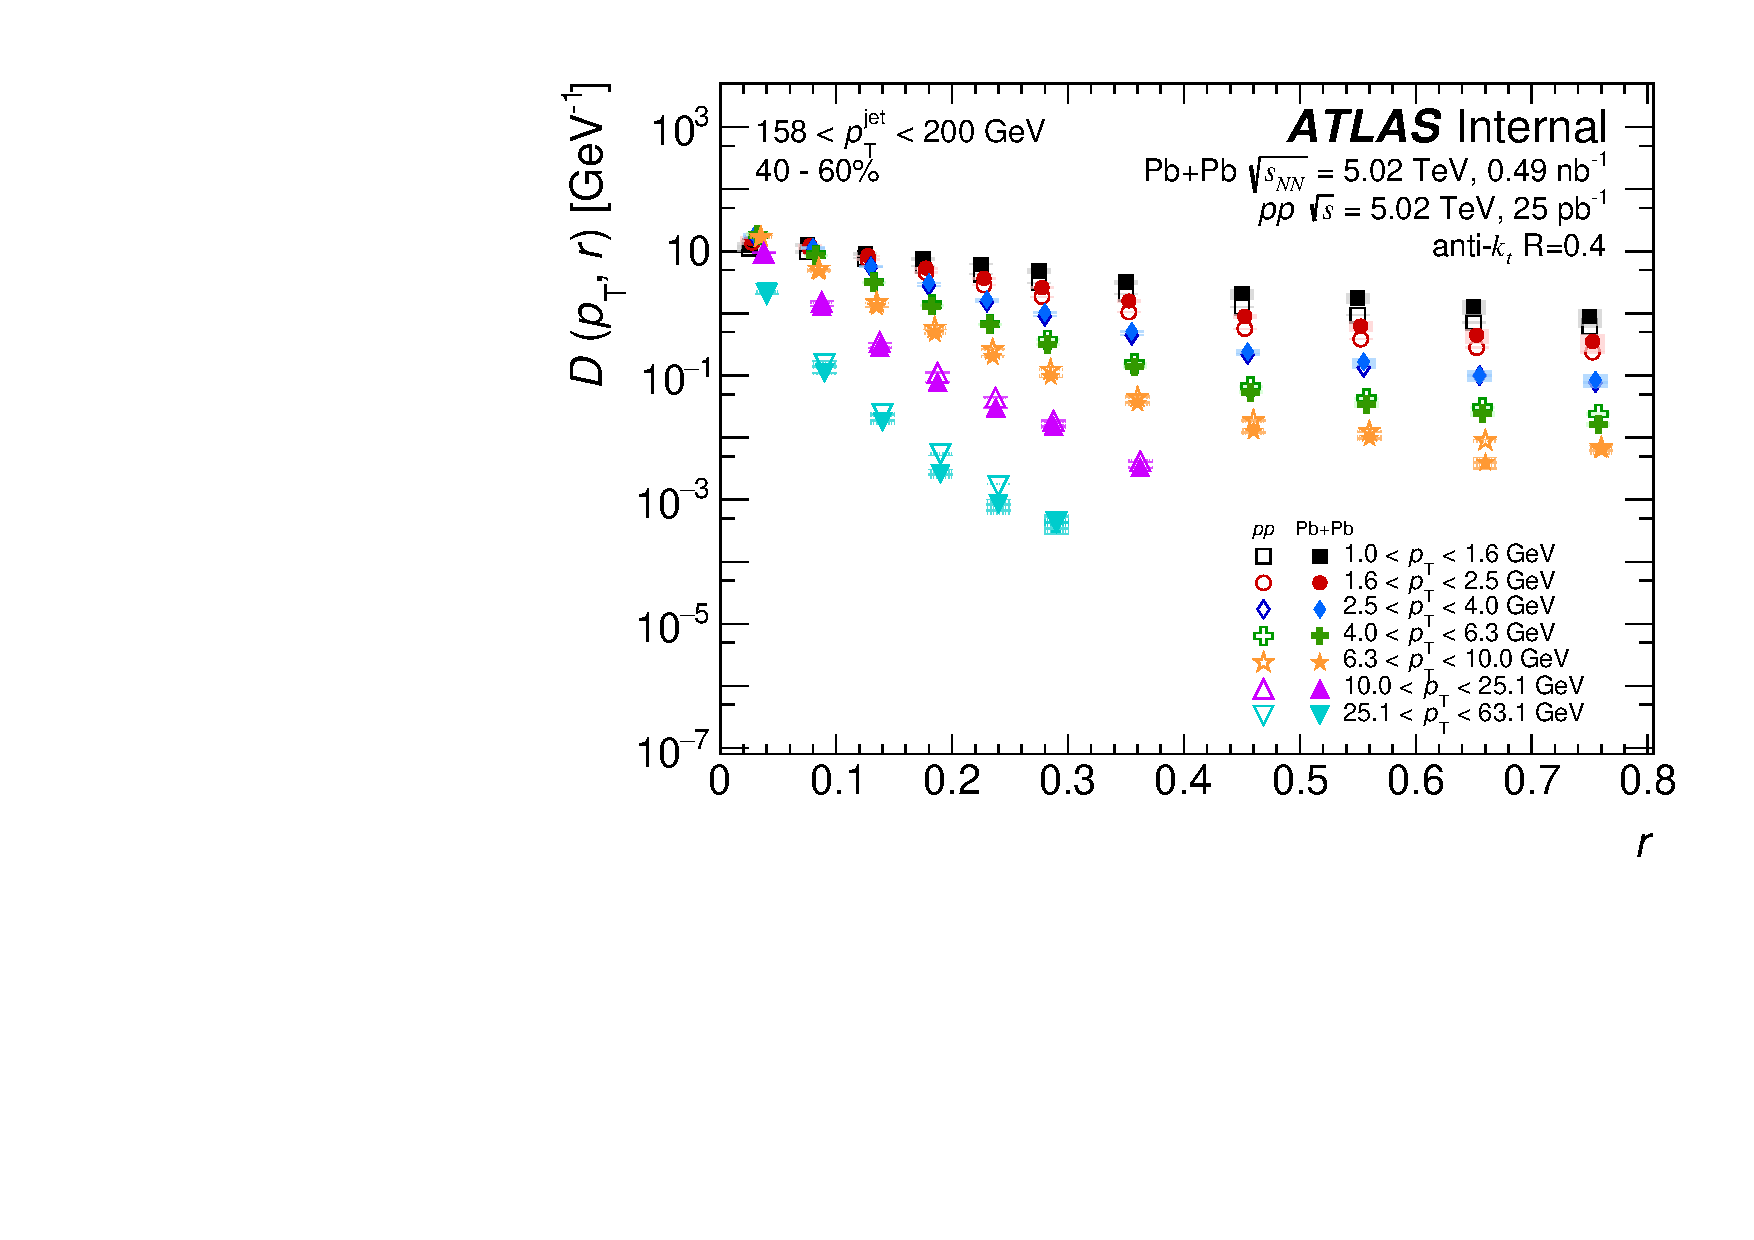
\includegraphics[width=0.48\textwidth]{figures/results/DpT_dR_jet8_cent4} &
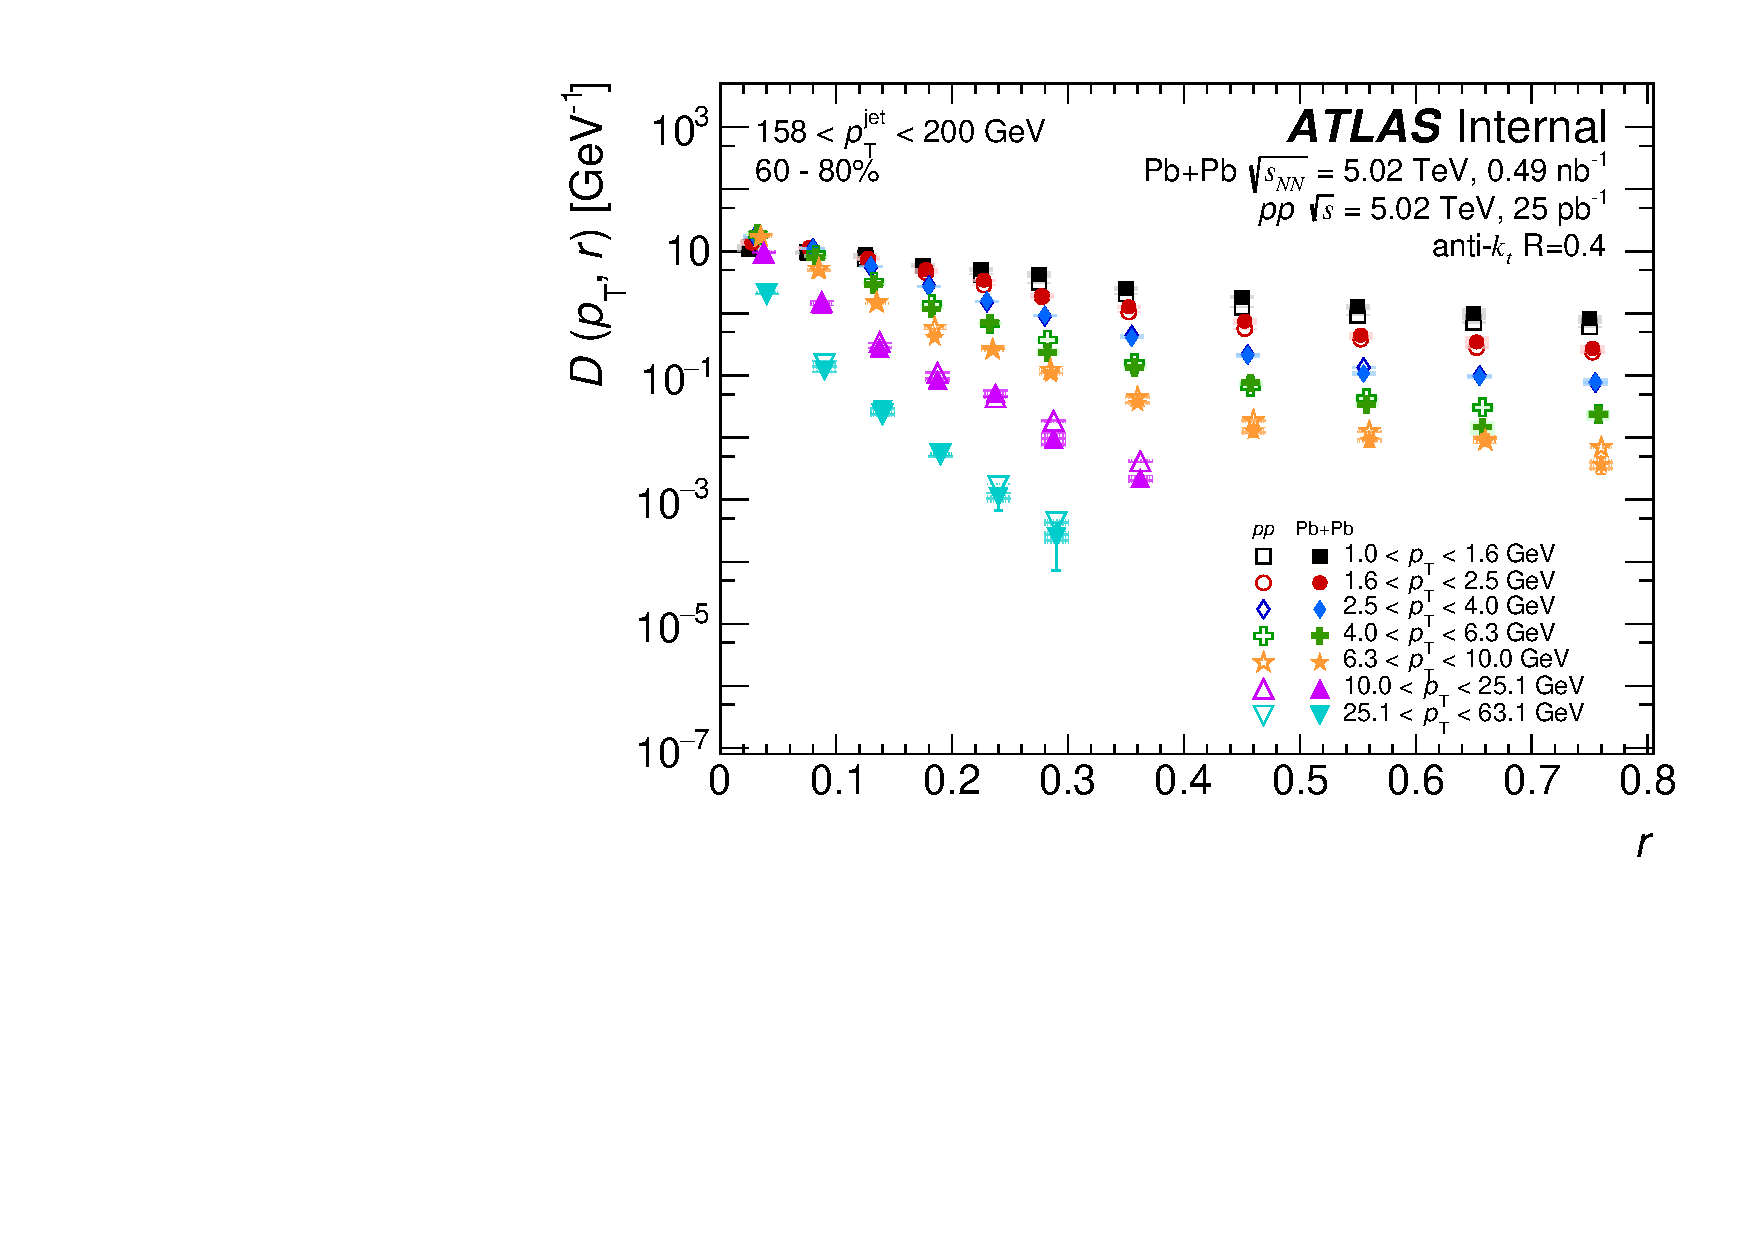
\includegraphics[width=0.48\textwidth]{figures/results/DpT_dR_jet8_cent5} \\
\end{tabular}}
\caption{ \Dptr\ distributions as a function of \rvar\ for different \pt\ ranges in 158--200 GeV jets.
The open markers are for \pp\ collisions and the solid markers are for \pbpb\ collisions.
The different panels refer to different centrality selections.
The vertical bars on the data points indicate statistical uncertainties while the shaded boxes indicate systematic uncertainties.
The widths of the boxes are not indicative of the bin size and the points are shifted horizontally for better visibility.
The distributions for $\pt > 6.3$ GeV are restricted to smaller \rvar\ values as discussed in Section~\ref{sec:analysis}.}
\label{fig:fullset_dptr_j8}
\end{figure}

\begin{figure}[h]
\centerline{
\begin{tabular}{ccc}
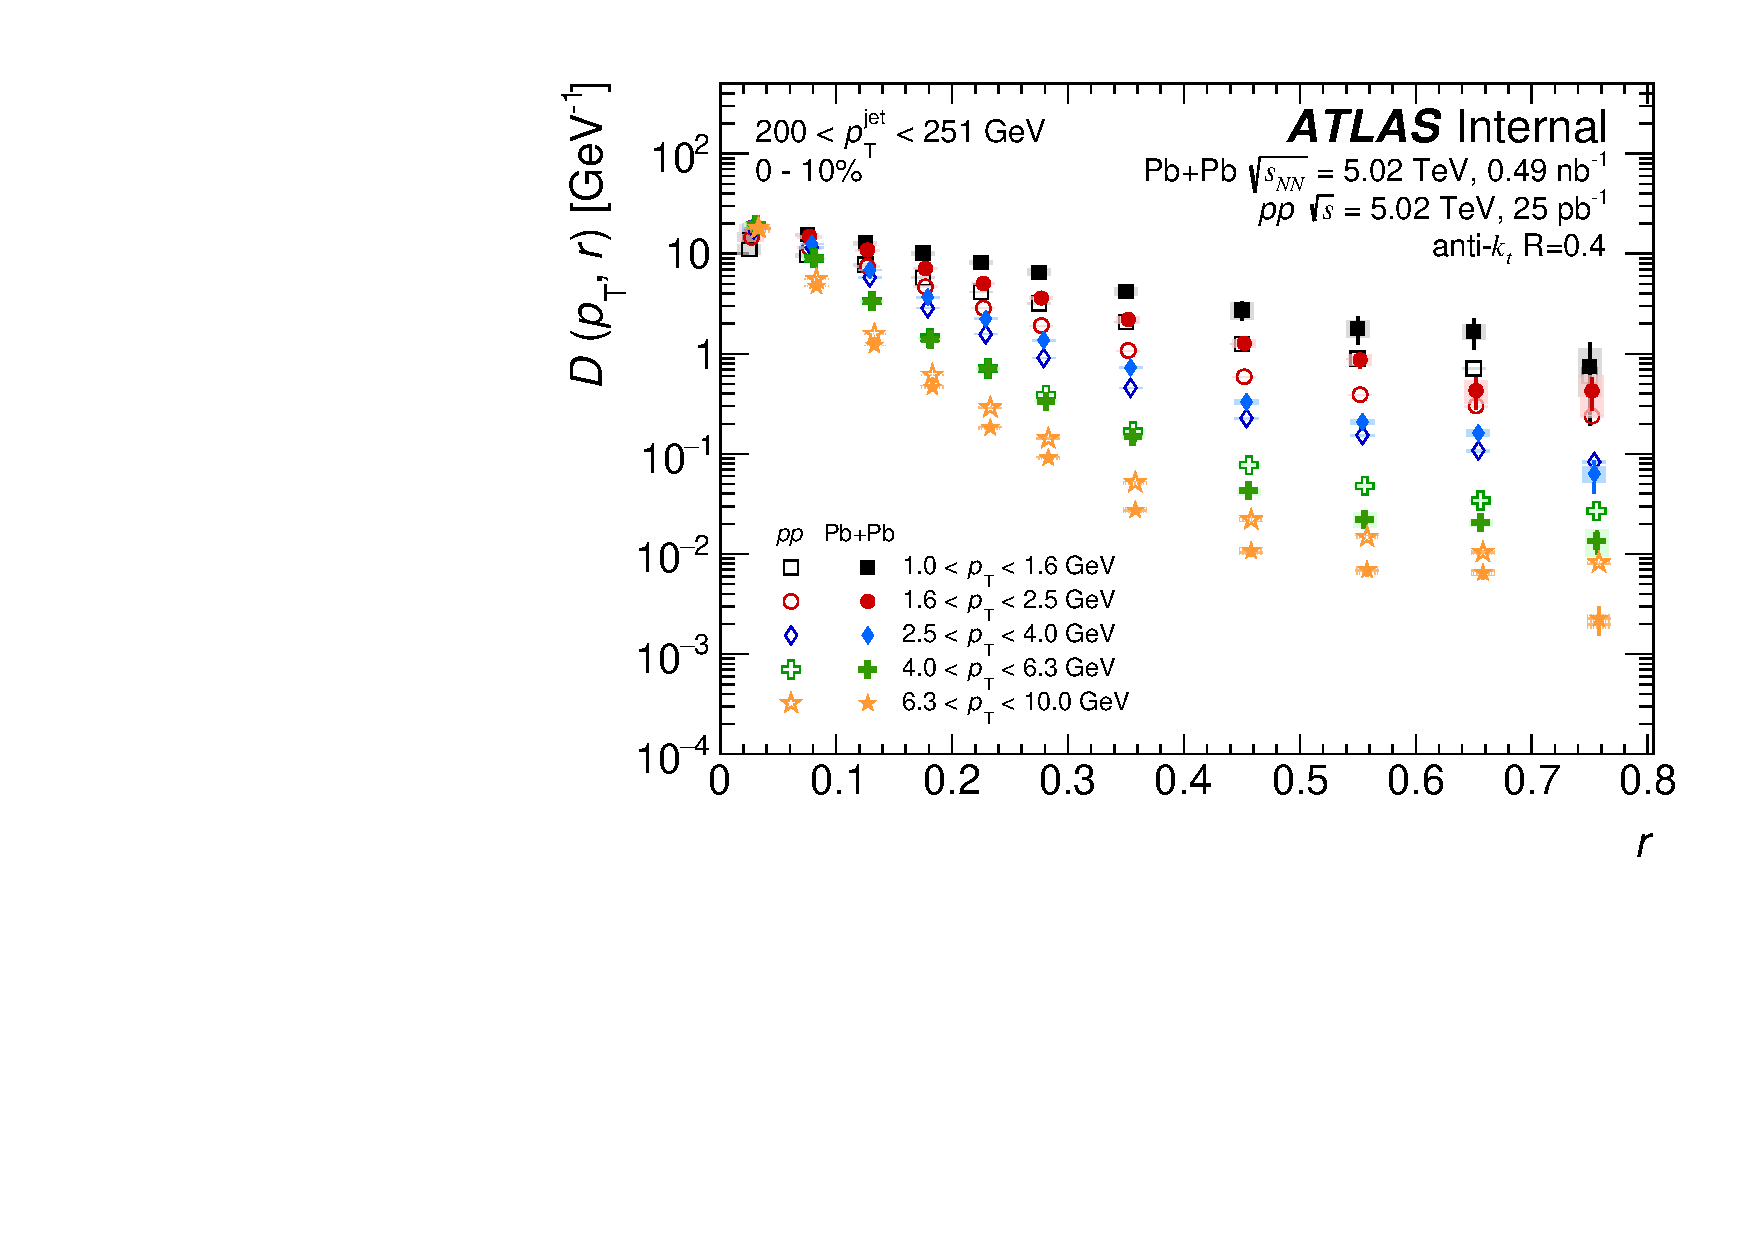
\includegraphics[width=0.48\textwidth]{figures/results/DpT_dR_jet9_cent0} &
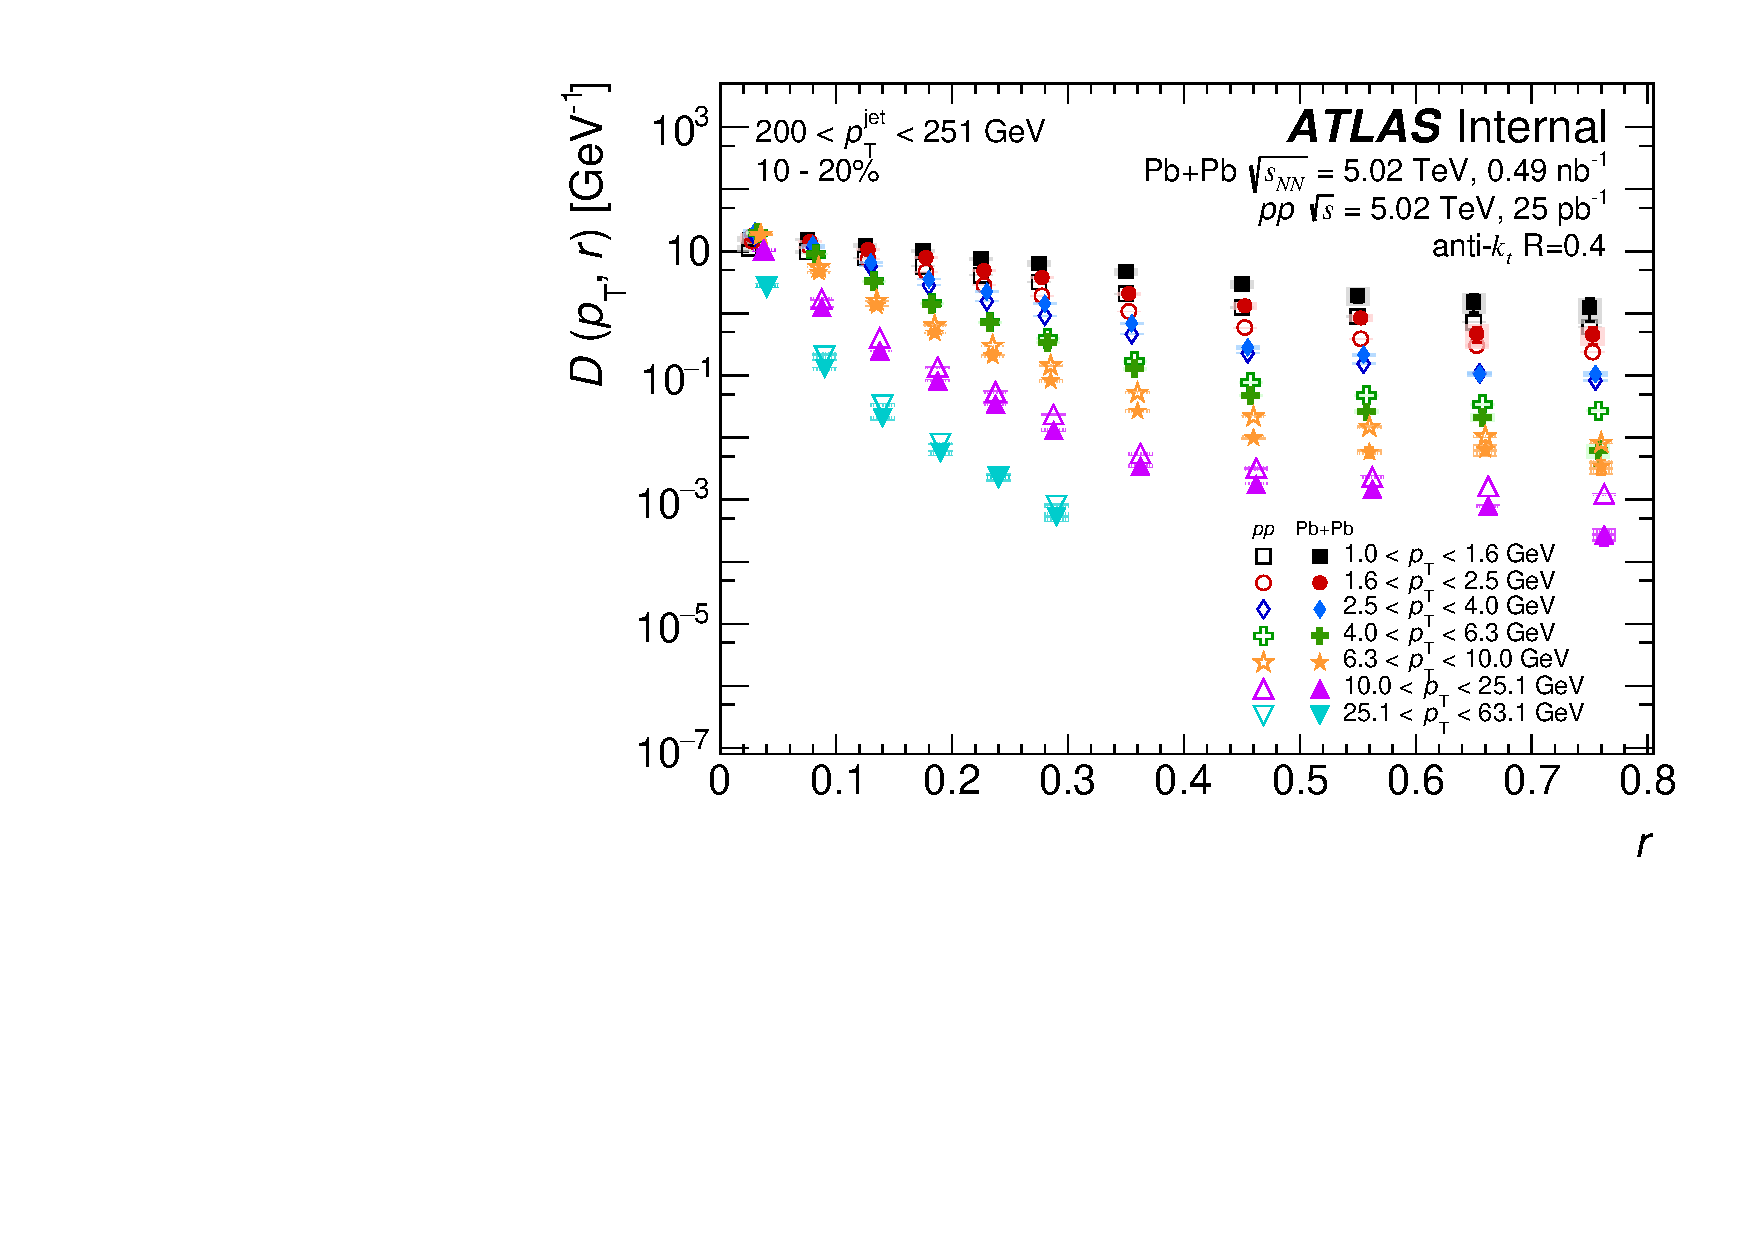
\includegraphics[width=0.48\textwidth]{figures/results/DpT_dR_jet9_cent1} \\
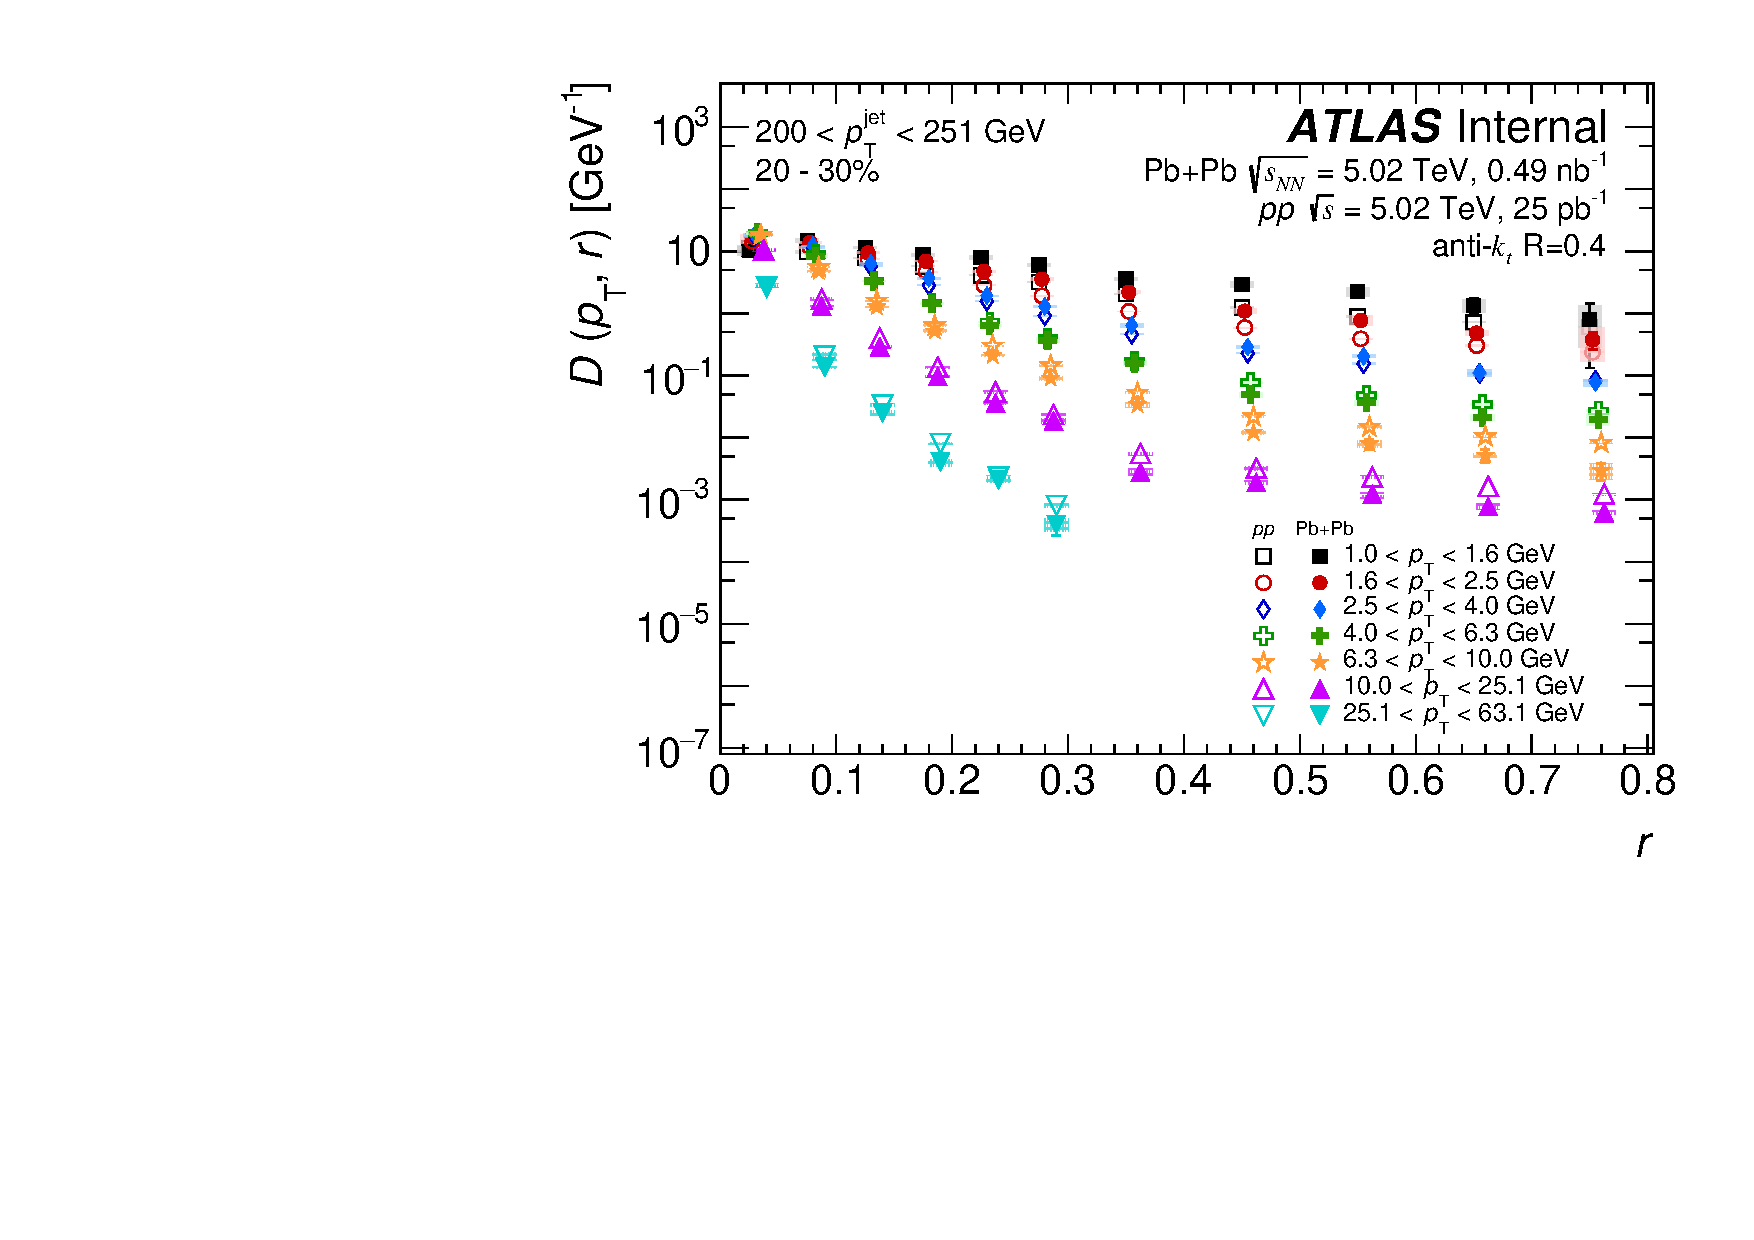
\includegraphics[width=0.48\textwidth]{figures/results/DpT_dR_jet9_cent2} &
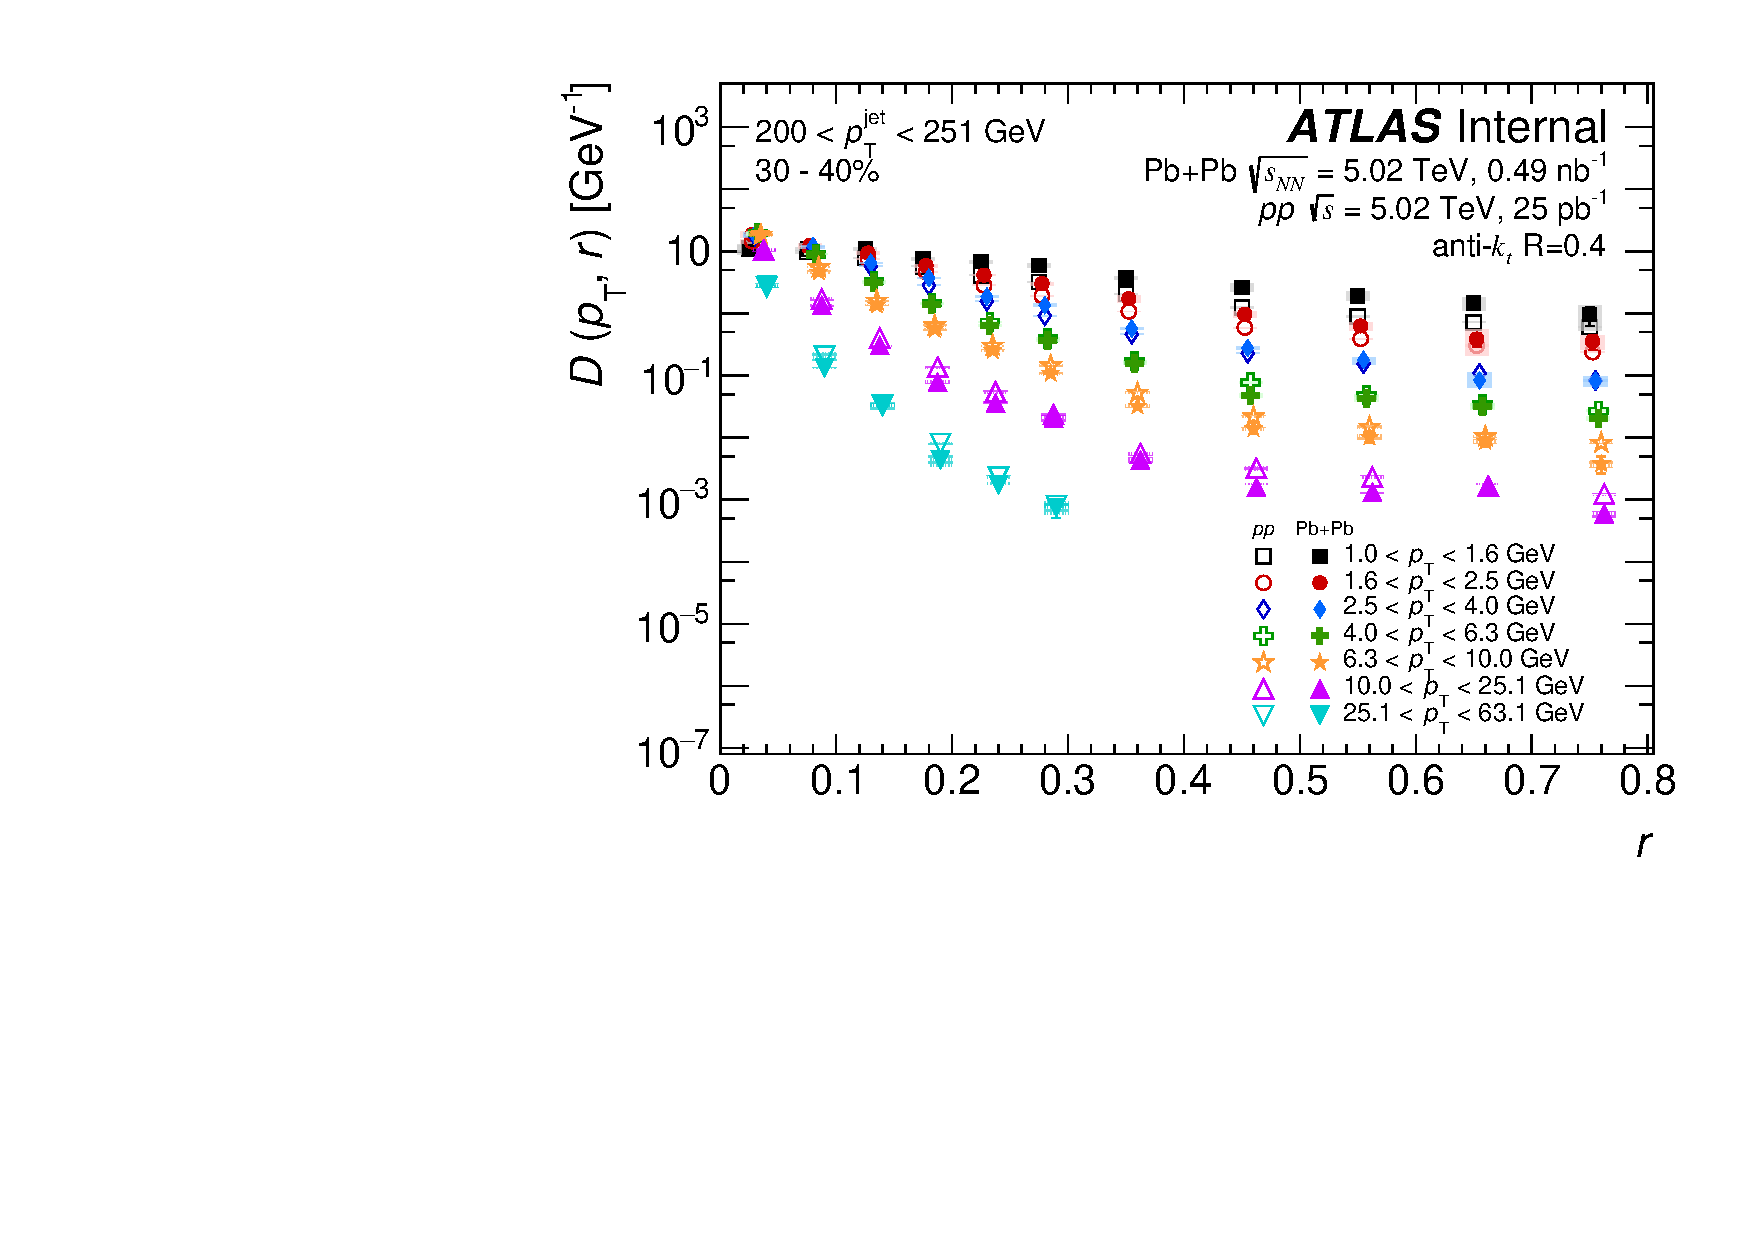
\includegraphics[width=0.48\textwidth]{figures/results/DpT_dR_jet9_cent3} \\
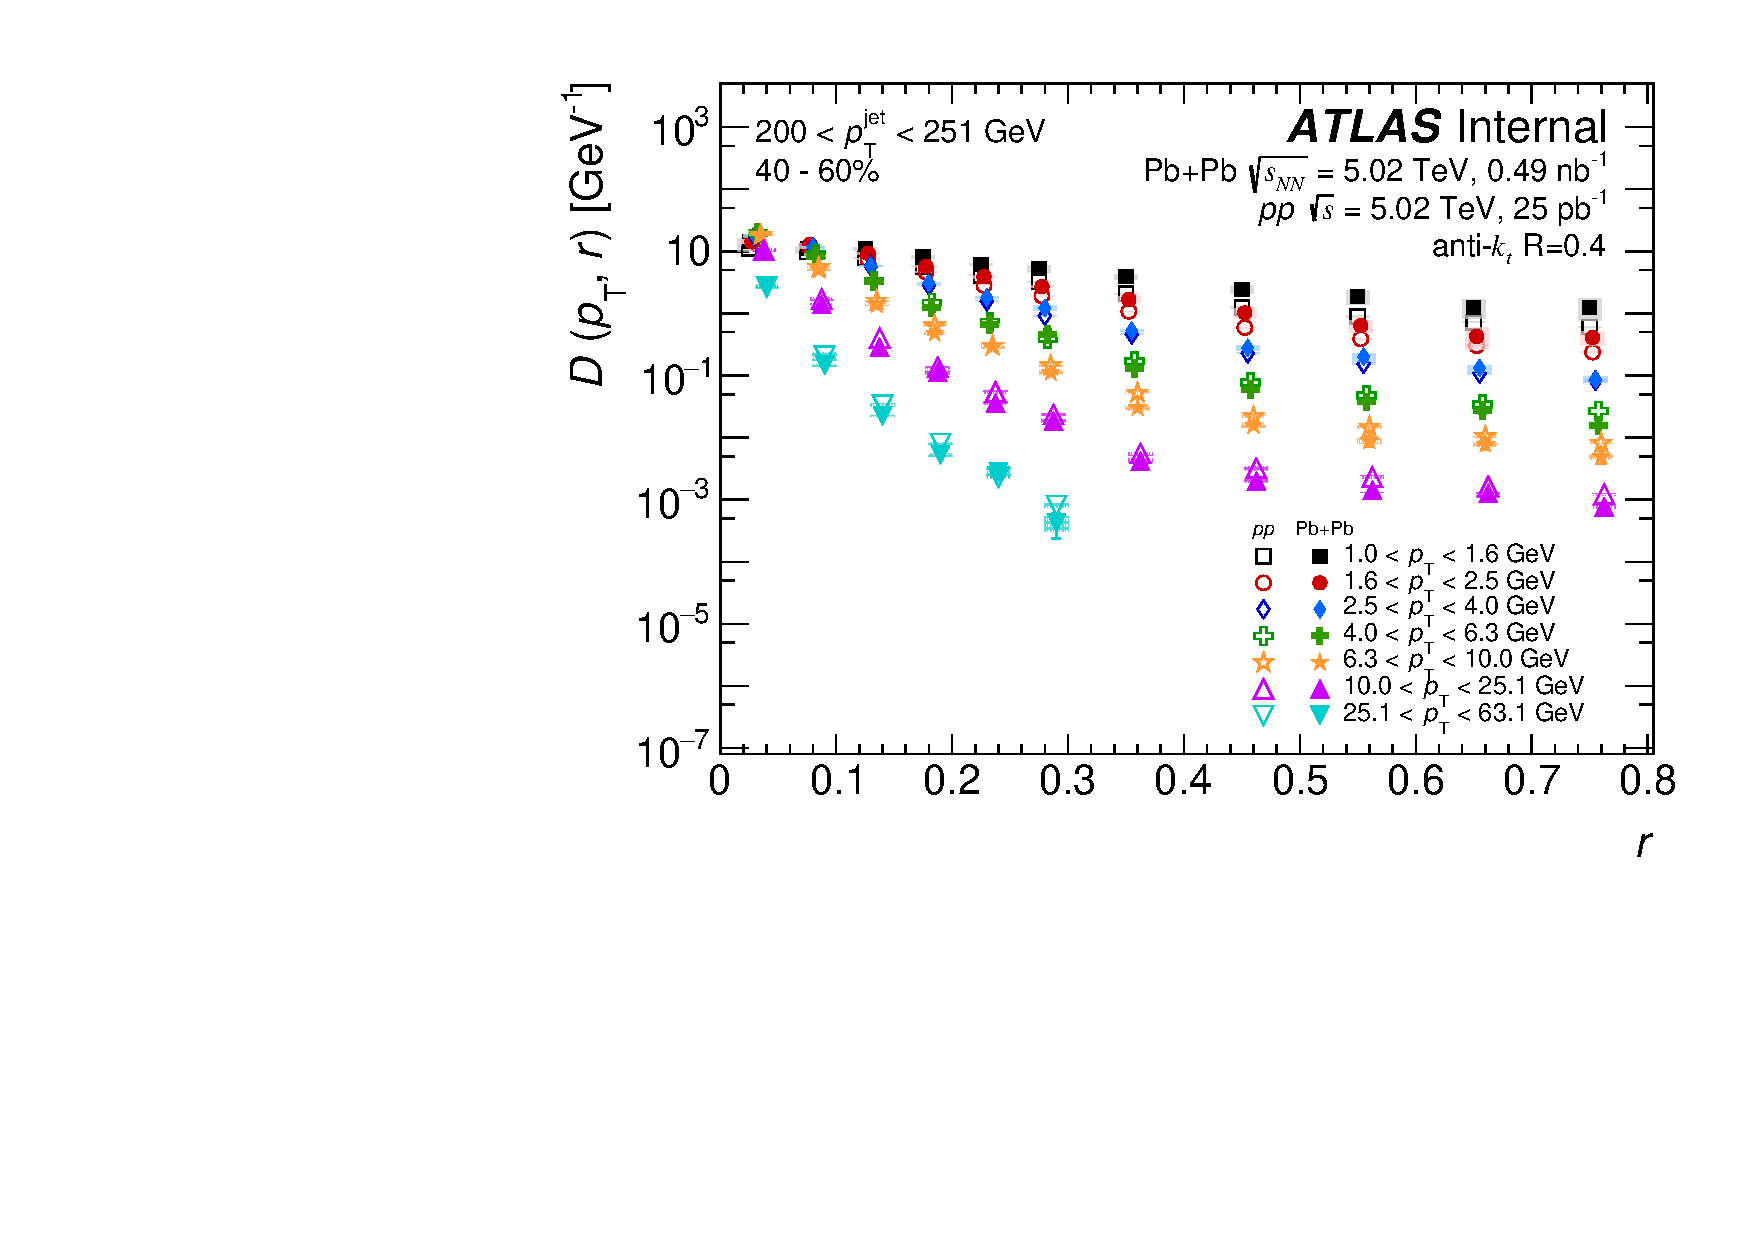
\includegraphics[width=0.48\textwidth]{figures/results/DpT_dR_jet9_cent4} &
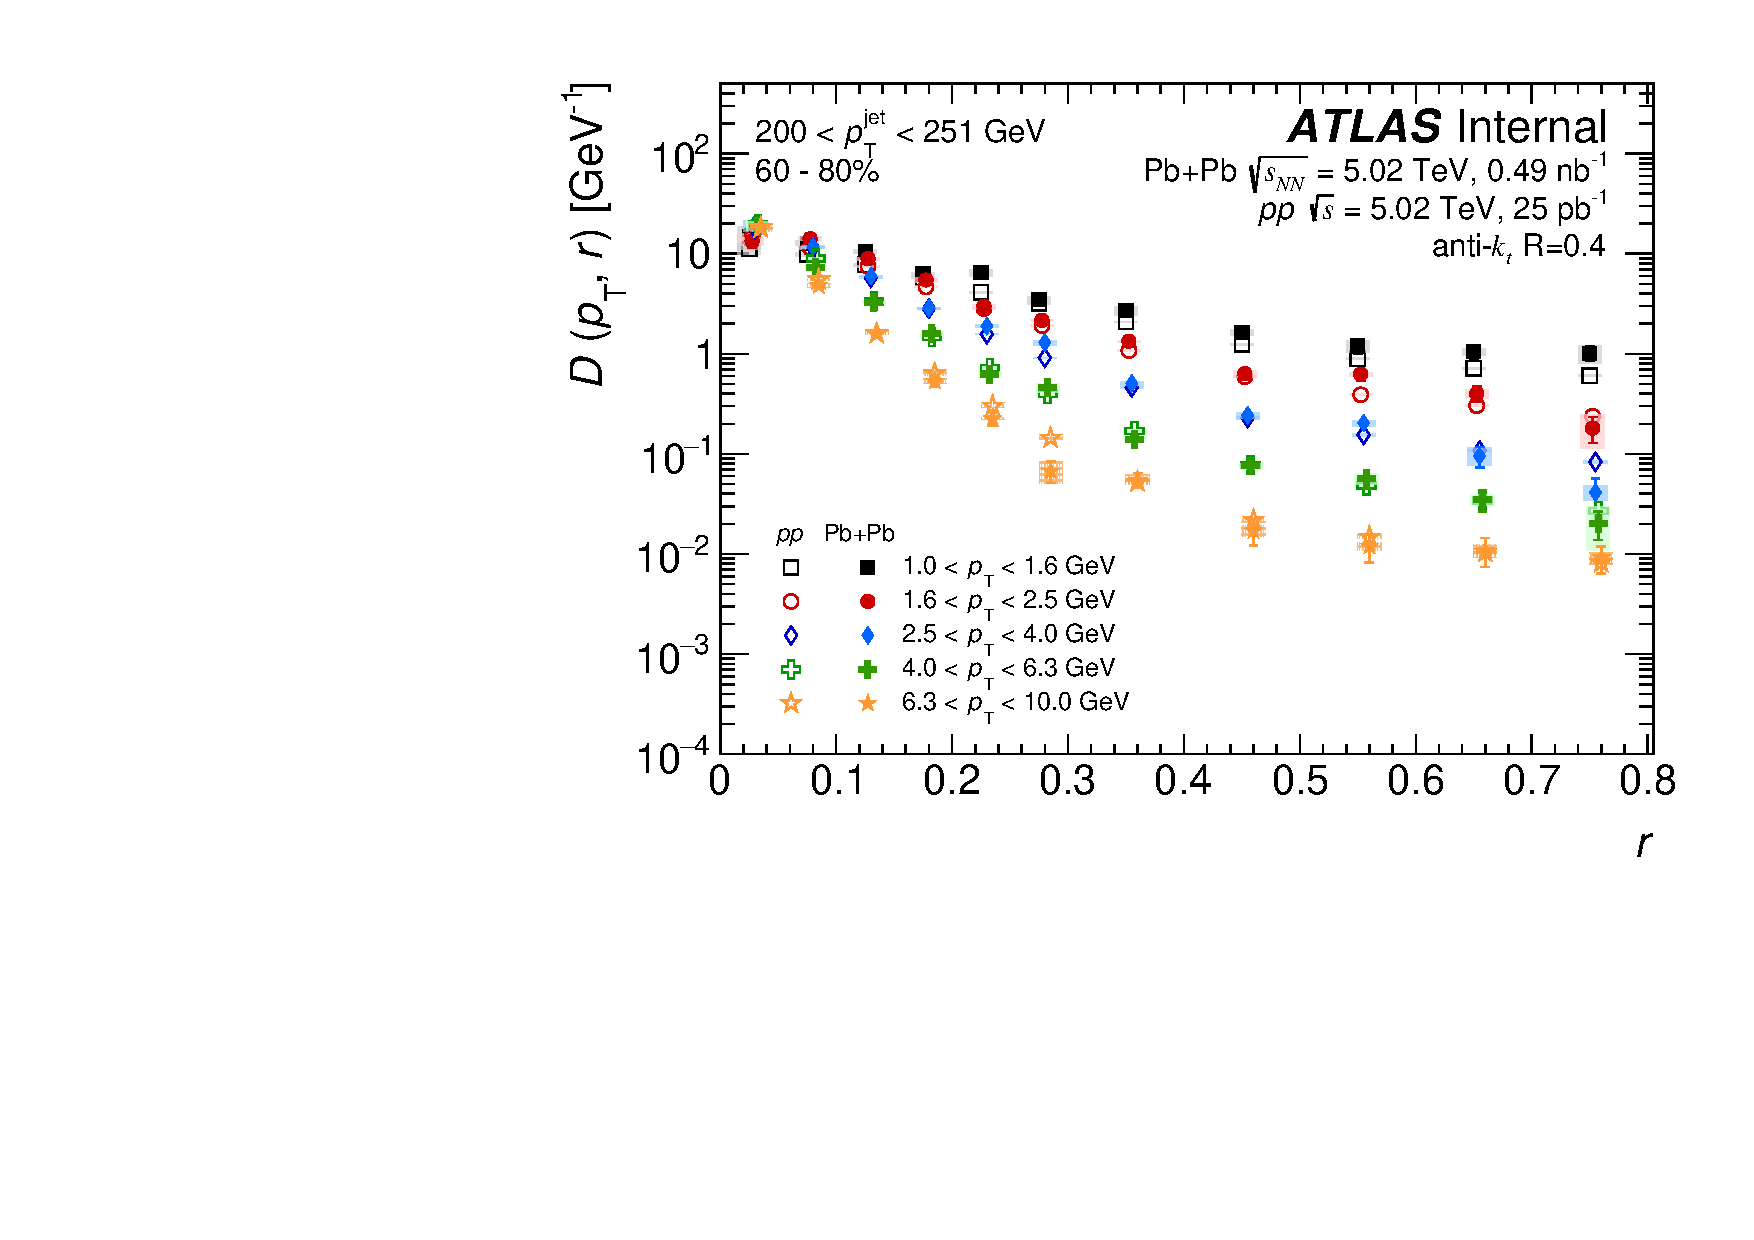
\includegraphics[width=0.48\textwidth]{figures/results/DpT_dR_jet9_cent5} \\
\end{tabular}}
\caption{ \Dptr\ distributions as a function of \rvar\ for different \pt\ ranges in 200--251 GeV jets.
The open markers are for \pp\ collisions and the solid markers are for \pbpb\ collisions.
The different panels refer to different centrality selections.
The vertical bars on the data points indicate statistical uncertainties while the shaded boxes indicate systematic uncertainties.
The widths of the boxes are not indicative of the bin size and the points are shifted horizontally for better visibility.
The distributions for $\pt > 6.3$ GeV are restricted to smaller \rvar\ values as discussed in Section~\ref{sec:analysis}.}
\label{fig:fullset_dptr_j9}
\end{figure}


\begin{figure}[h]
\centerline{
\begin{tabular}{ccc}
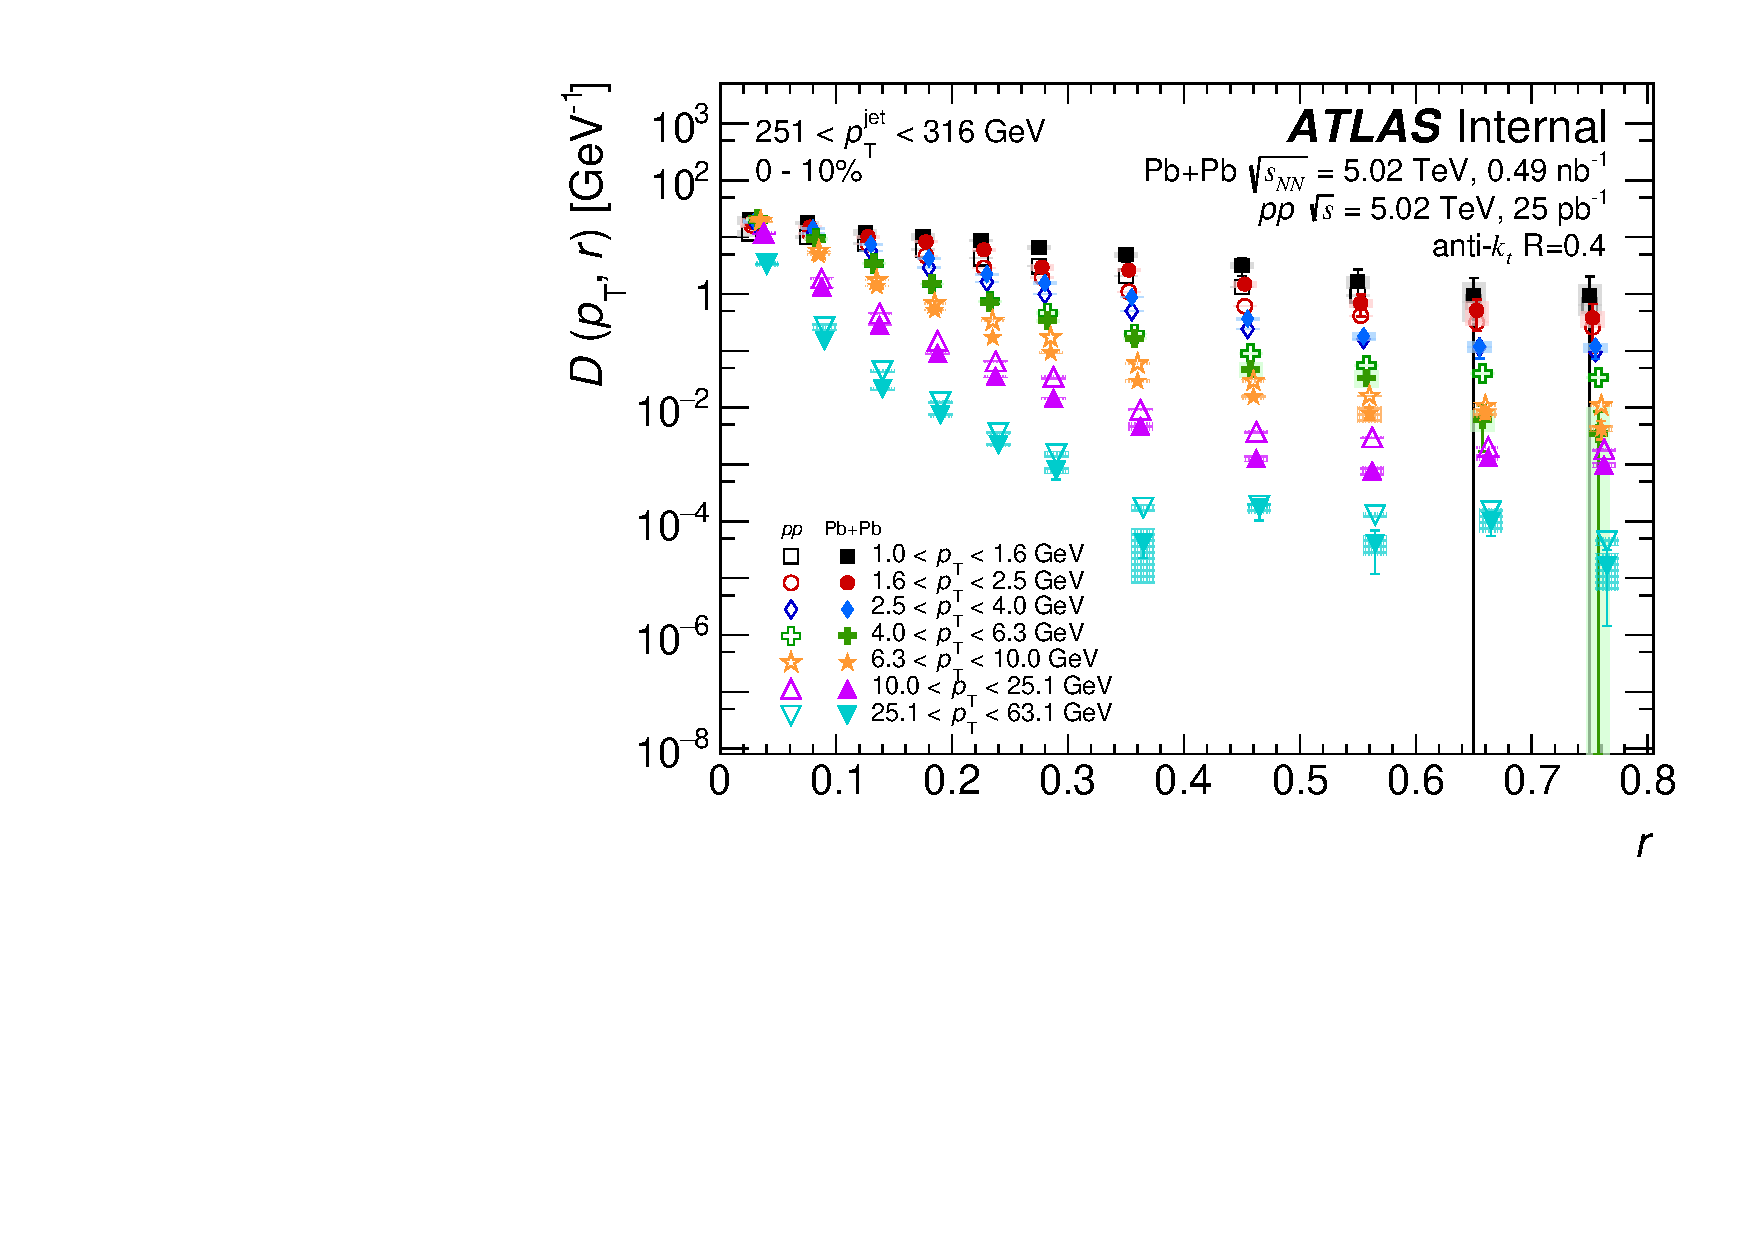
\includegraphics[width=0.48\textwidth]{figures/results/DpT_dR_jet10_cent0} &
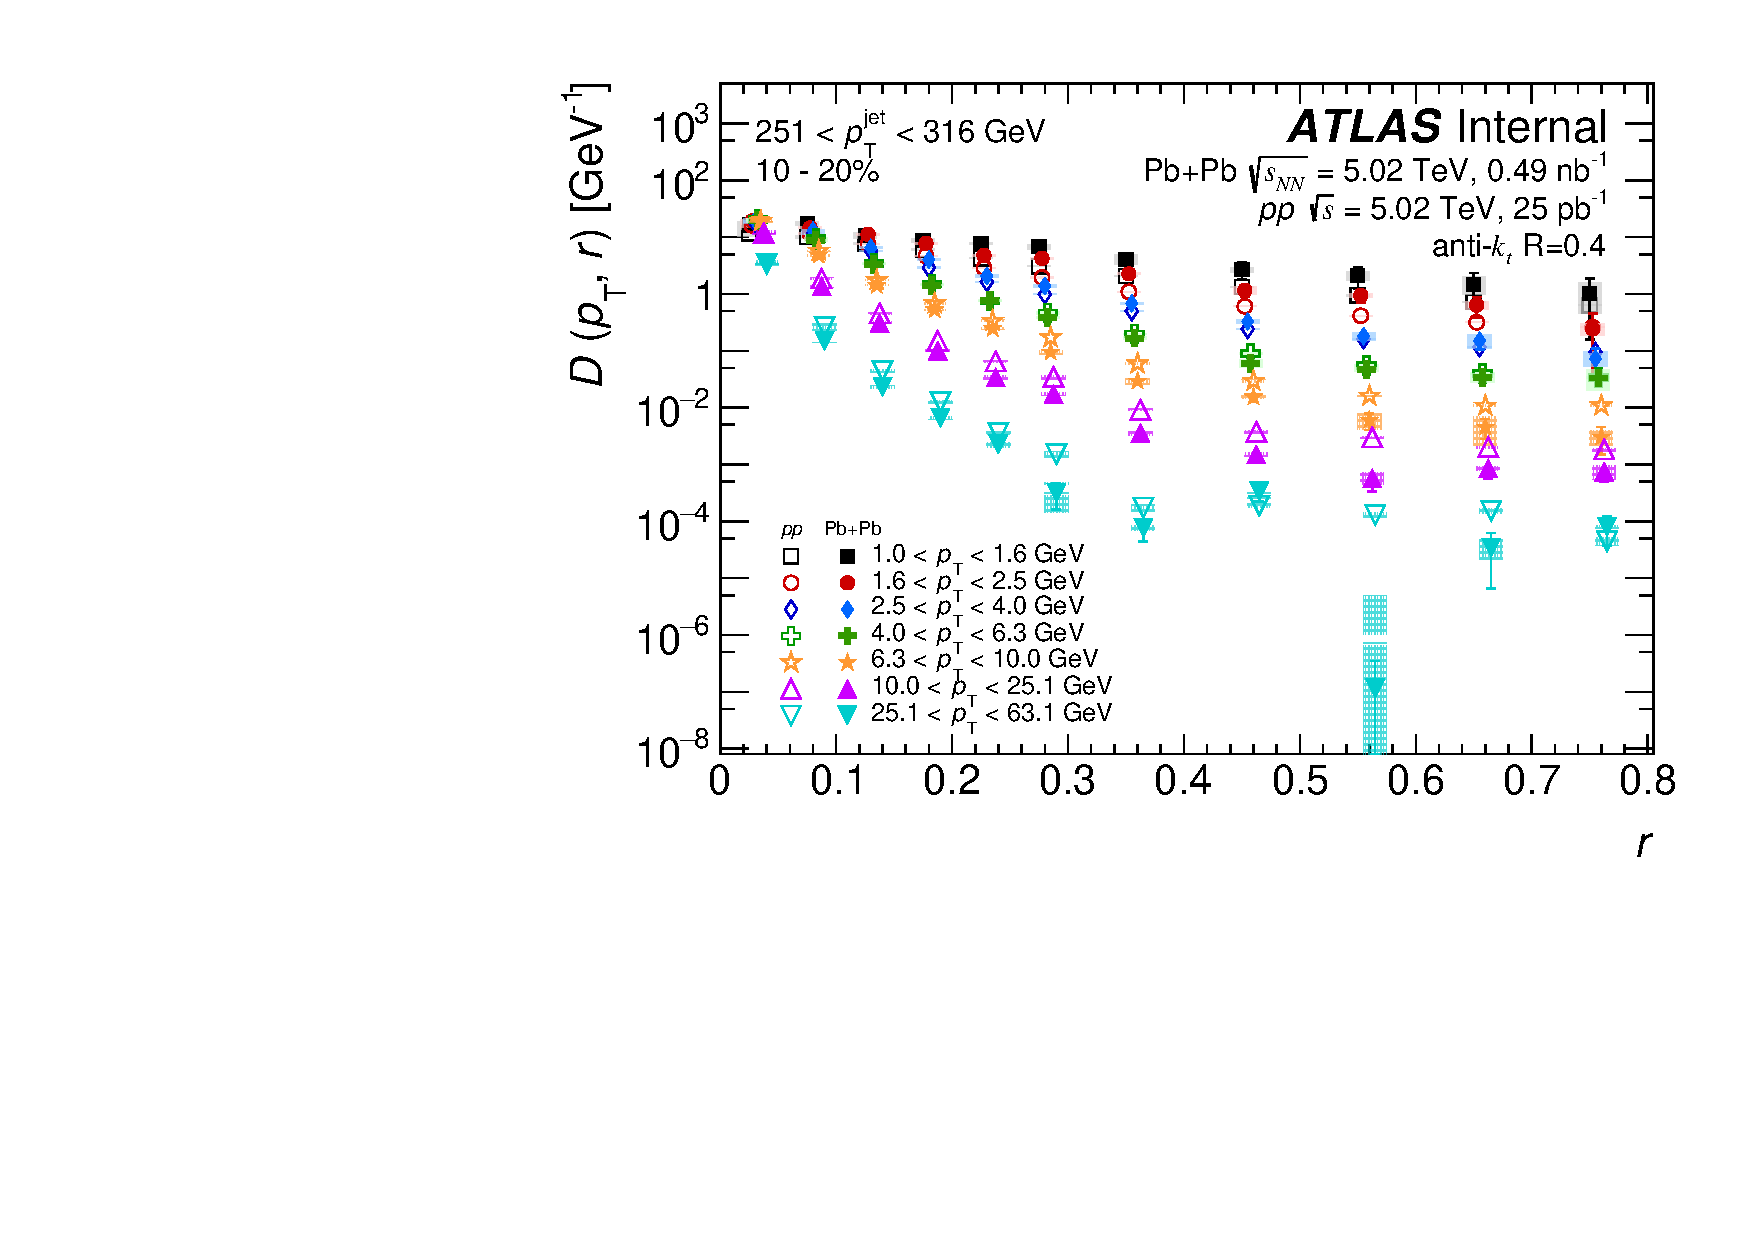
\includegraphics[width=0.48\textwidth]{figures/results/DpT_dR_jet10_cent1} \\
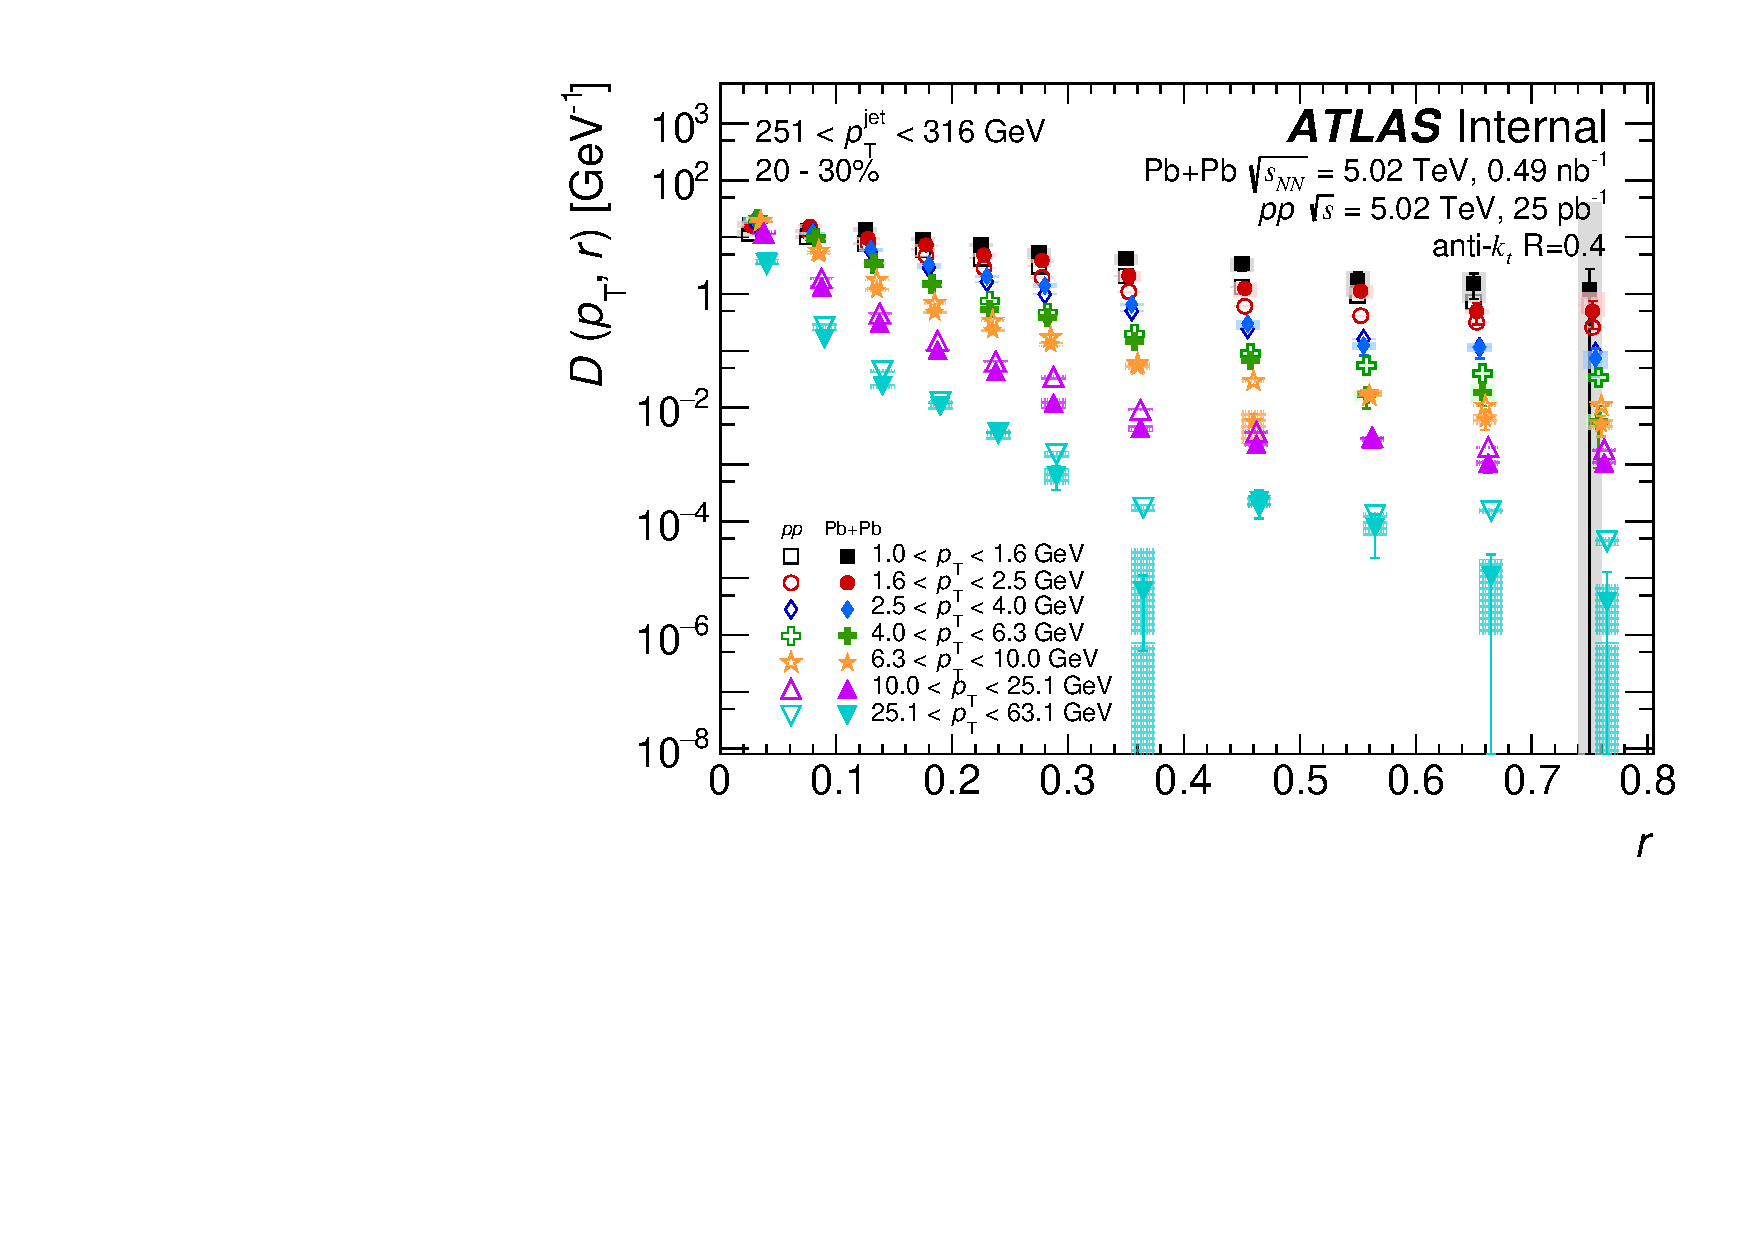
\includegraphics[width=0.48\textwidth]{figures/results/DpT_dR_jet10_cent2} &
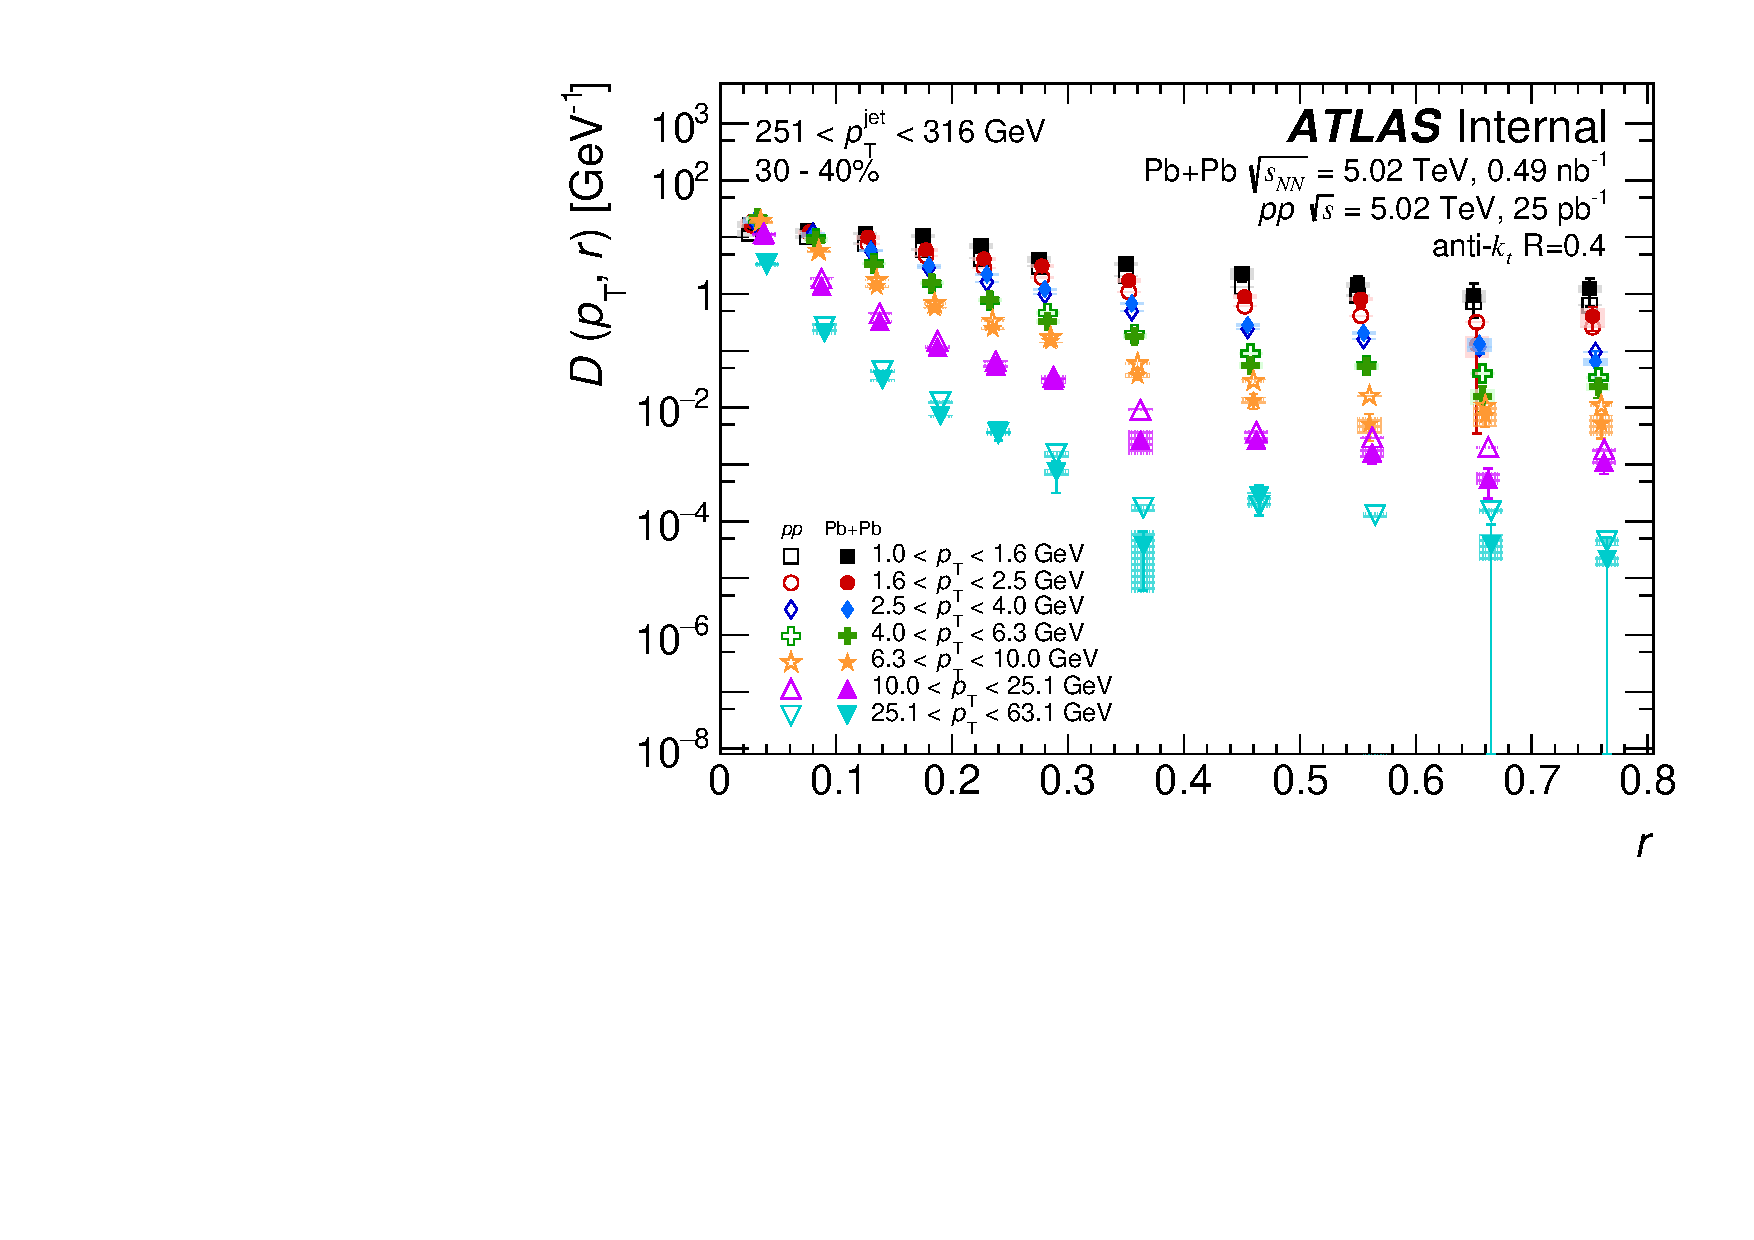
\includegraphics[width=0.48\textwidth]{figures/results/DpT_dR_jet10_cent3} \\
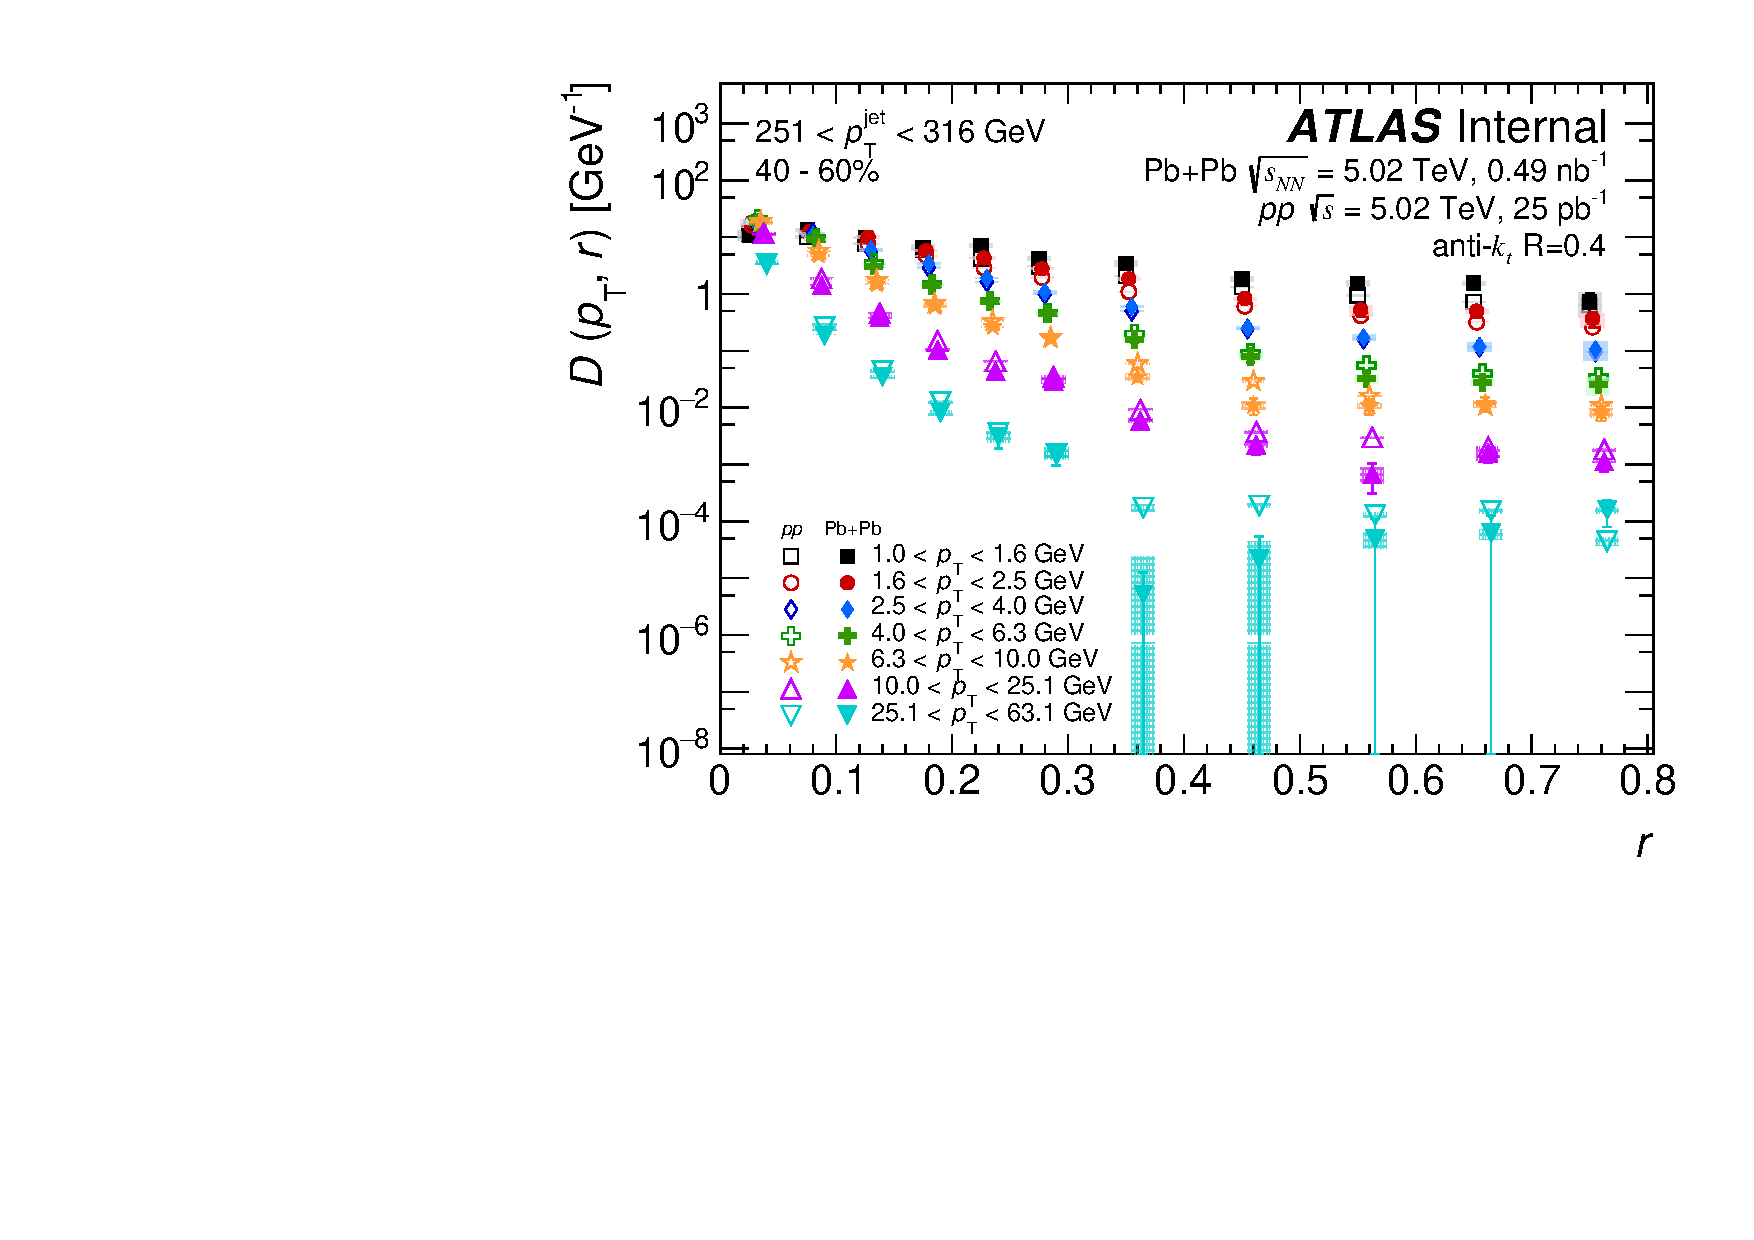
\includegraphics[width=0.48\textwidth]{figures/results/DpT_dR_jet10_cent4} &
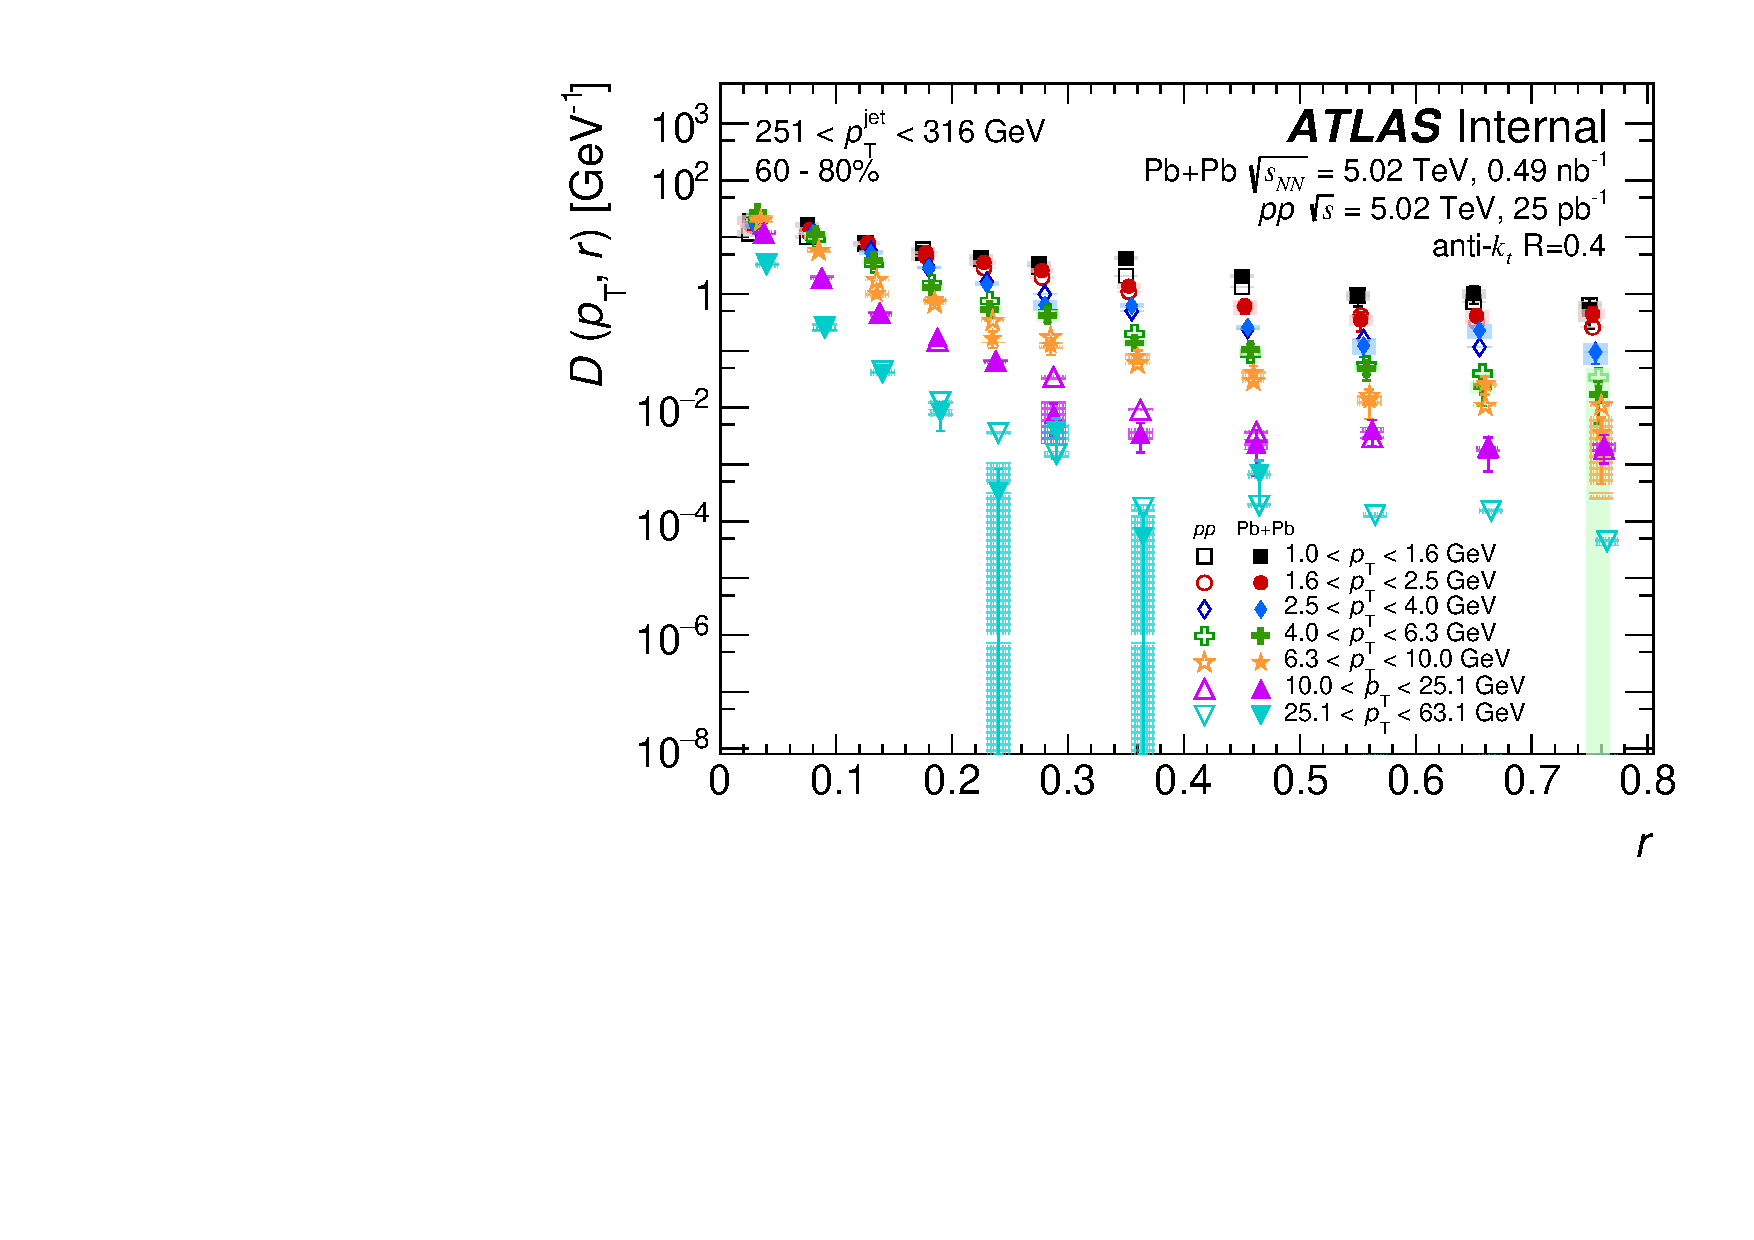
\includegraphics[width=0.48\textwidth]{figures/results/DpT_dR_jet10_cent5} \\
\end{tabular}}
\caption{ \Dptr\ distributions as a function of \rvar\ for different \pt\ ranges in 251--316 GeV jets.
The open markers are for \pp\ collisions and the solid markers are for \pbpb\ collisions.
The different panels refer to different centrality selections.
The vertical bars on the data points indicate statistical uncertainties while the shaded boxes indicate systematic uncertainties.
The widths of the boxes are not indicative of the bin size and the points are shifted horizontally for better visibility.}
\label{fig:fullset_dptr_j10}
\end{figure}




\begin{figure}[h]
\centerline{
\begin{tabular}{ccc}
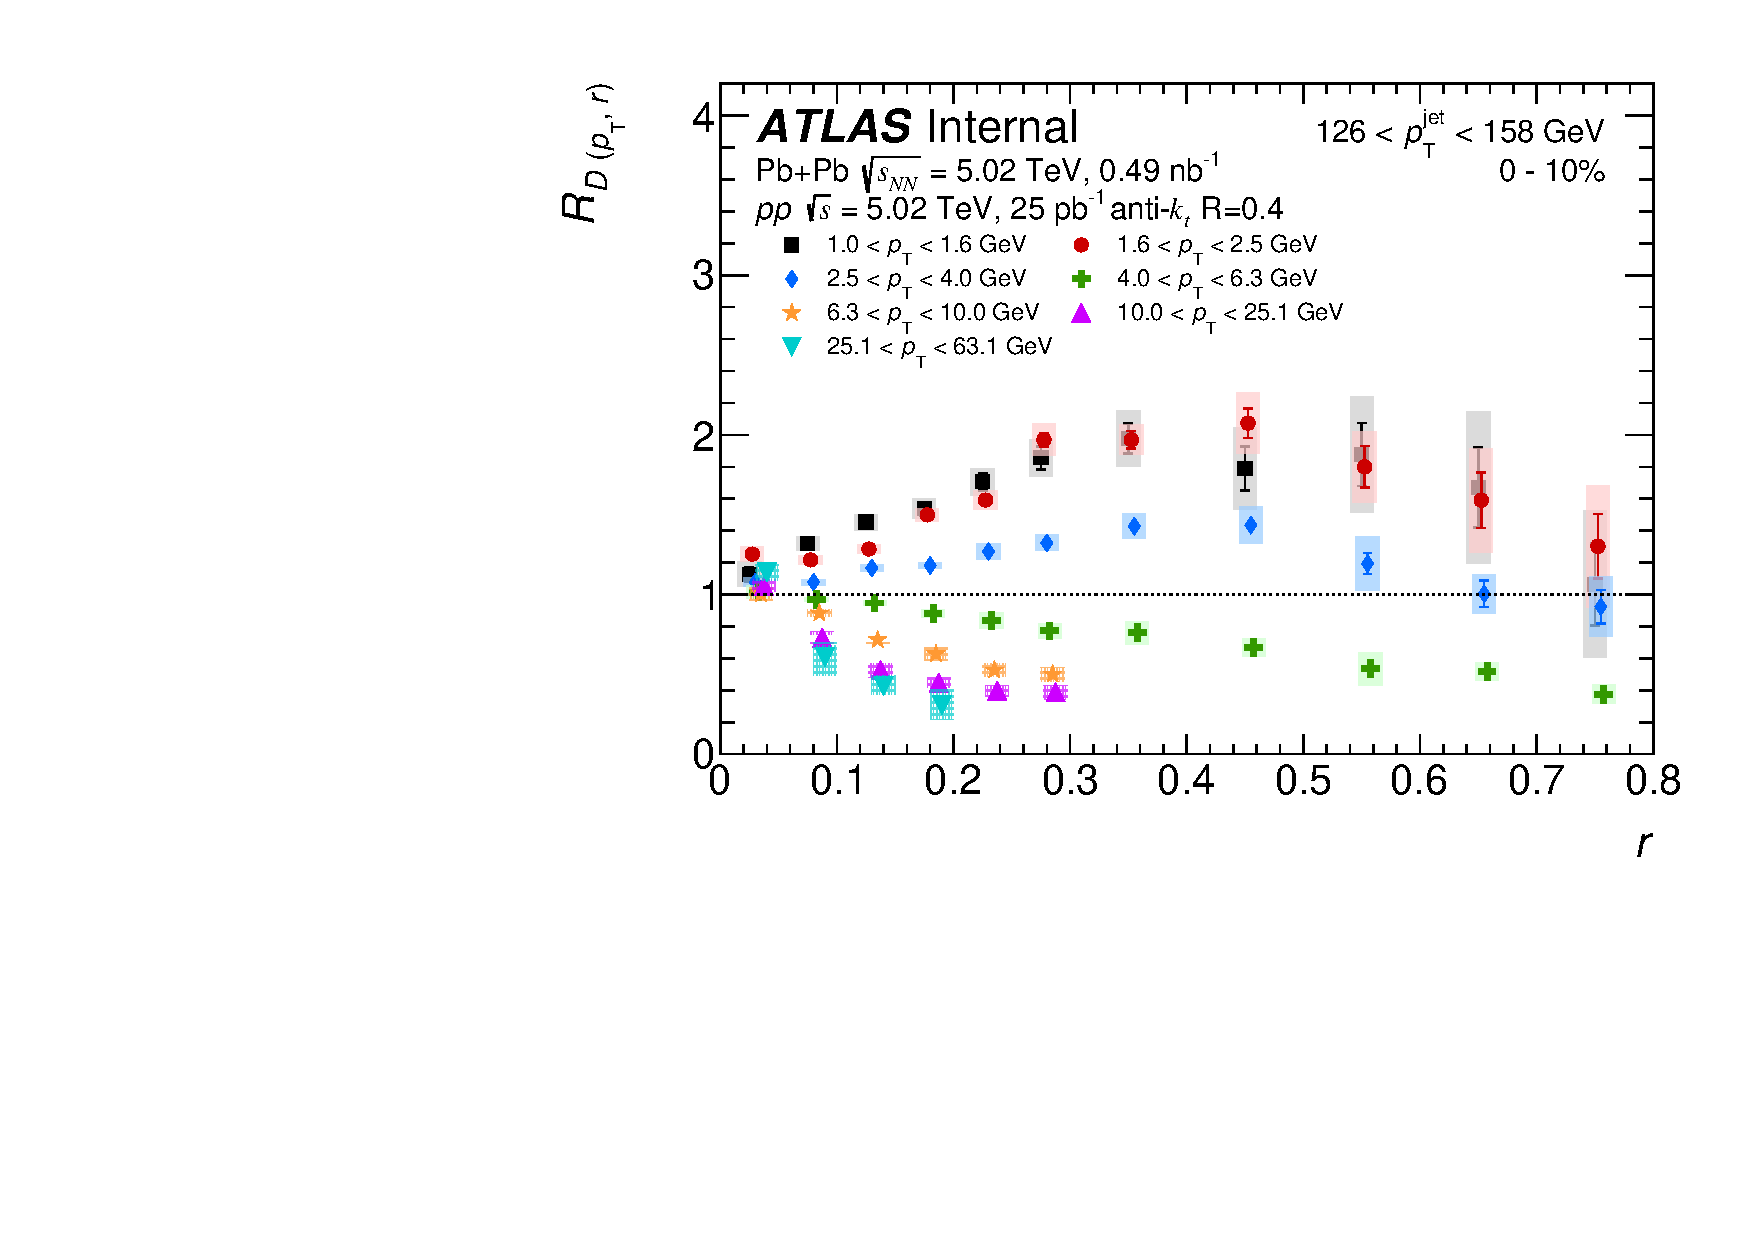
\includegraphics[width=0.48\textwidth]{figures/results/RDpT_dR_jet7_cent0} &
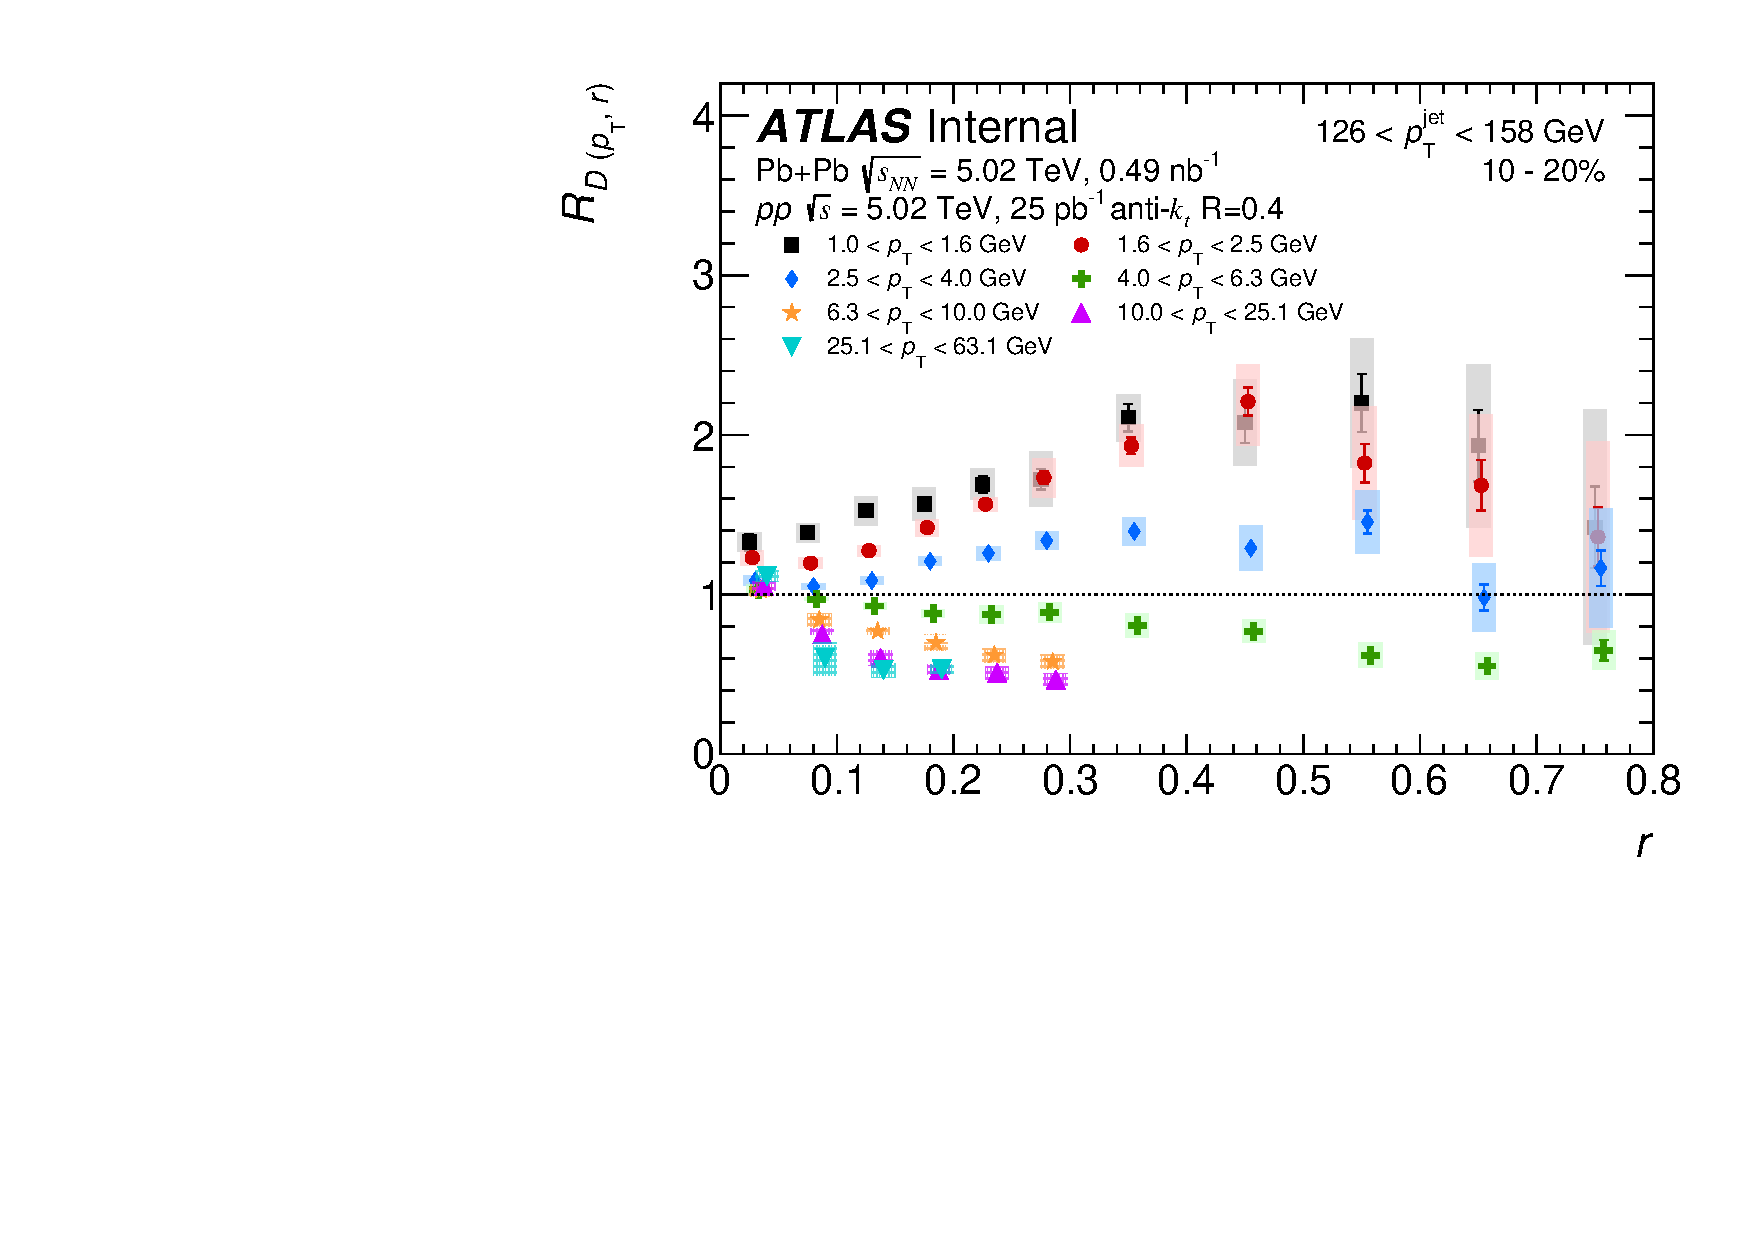
\includegraphics[width=0.48\textwidth]{figures/results/RDpT_dR_jet7_cent1} \\
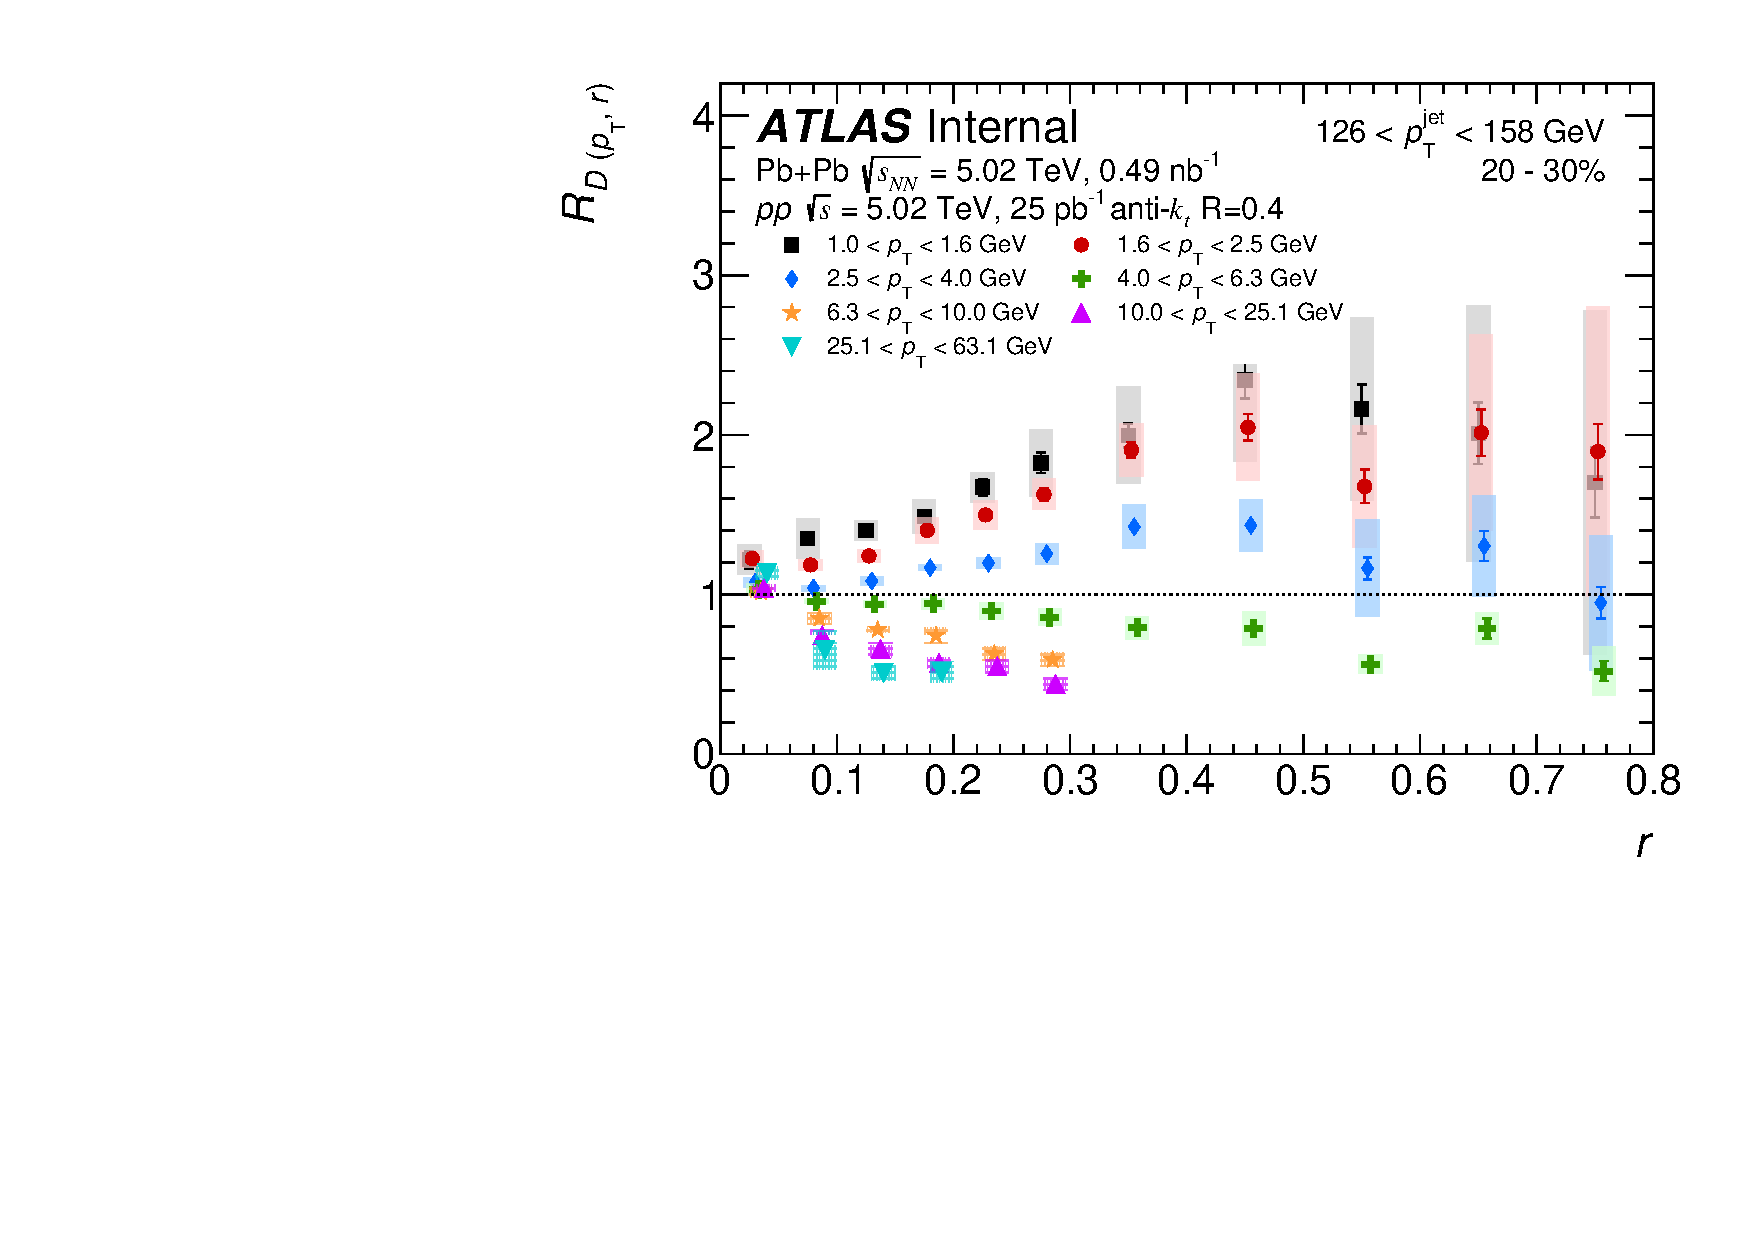
\includegraphics[width=0.48\textwidth]{figures/results/RDpT_dR_jet7_cent2} &
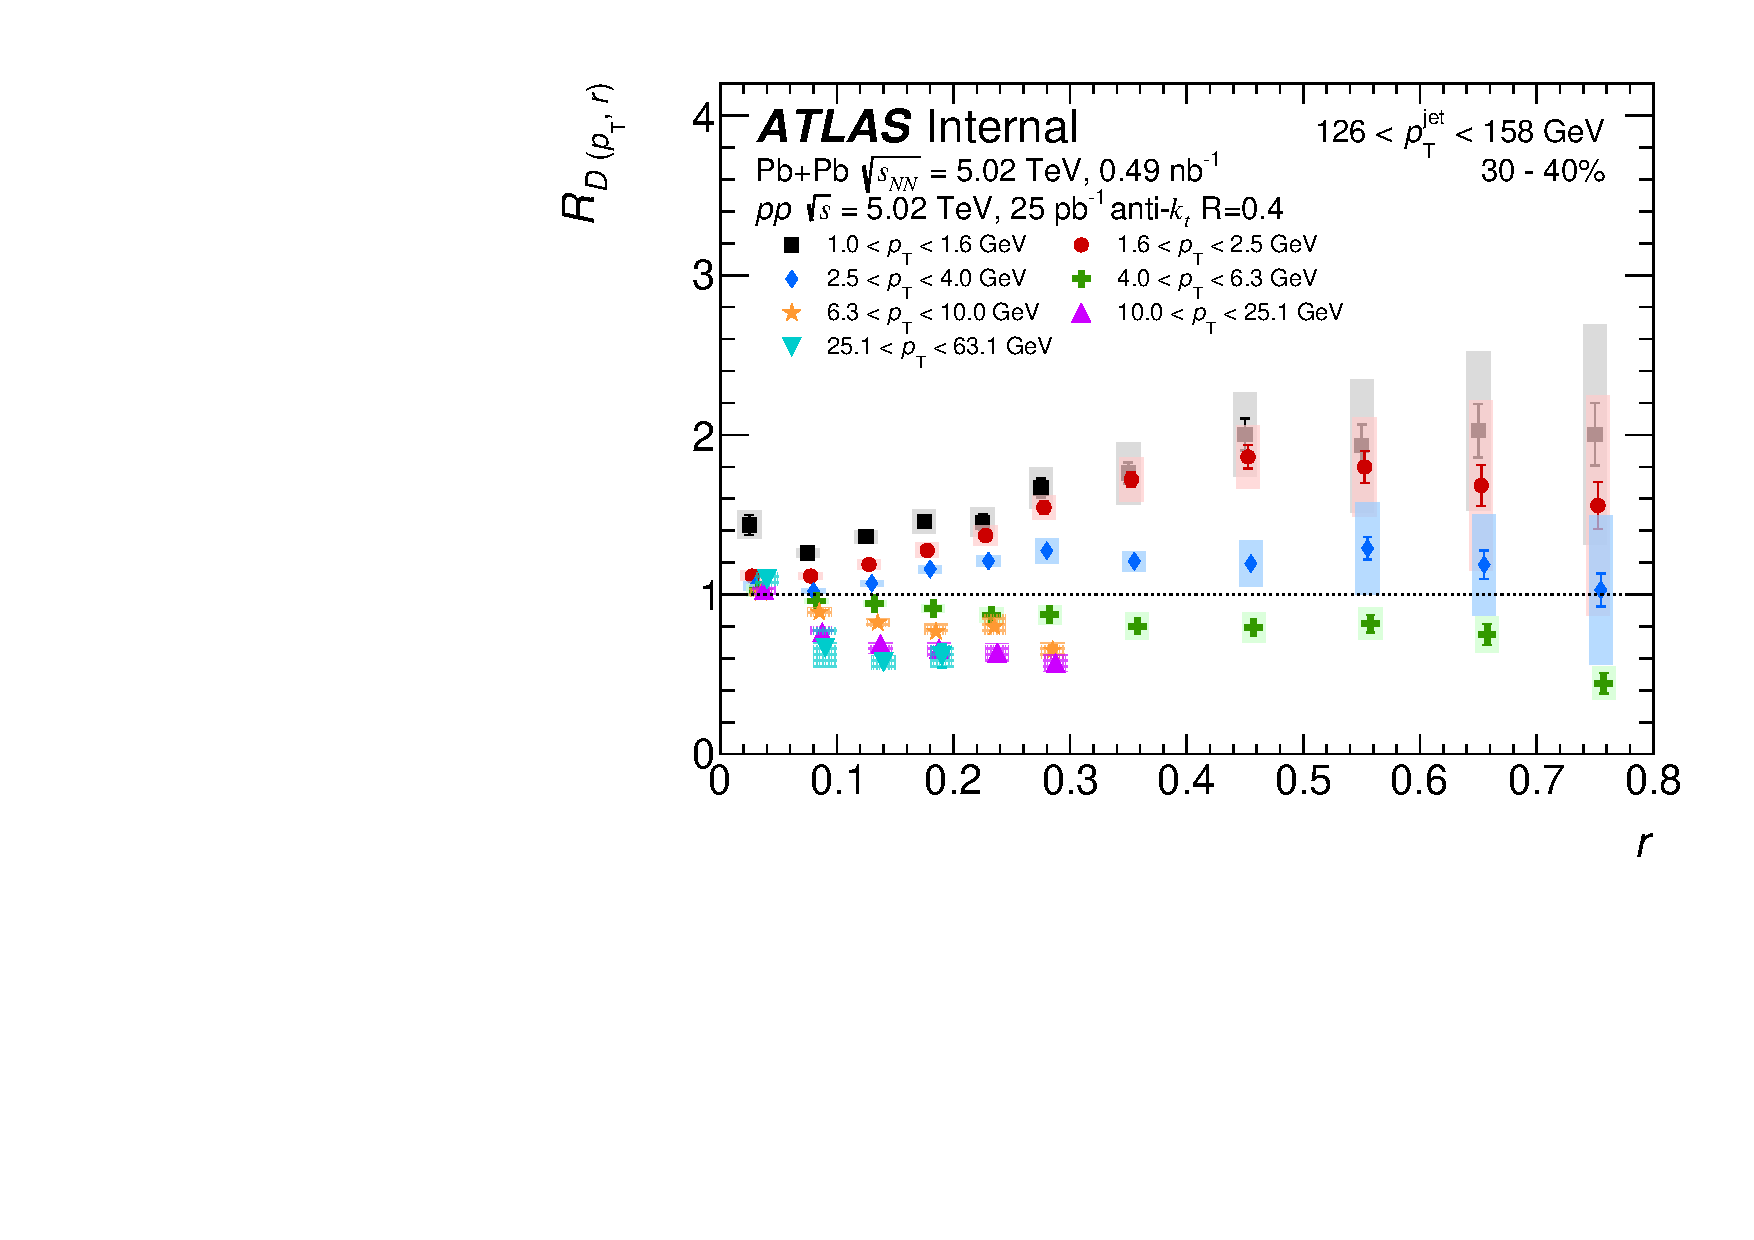
\includegraphics[width=0.48\textwidth]{figures/results/RDpT_dR_jet7_cent3} \\
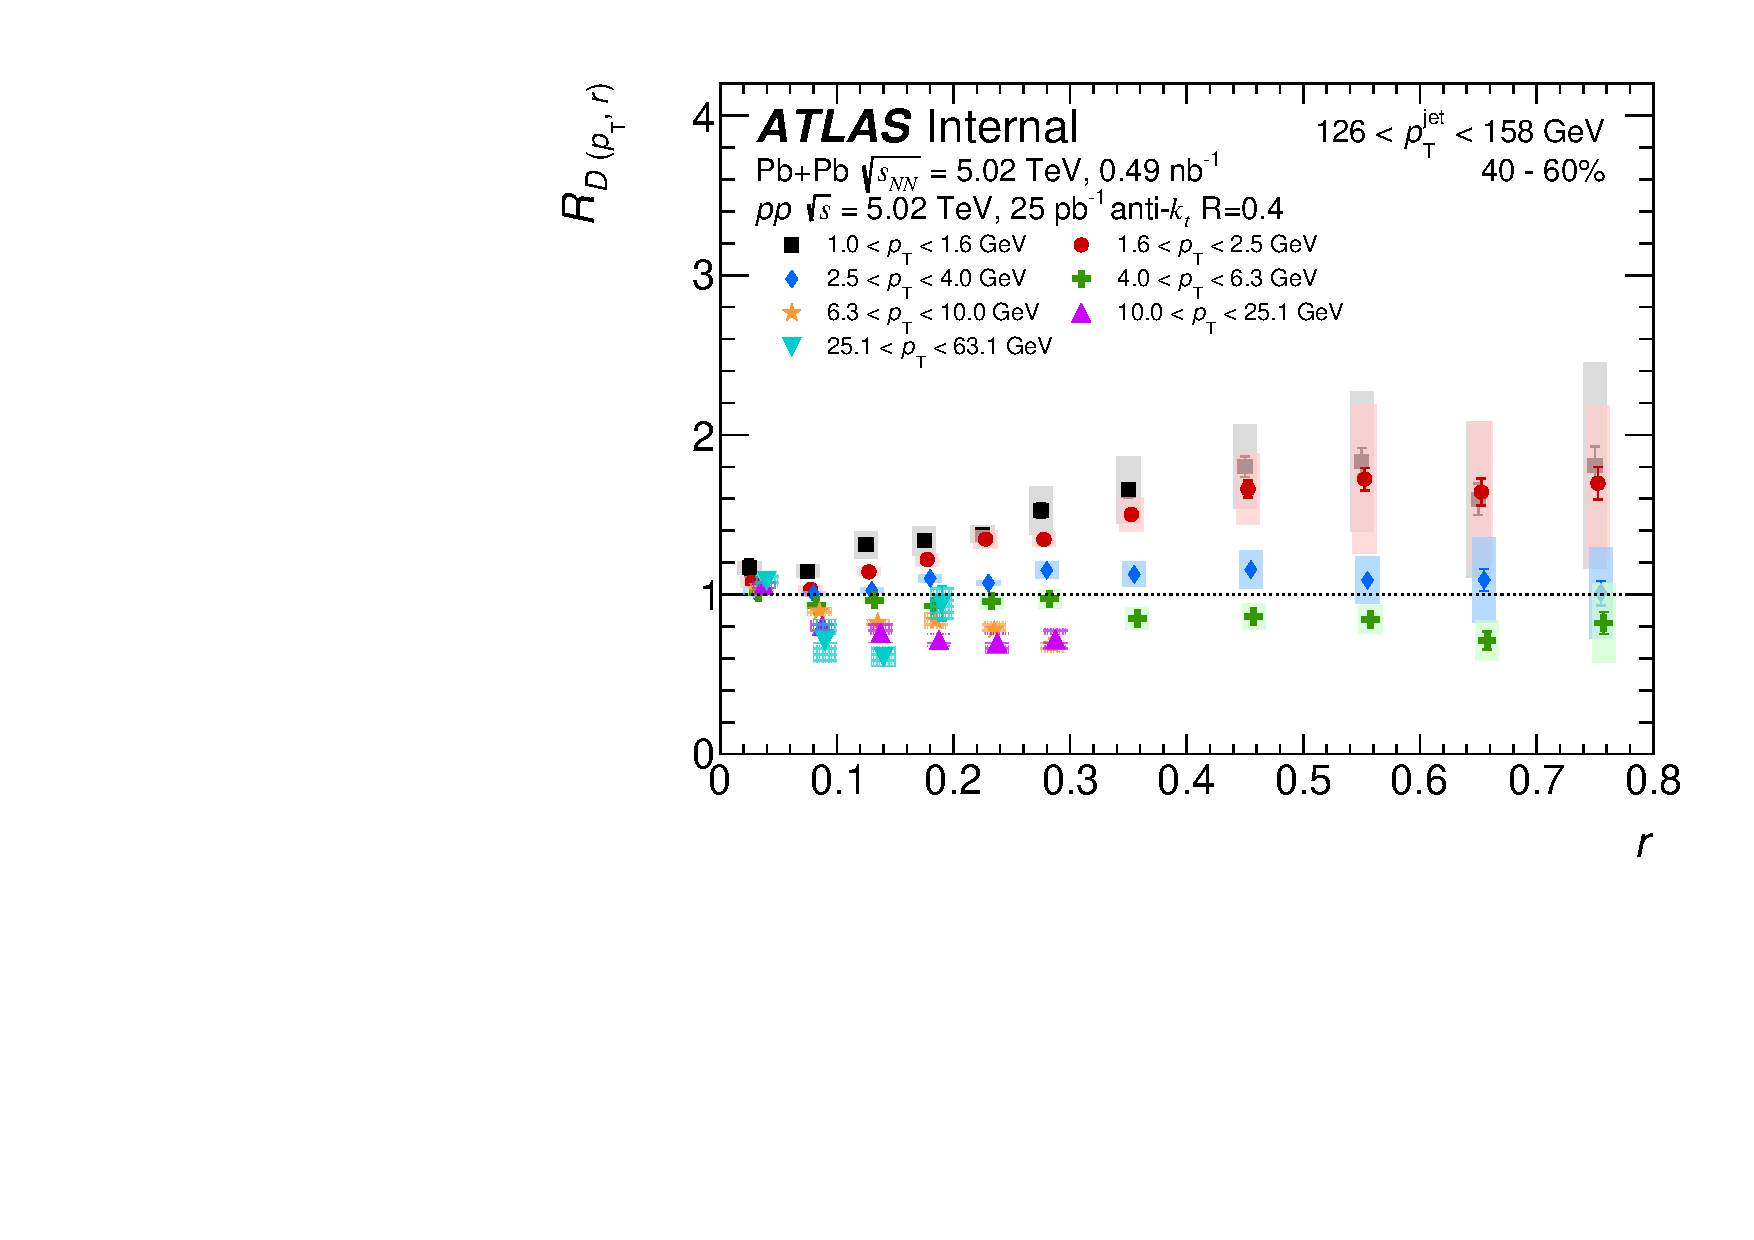
\includegraphics[width=0.48\textwidth]{figures/results/RDpT_dR_jet7_cent4} &
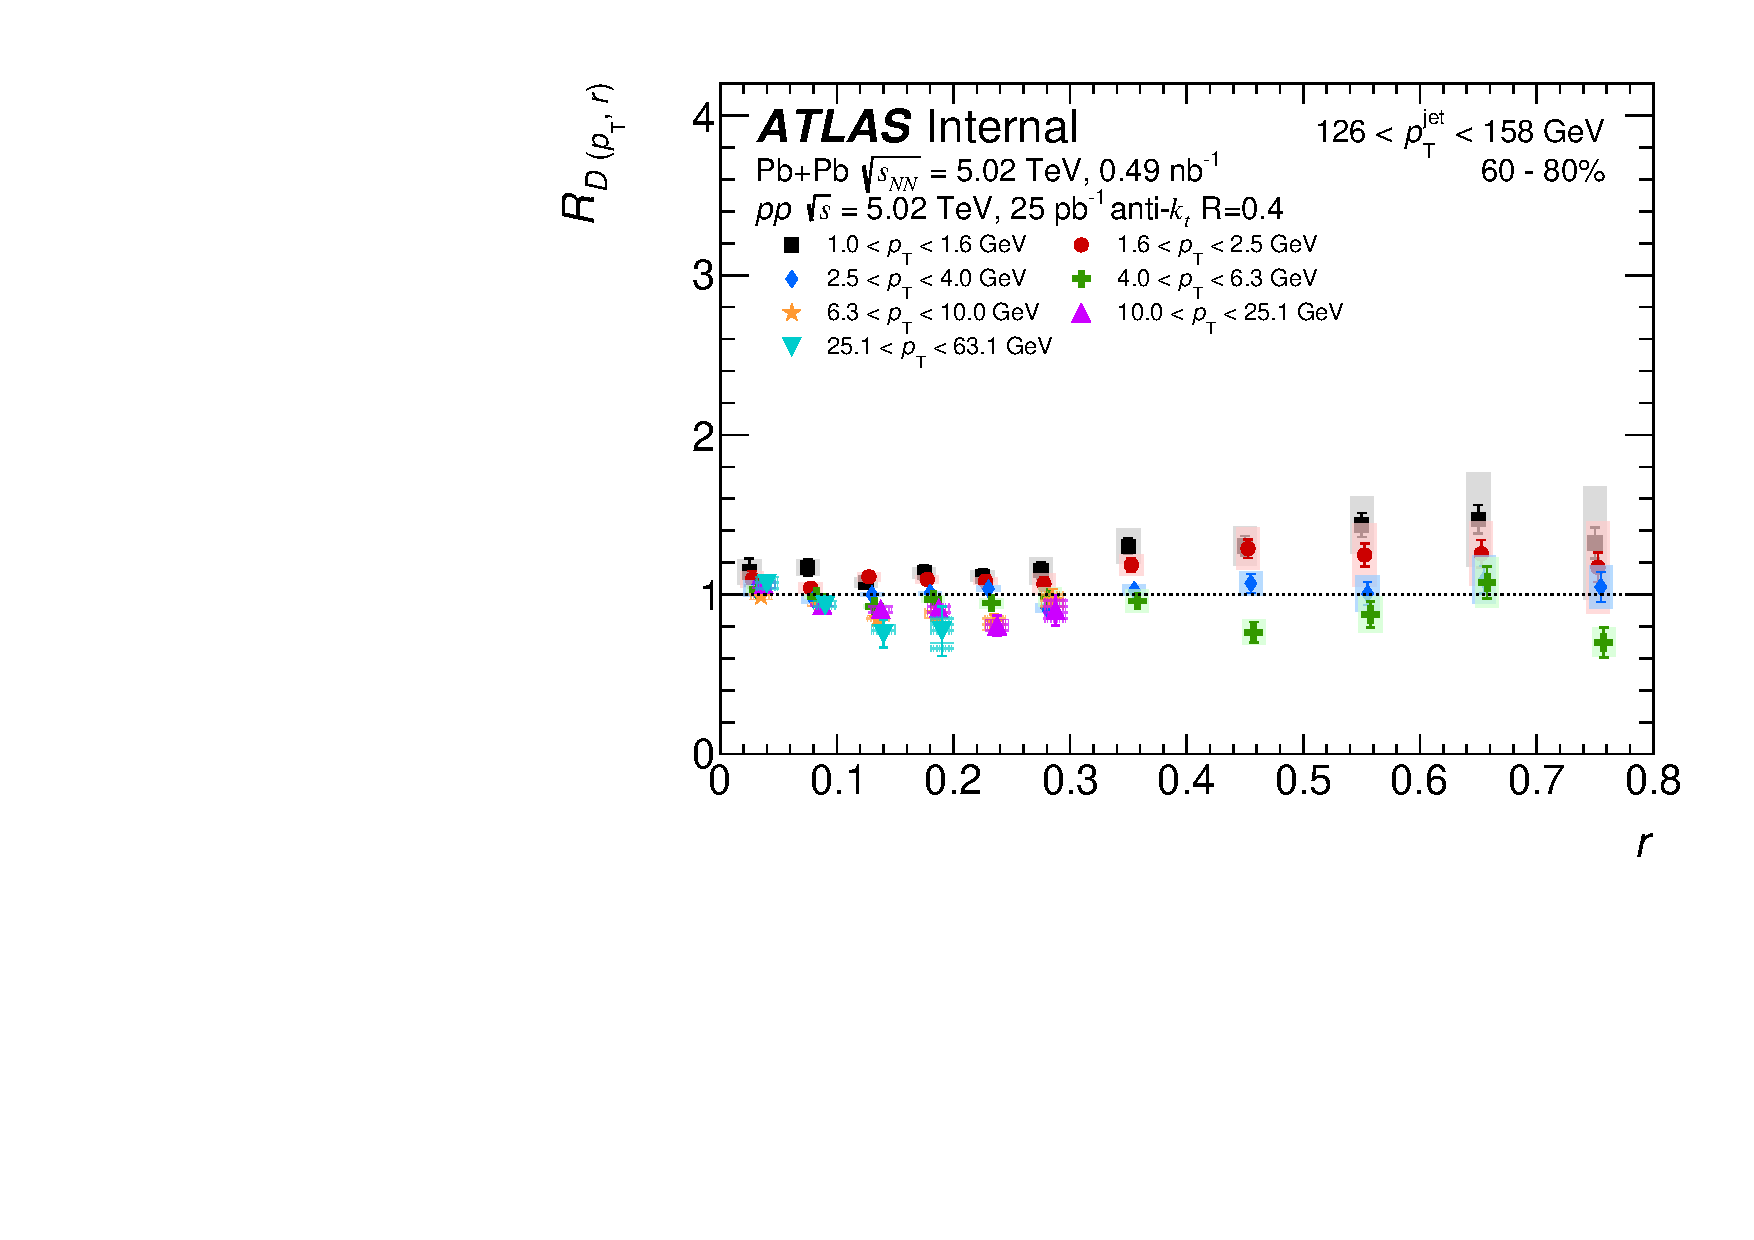
\includegraphics[width=0.48\textwidth]{figures/results/RDpT_dR_jet7_cent5} \\
\end{tabular}}
\caption{ The \RDptr\ distributions as a function of \rvar\ for different \pt\ selections in 126--158 GeV jets.
The different panels refer to different centrality selections.
The vertical bars on the data points indicate statistical uncertainties while the shaded boxes indicate systematic uncertainties.
The widths of the boxes are not indicative of the bin size and the points are shifted horizontally for better visibility.}
\label{fig:fullset_rptr_j7}
\end{figure}

\begin{figure}[h]
\centerline{
\begin{tabular}{ccc}
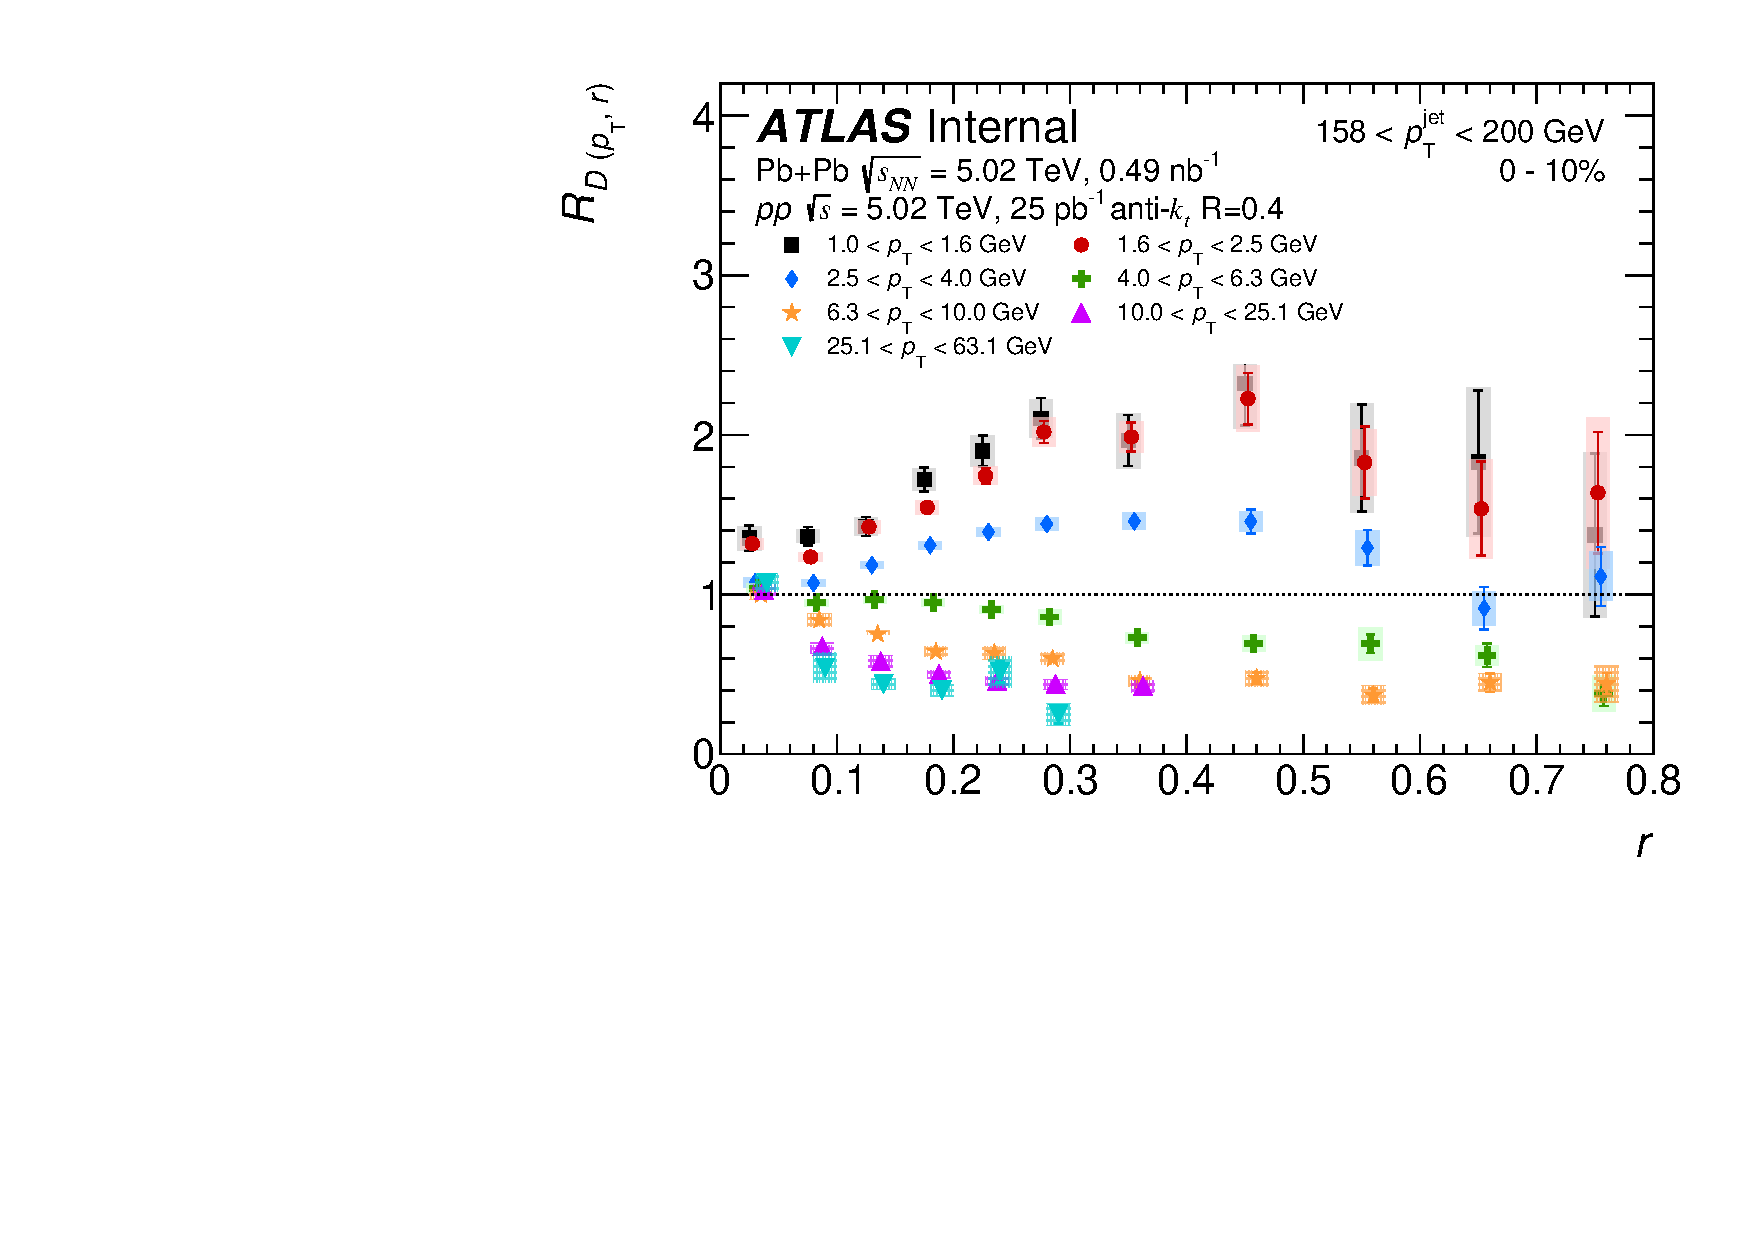
\includegraphics[width=0.48\textwidth]{figures/results/RDpT_dR_jet8_cent0} &
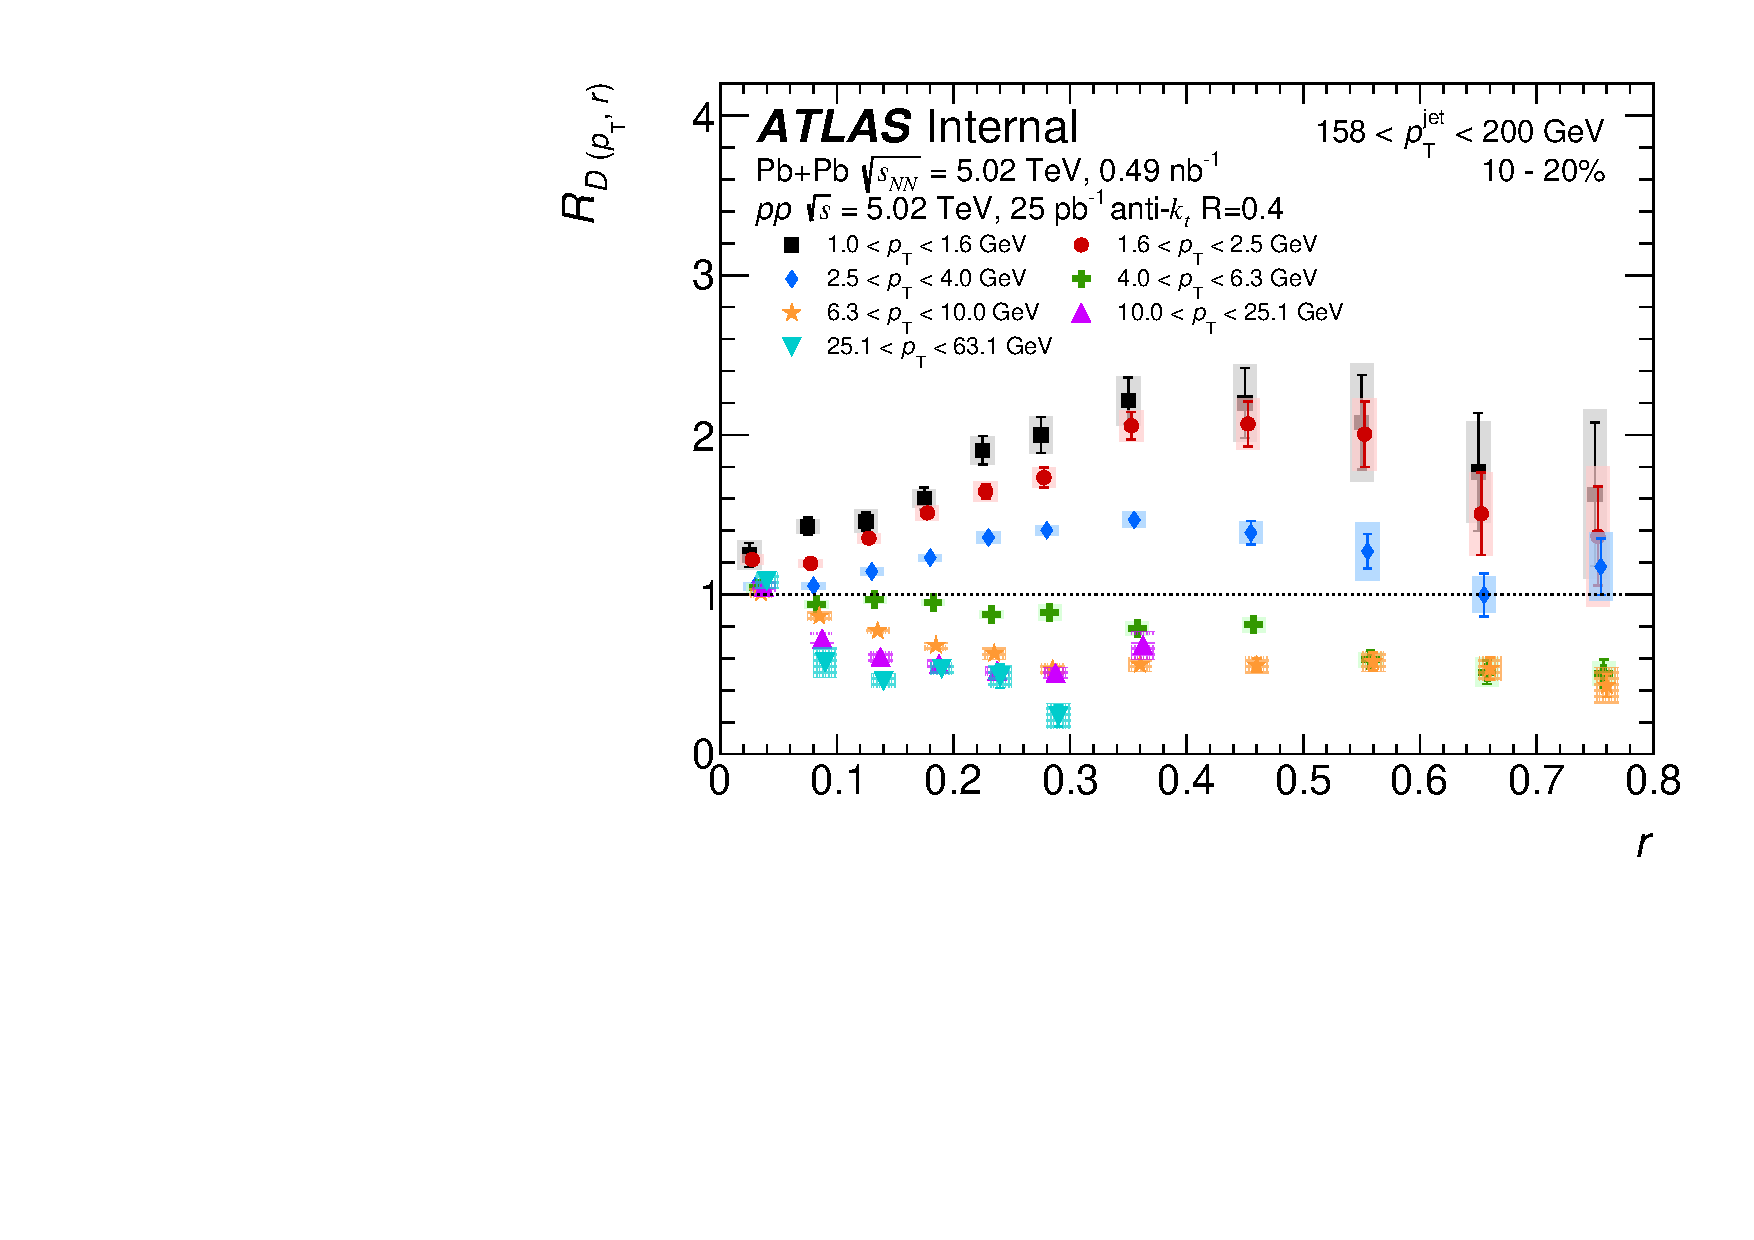
\includegraphics[width=0.48\textwidth]{figures/results/RDpT_dR_jet8_cent1} \\
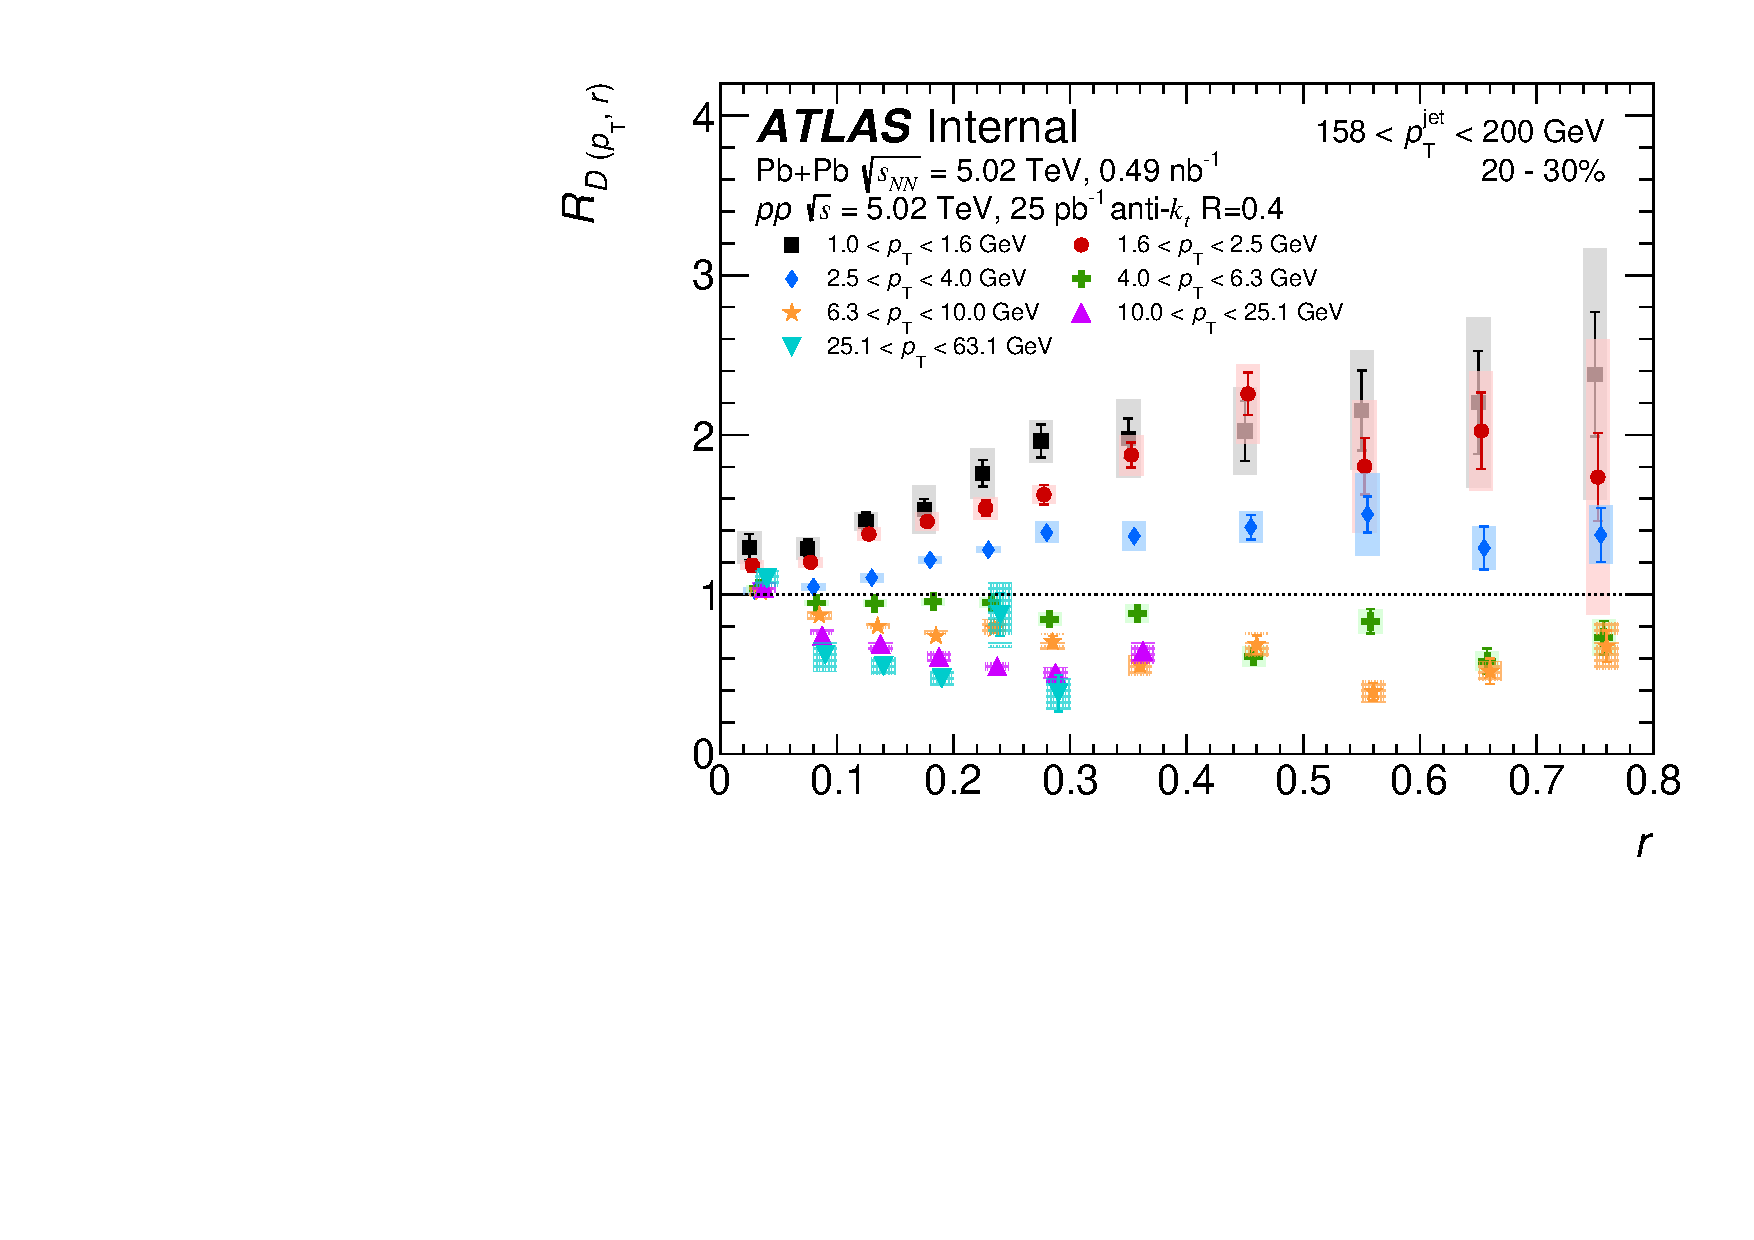
\includegraphics[width=0.48\textwidth]{figures/results/RDpT_dR_jet8_cent2} &
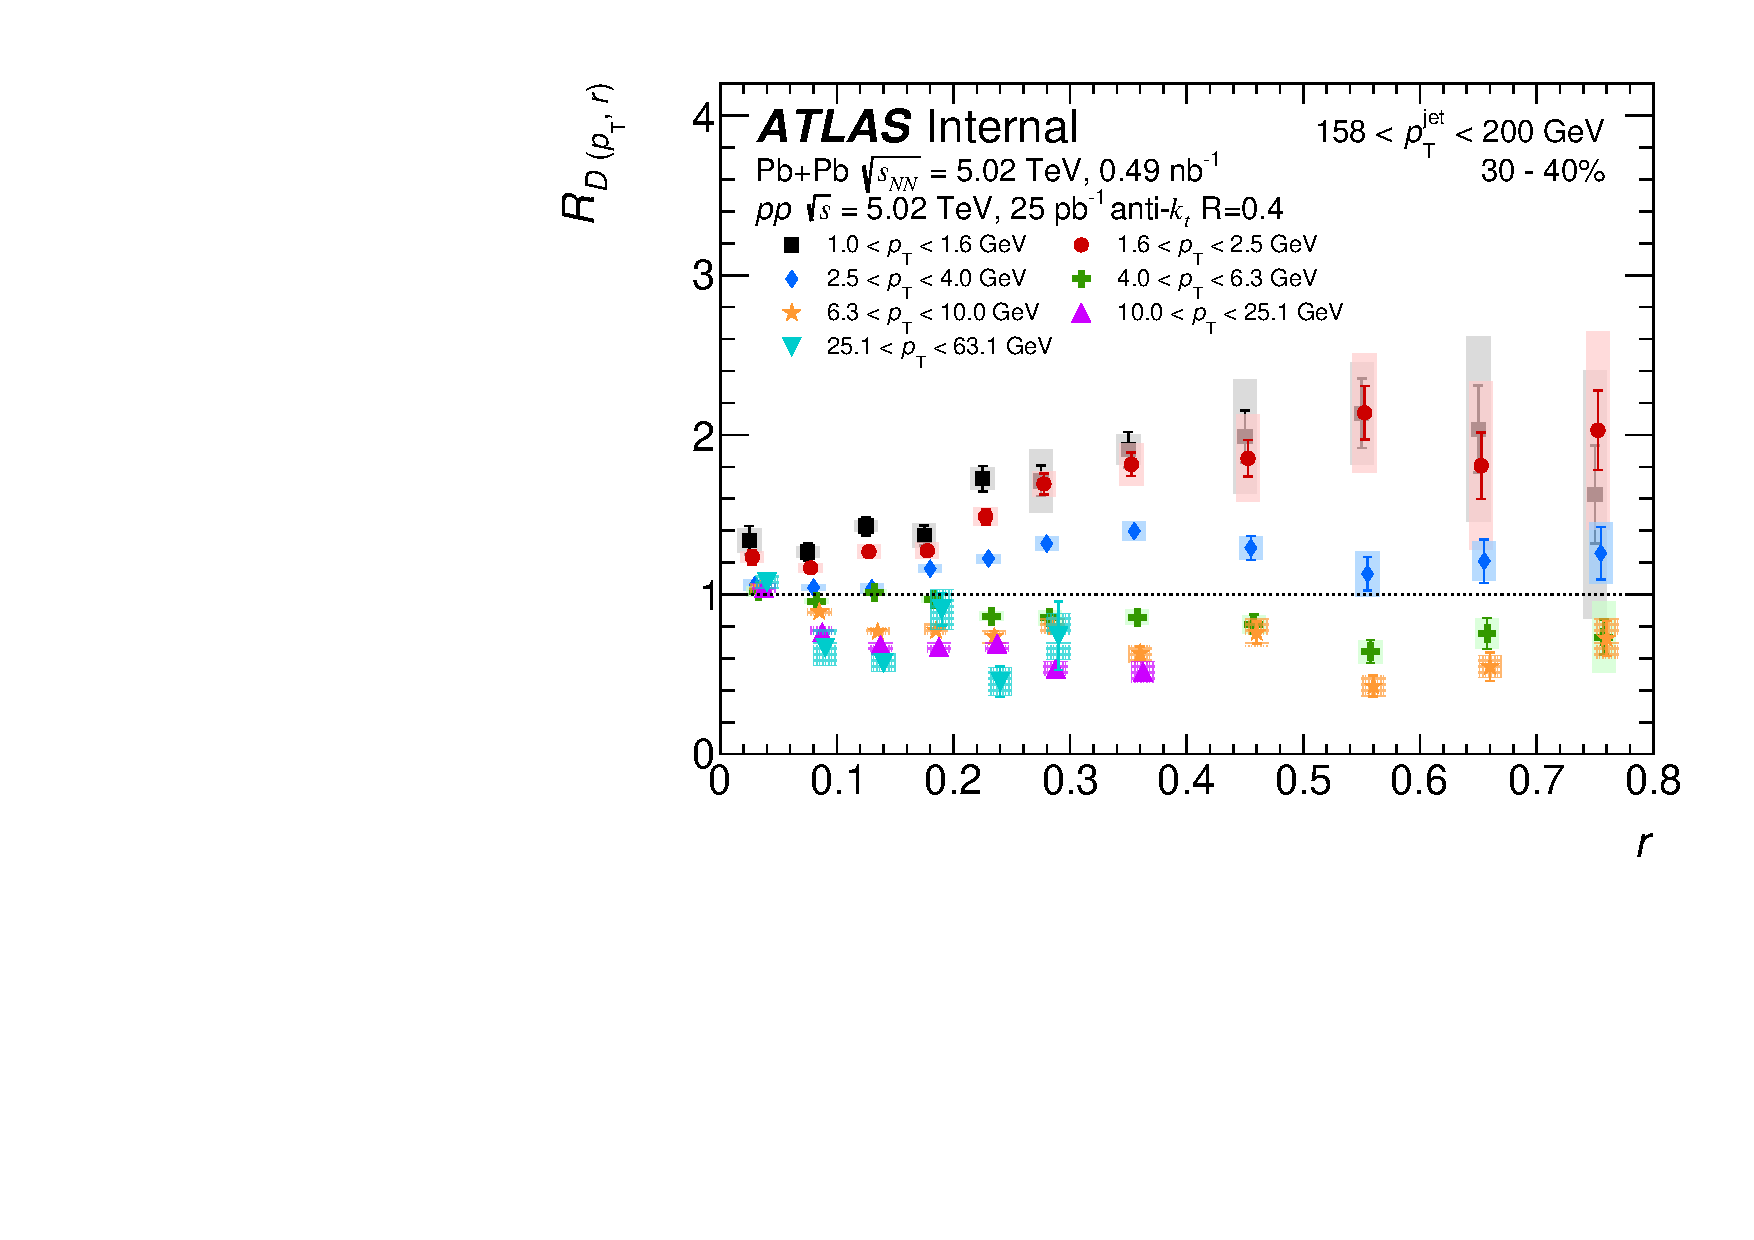
\includegraphics[width=0.48\textwidth]{figures/results/RDpT_dR_jet8_cent3} \\
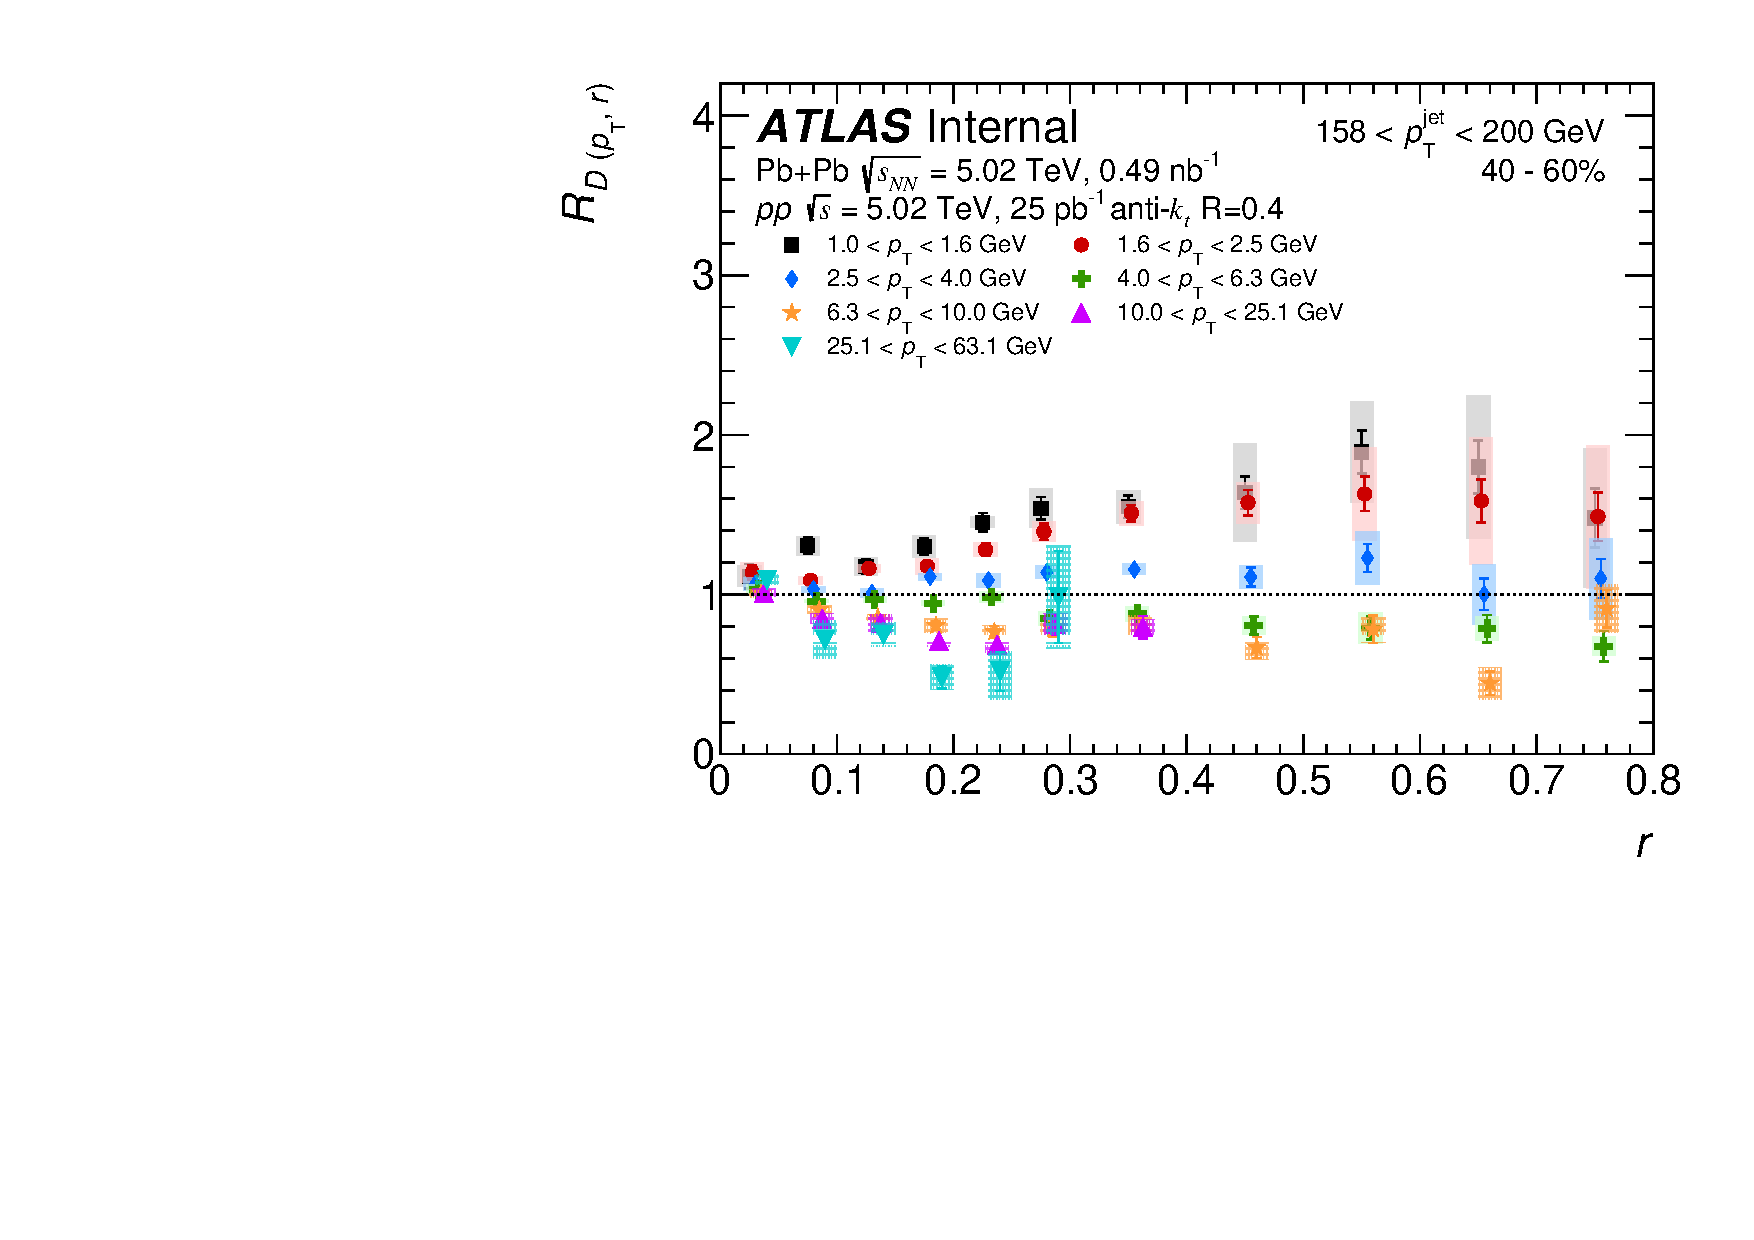
\includegraphics[width=0.48\textwidth]{figures/results/RDpT_dR_jet8_cent4} &
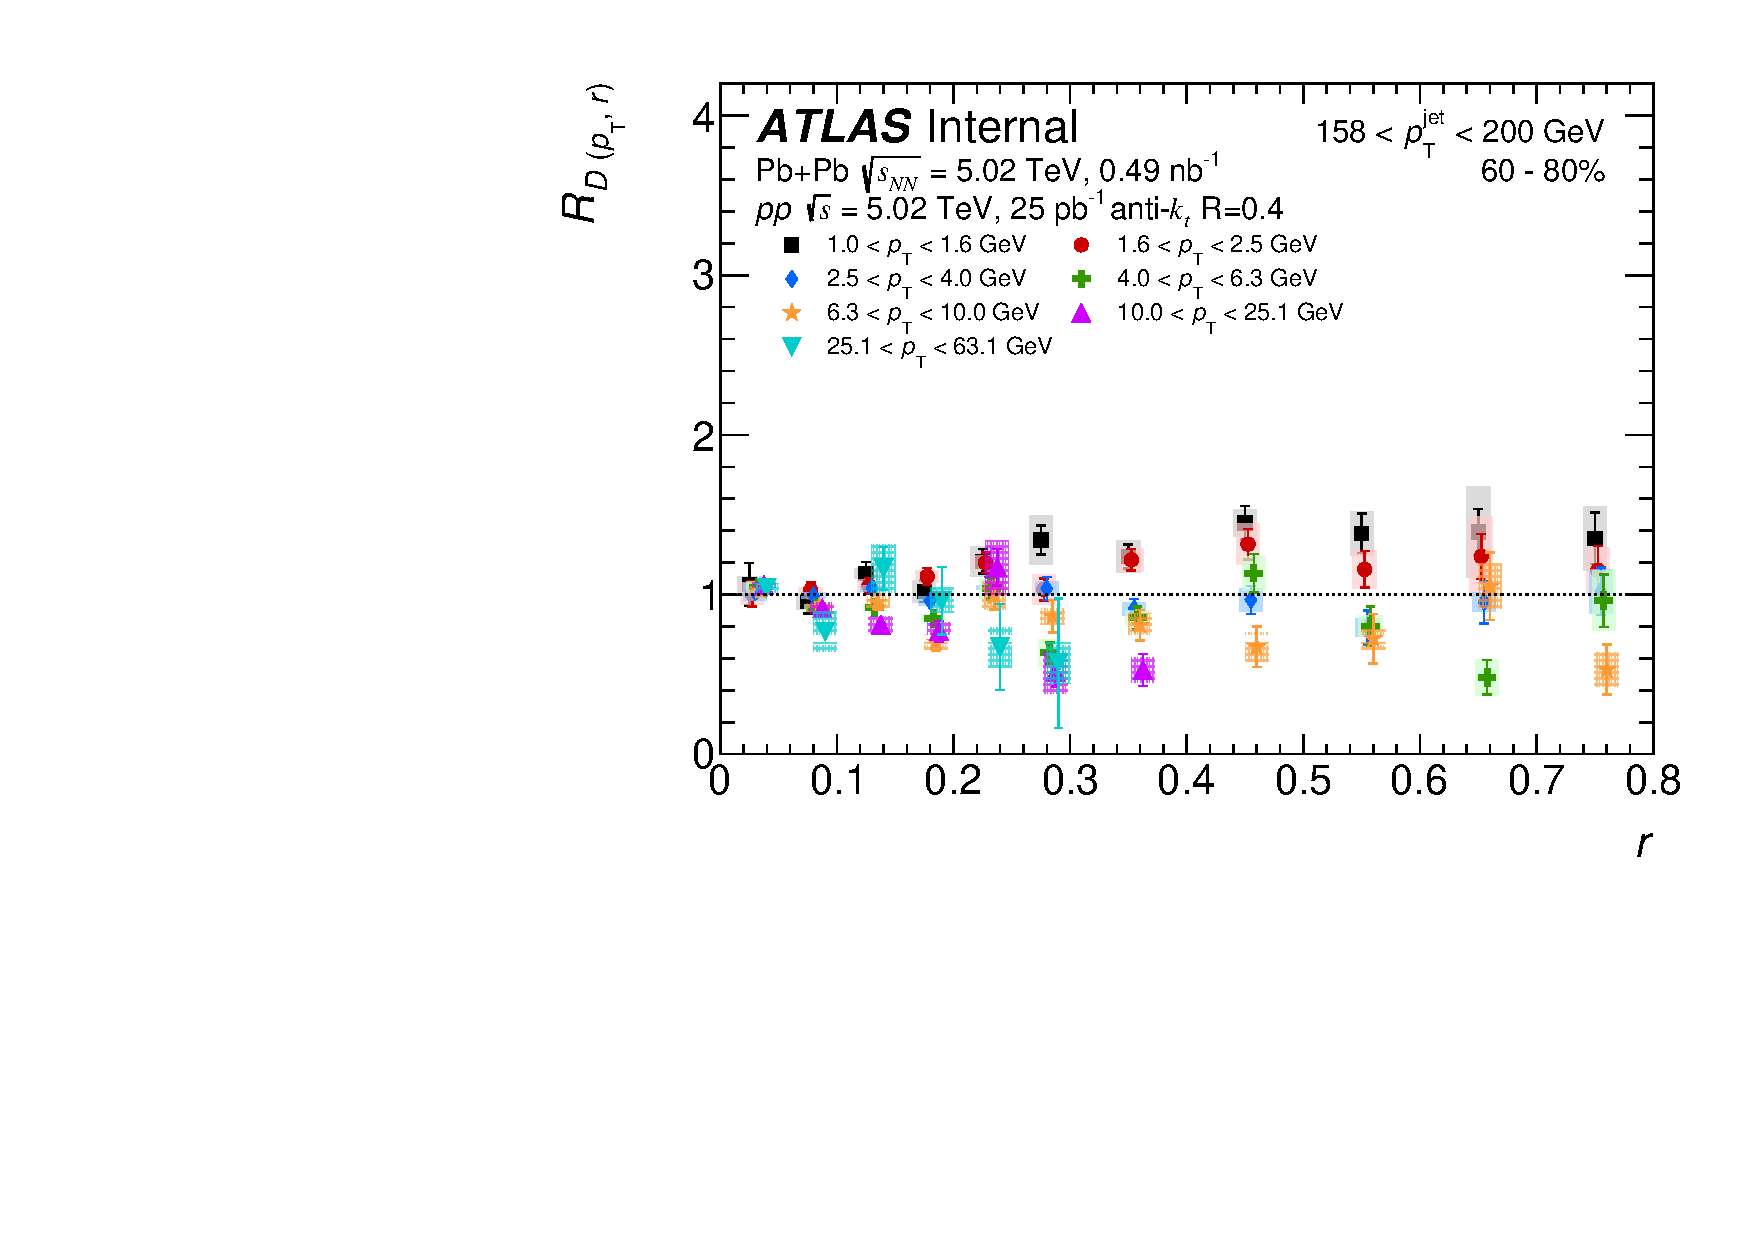
\includegraphics[width=0.48\textwidth]{figures/results/RDpT_dR_jet8_cent5} \\
\end{tabular}}
\caption{ The \RDptr\ distributions as a function of \rvar\ for different \pt\ selections in 158--200 GeV jets.
The different panels refer to different centrality selections.
The vertical bars on the data points indicate statistical uncertainties while the shaded boxes indicate systematic uncertainties.
The widths of the boxes are not indicative of the bin size and the points are shifted horizontally for better visibility.}
\label{fig:fullset_rptr_j8}
\end{figure}

\begin{figure}[h]
\centerline{
\begin{tabular}{ccc}
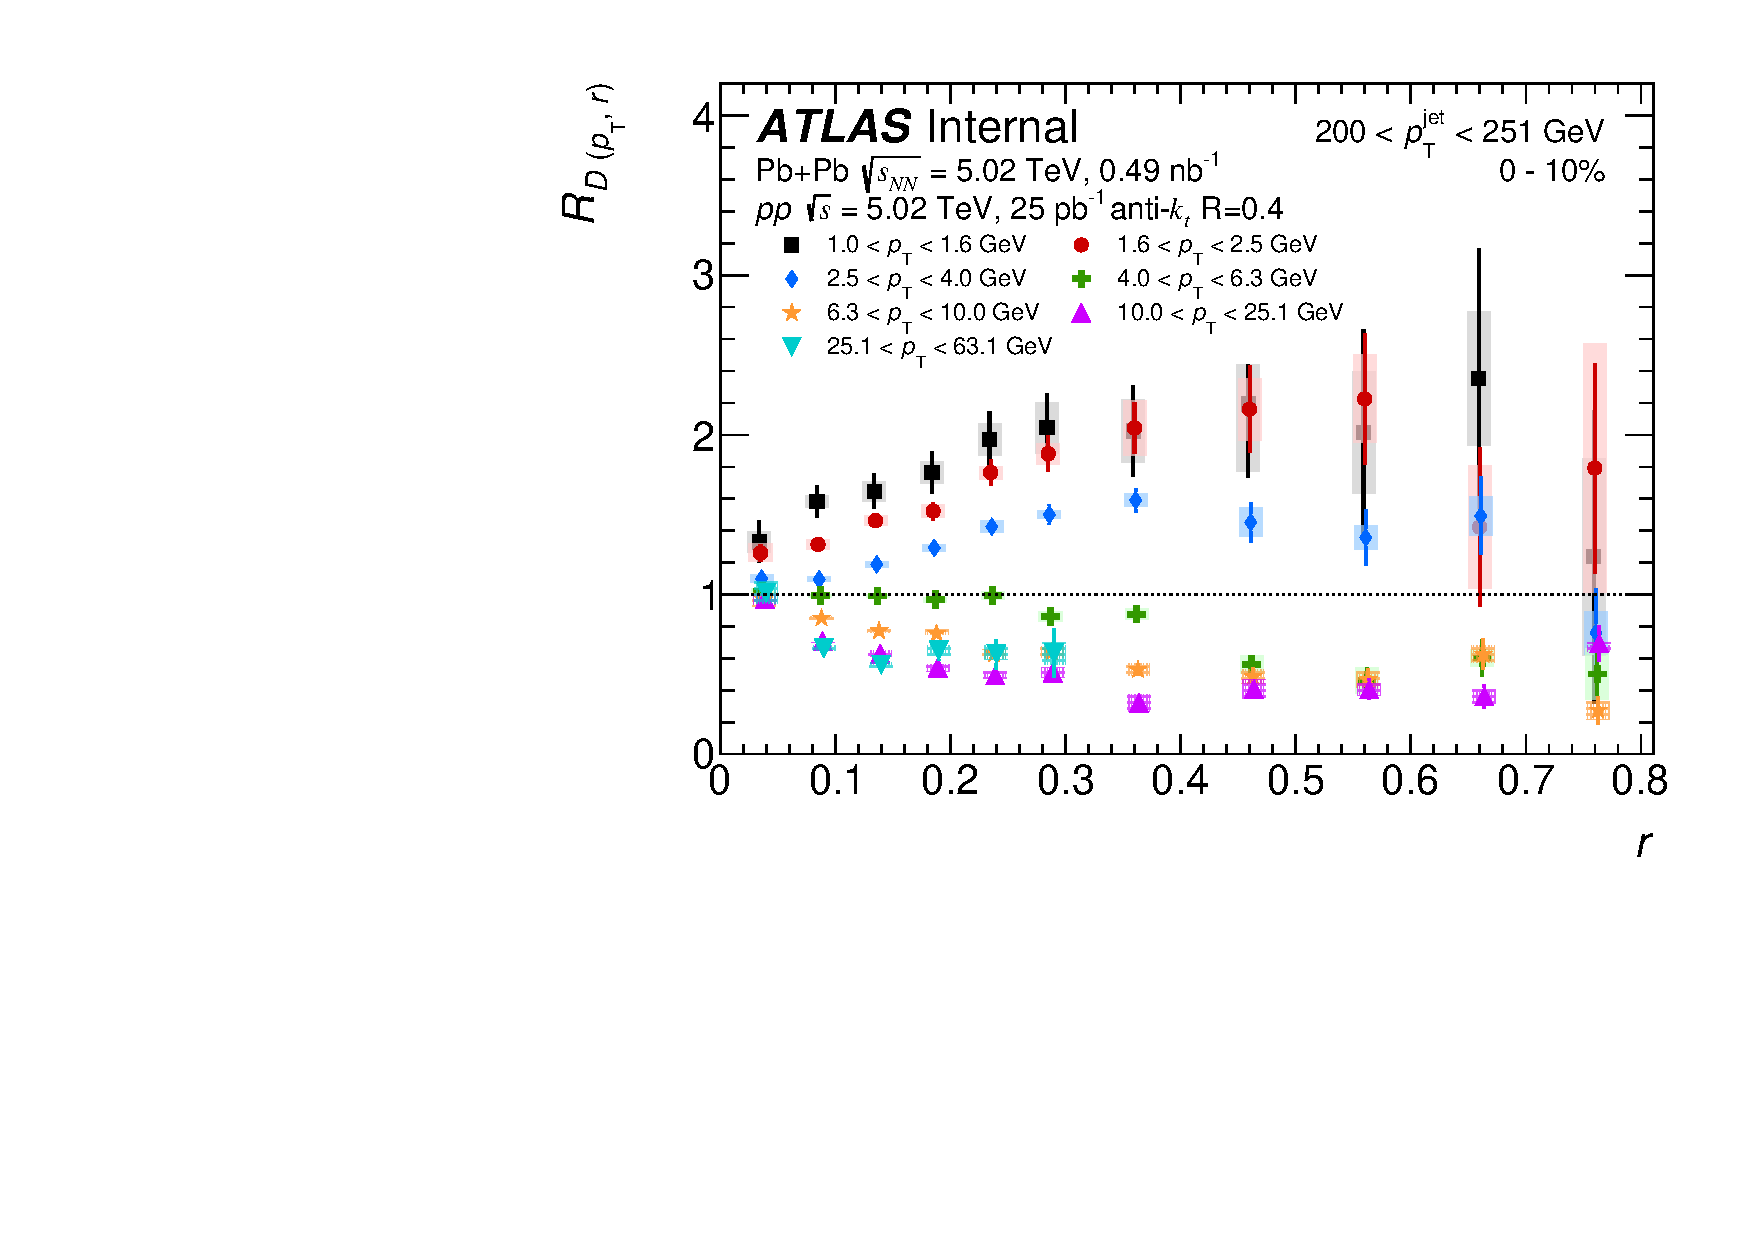
\includegraphics[width=0.48\textwidth]{figures/results/RDpT_dR_jet9_cent0} &
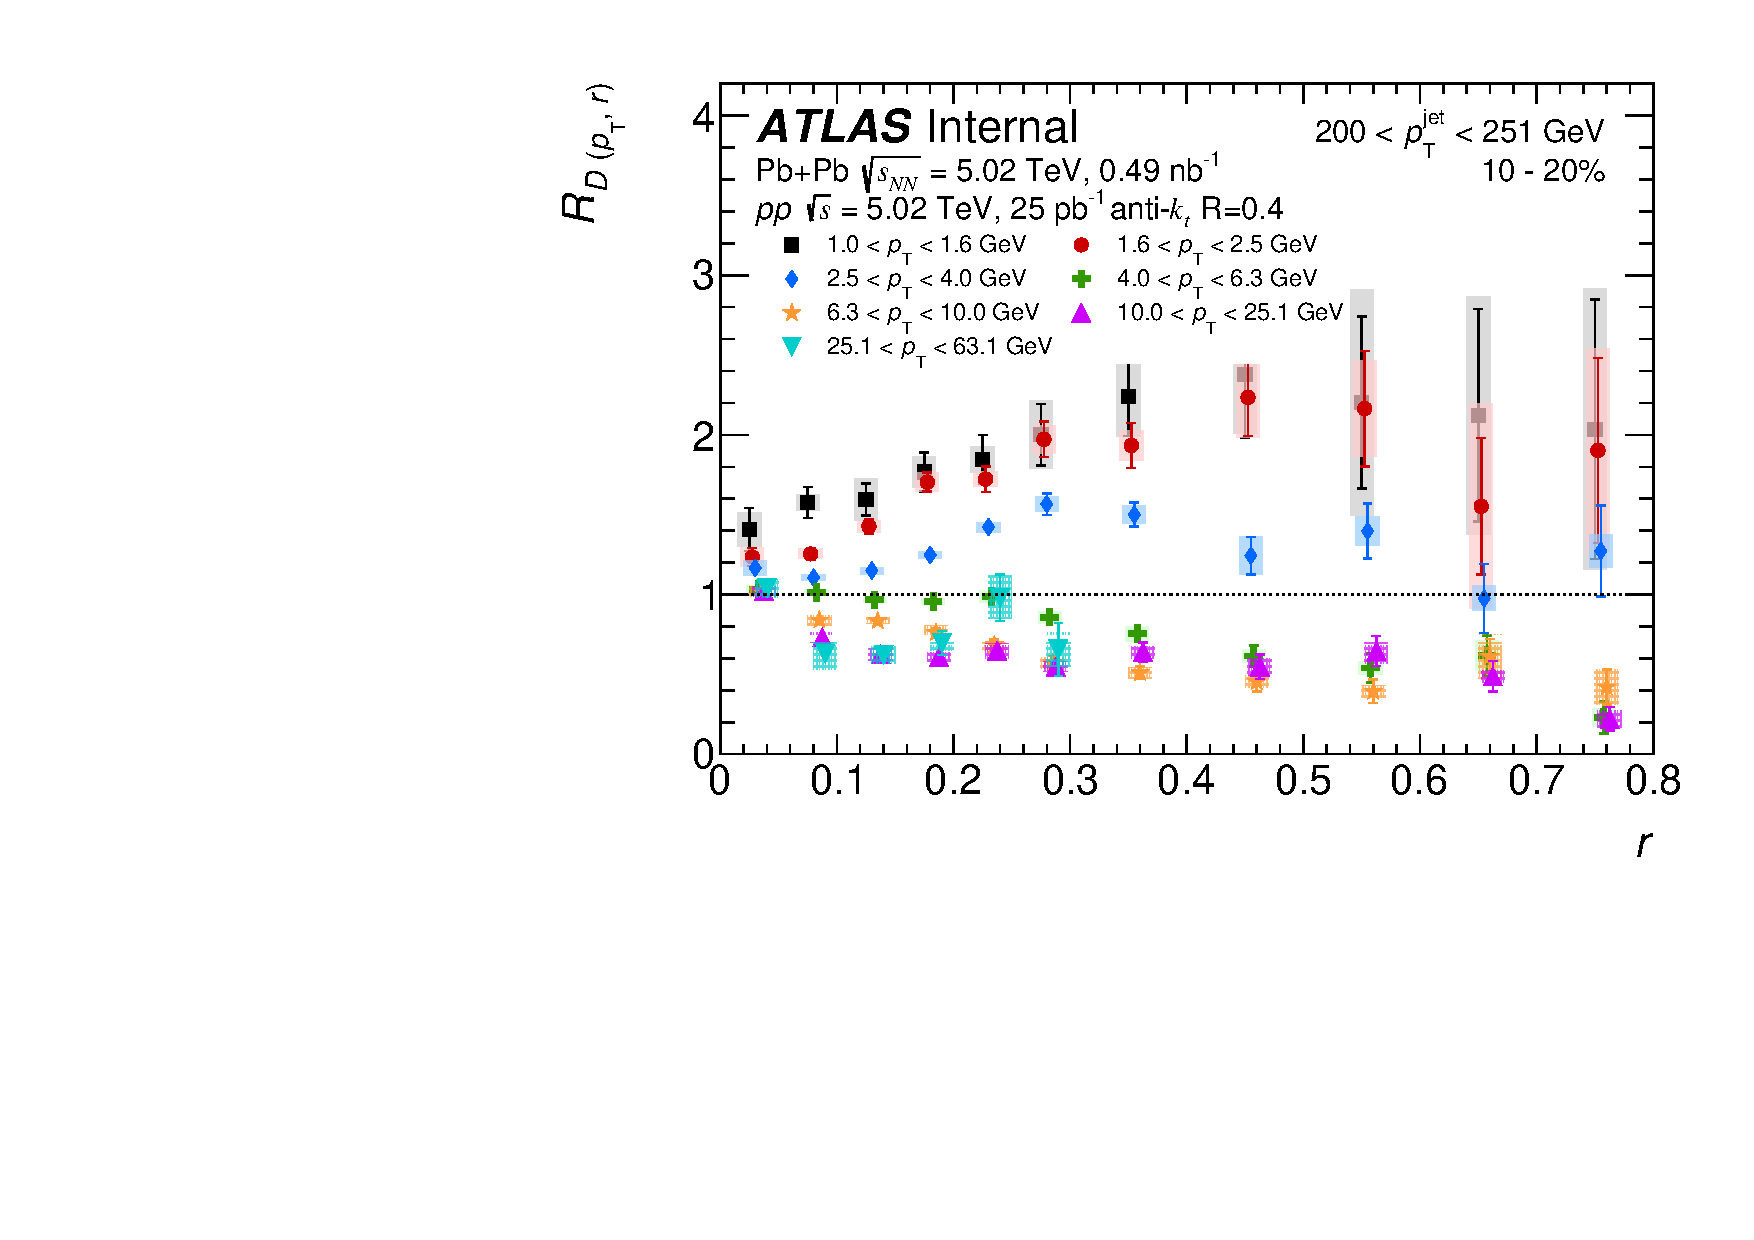
\includegraphics[width=0.48\textwidth]{figures/results/RDpT_dR_jet9_cent1} \\
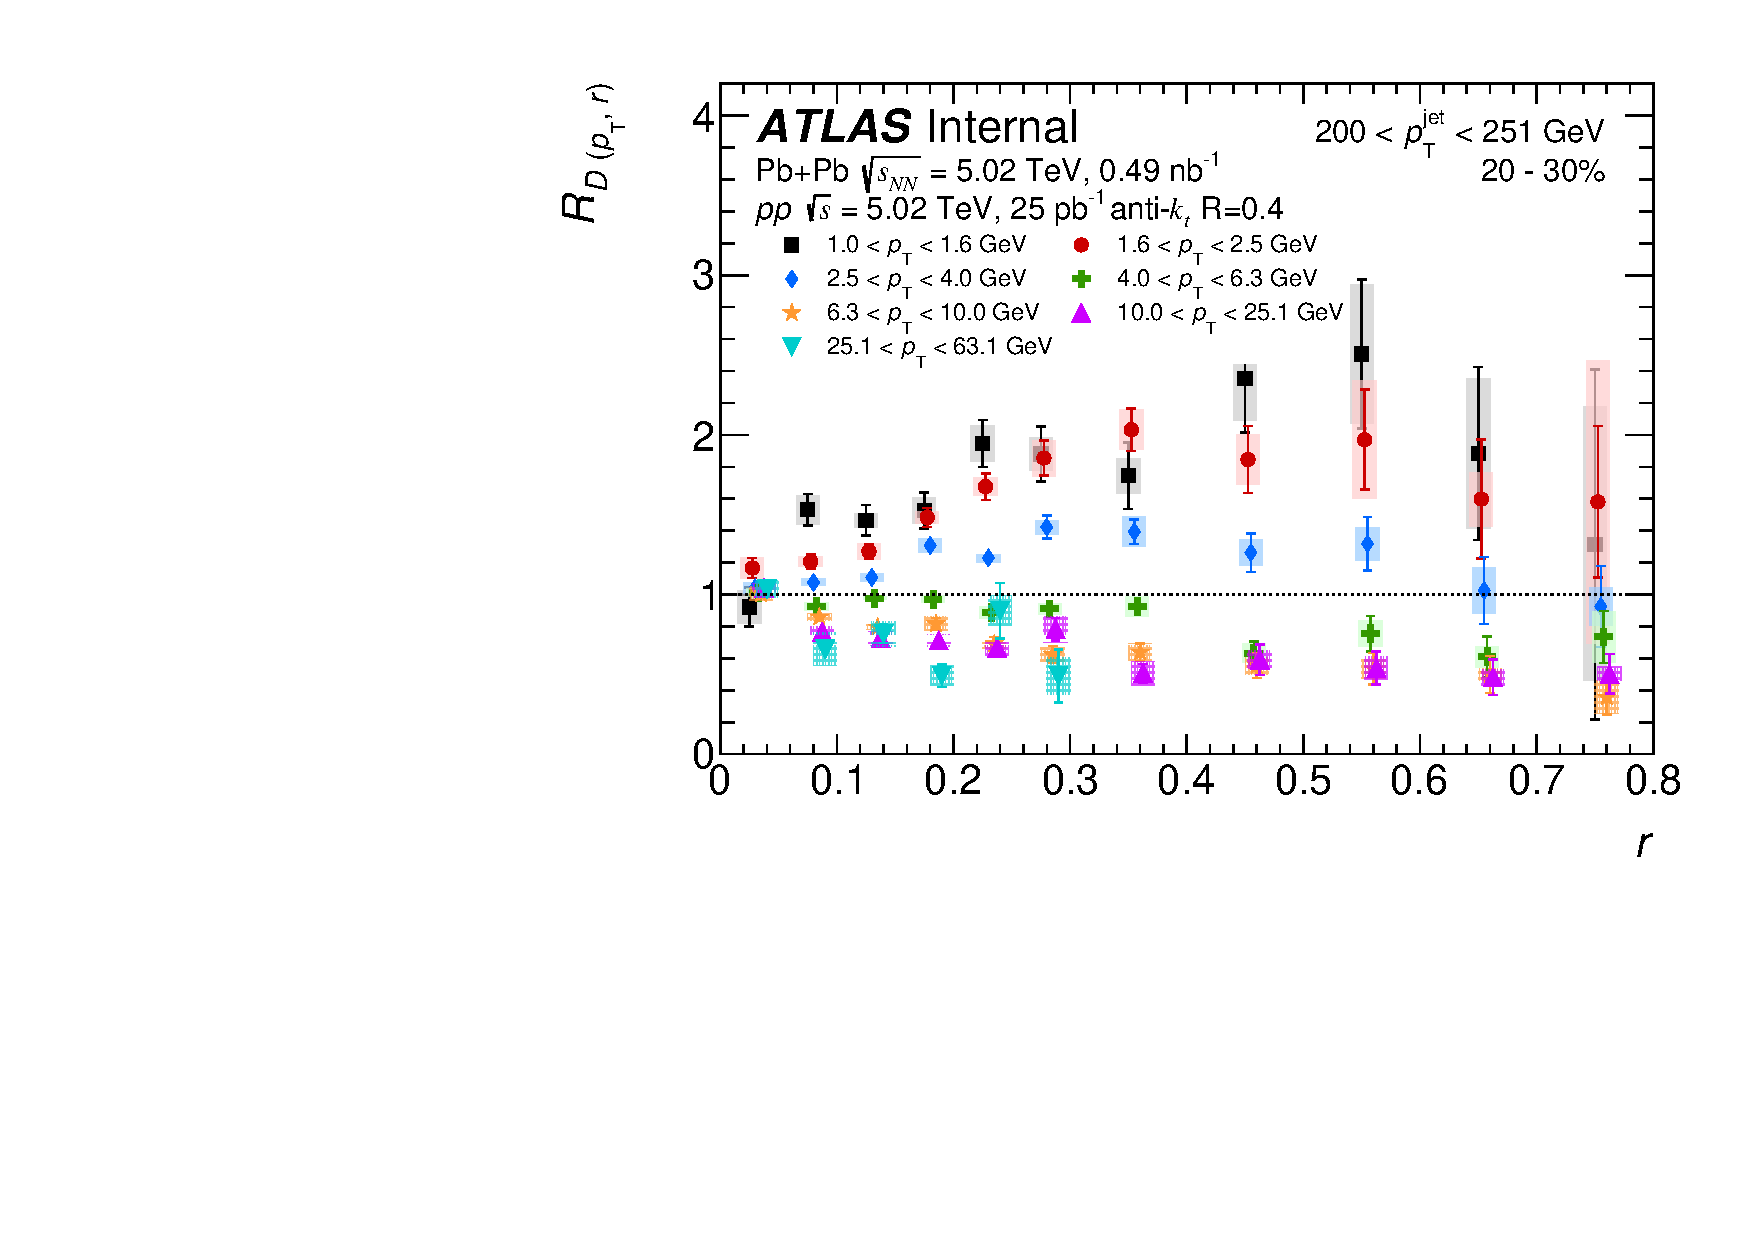
\includegraphics[width=0.48\textwidth]{figures/results/RDpT_dR_jet9_cent2} &
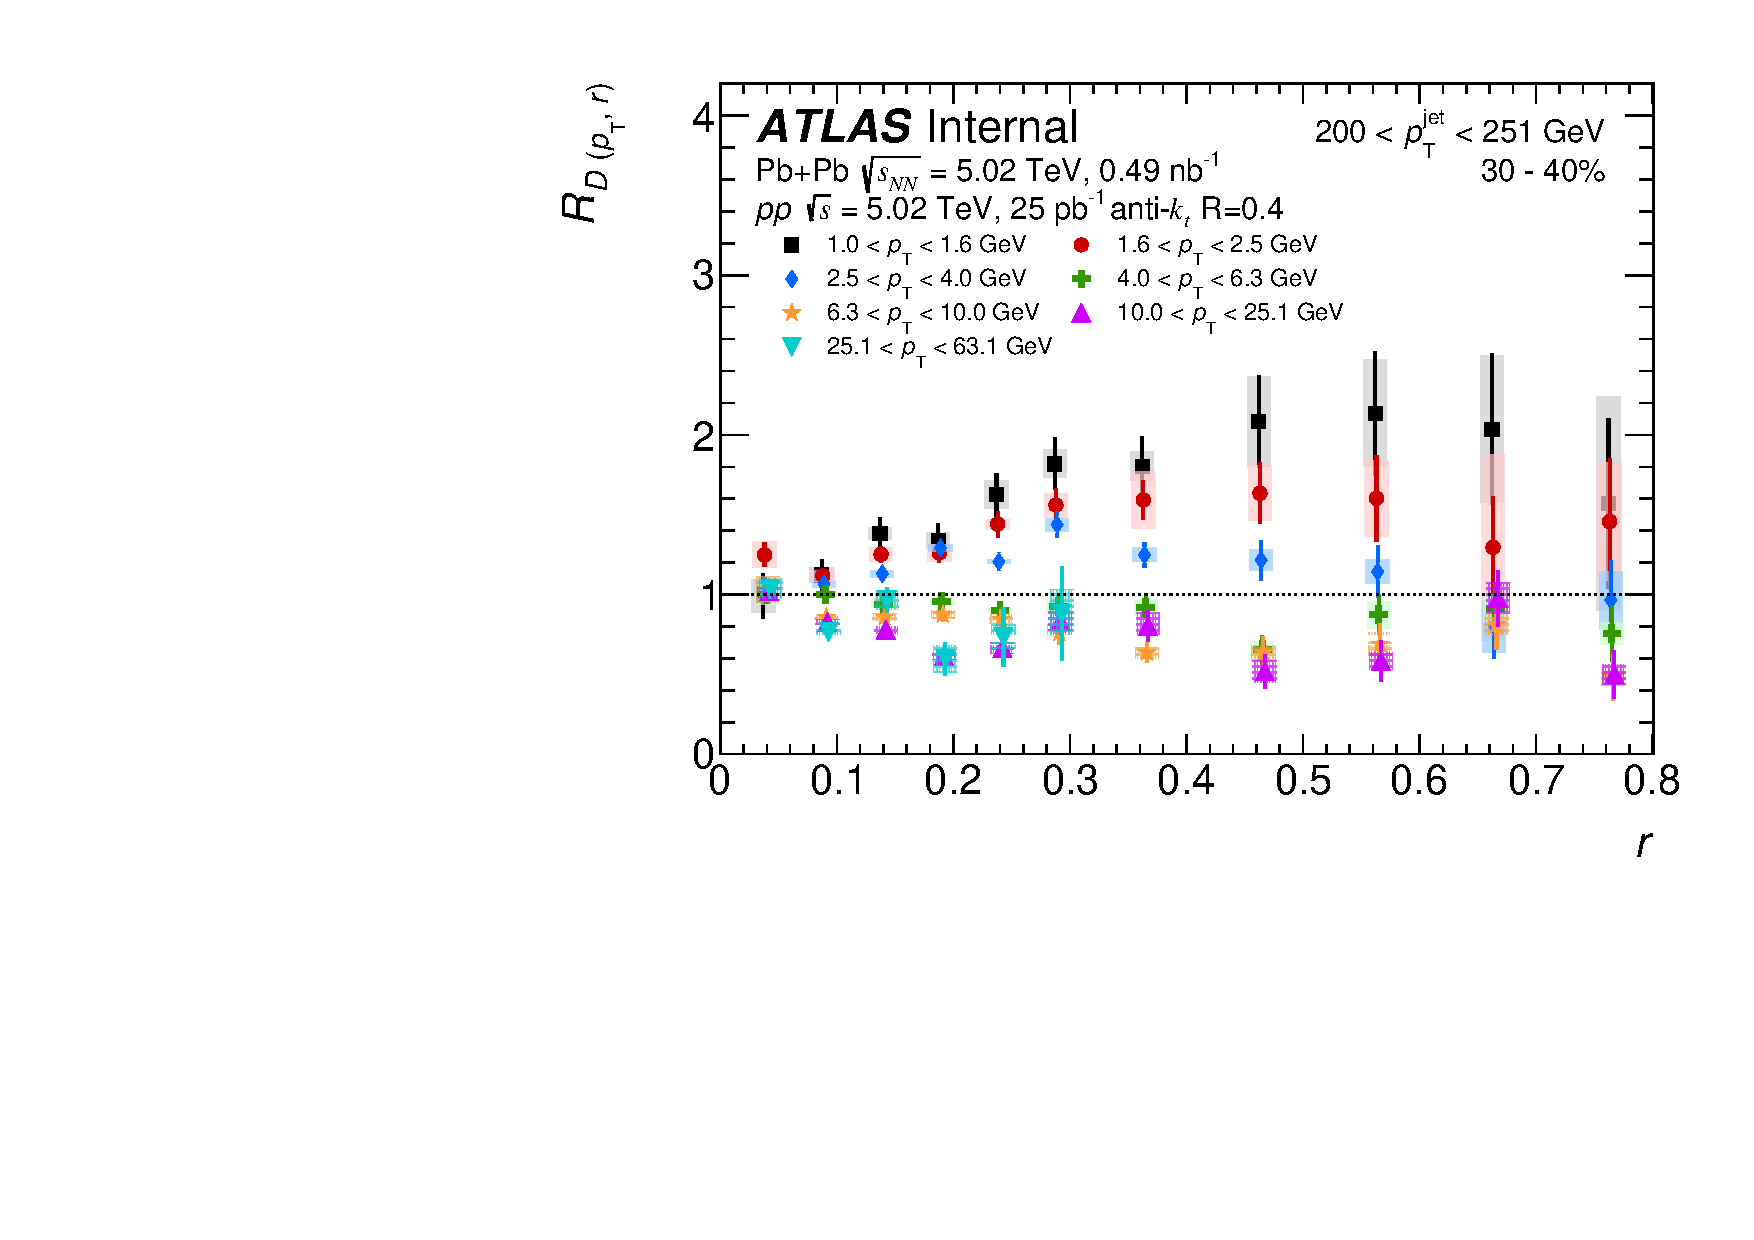
\includegraphics[width=0.48\textwidth]{figures/results/RDpT_dR_jet9_cent3} \\
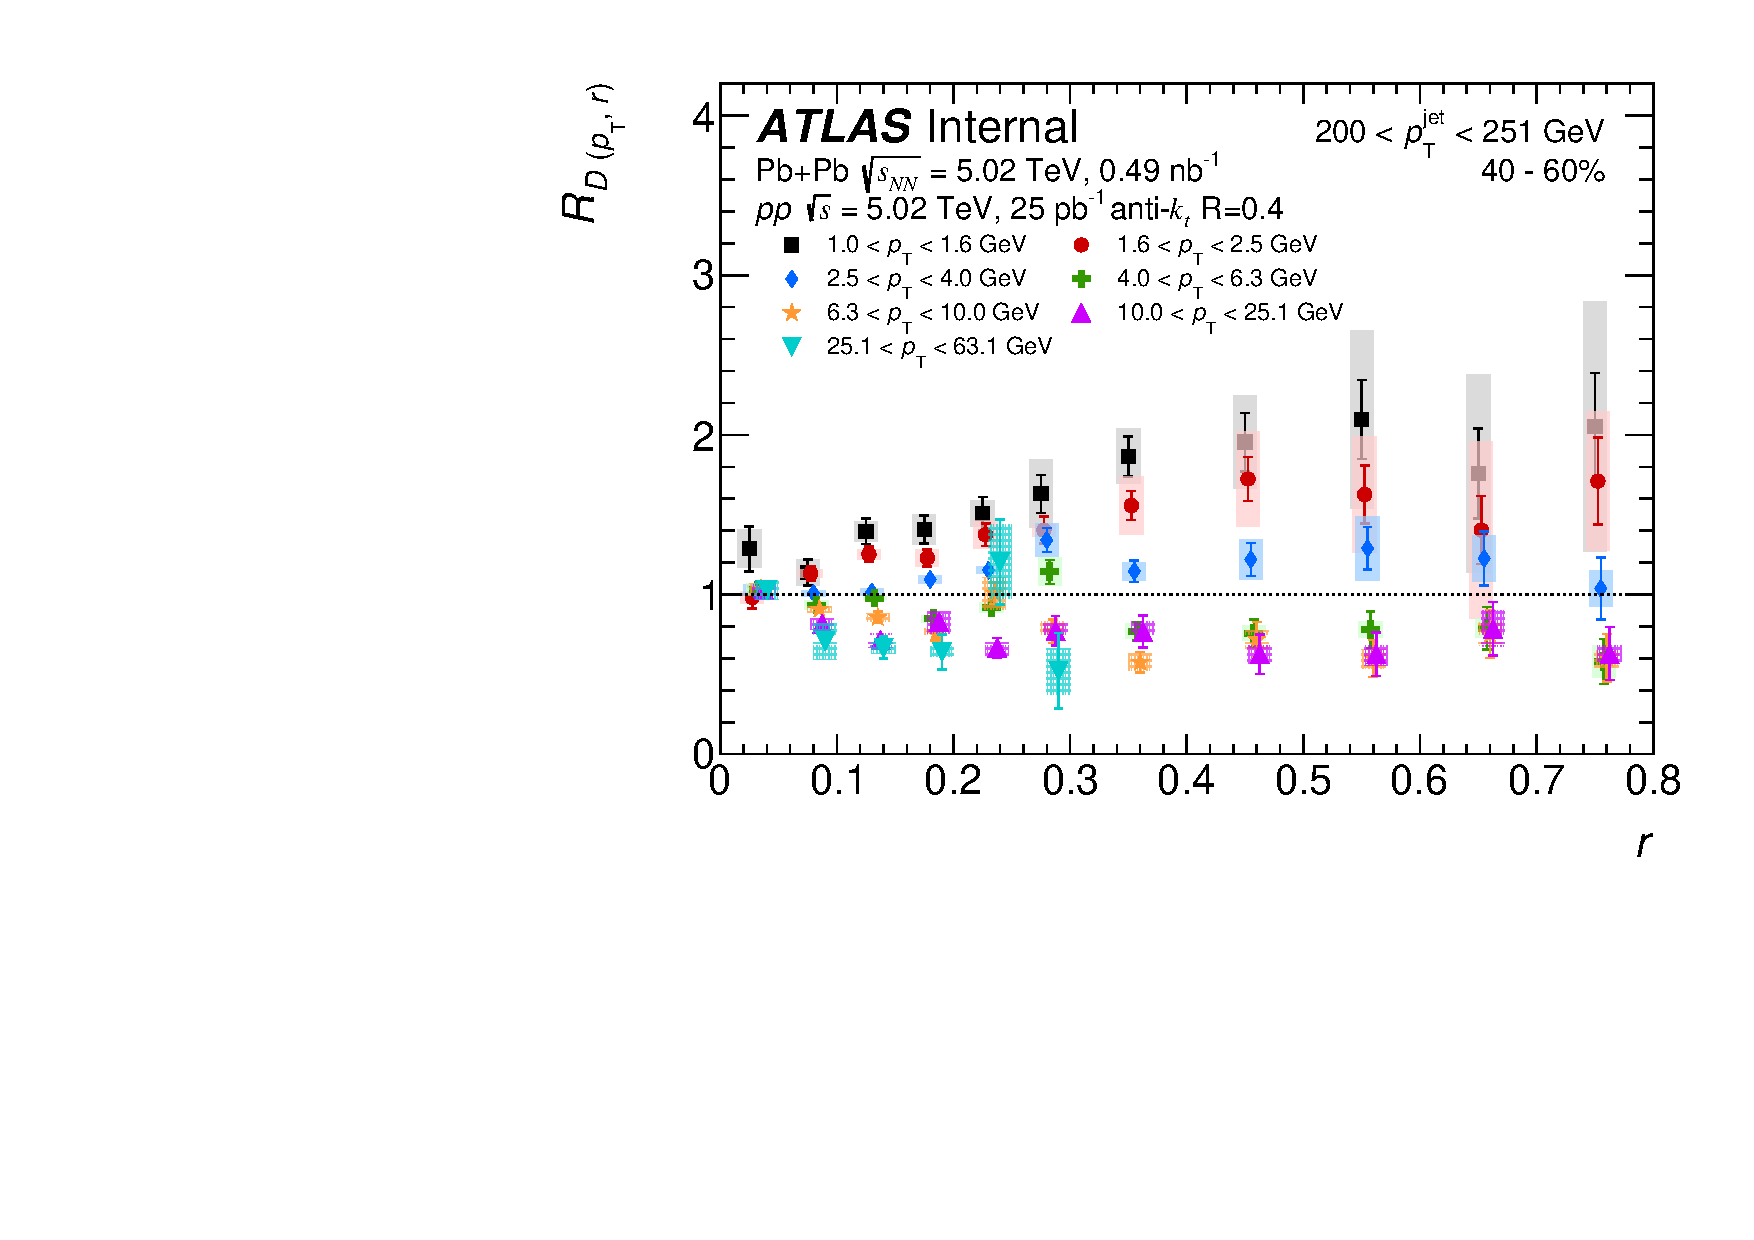
\includegraphics[width=0.48\textwidth]{figures/results/RDpT_dR_jet9_cent4} &
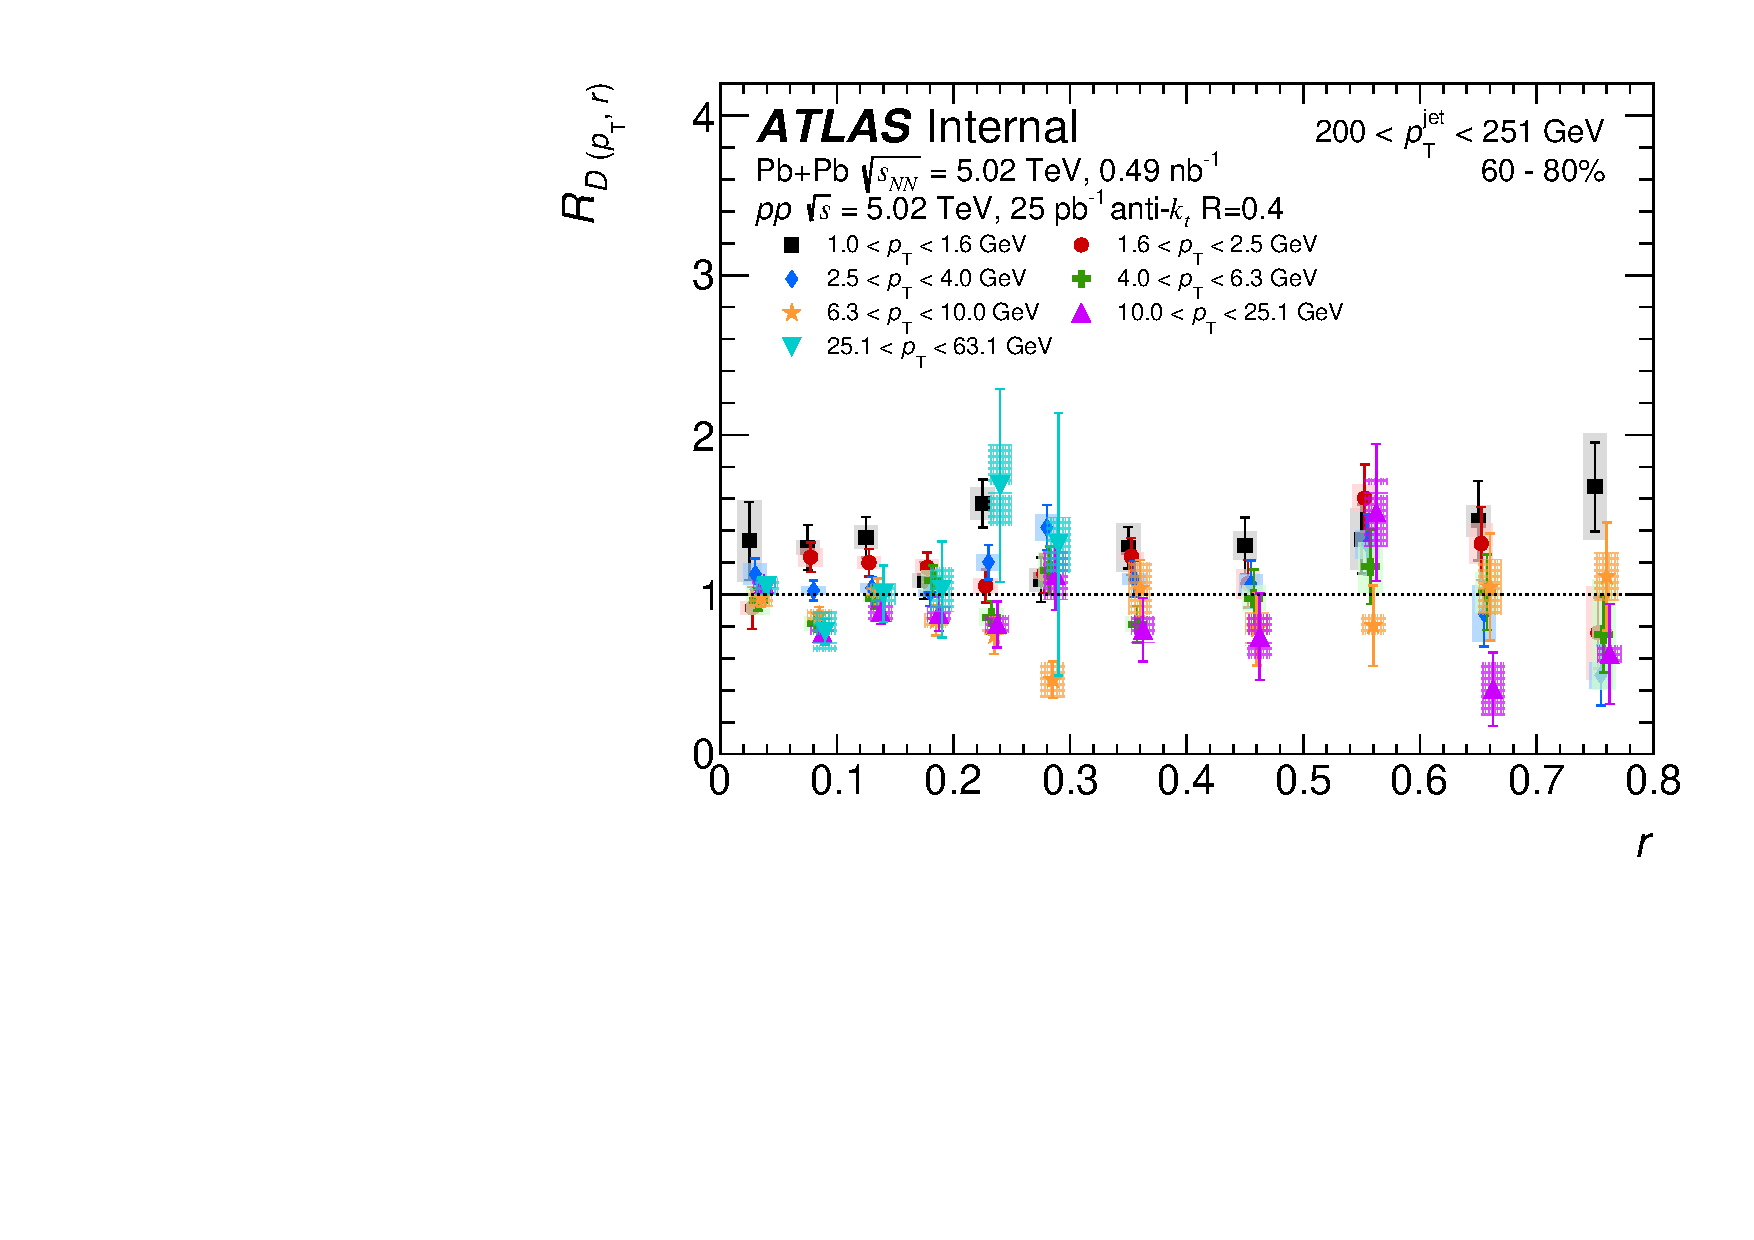
\includegraphics[width=0.48\textwidth]{figures/results/RDpT_dR_jet9_cent5} \\
\end{tabular}}
\caption{ The \RDptr\ distributions as a function of \rvar\ for different \pt\ selections in 200--251 GeV jets.
The different panels refer to different centrality selections.
The vertical bars on the data points indicate statistical uncertainties while the shaded boxes indicate systematic uncertainties.
The widths of the boxes are not indicative of the bin size and the points are shifted horizontally for better visibility.}
\label{fig:fullset_rptr_j9}
\end{figure}

\begin{figure}[h]
\centerline{
\begin{tabular}{ccc}
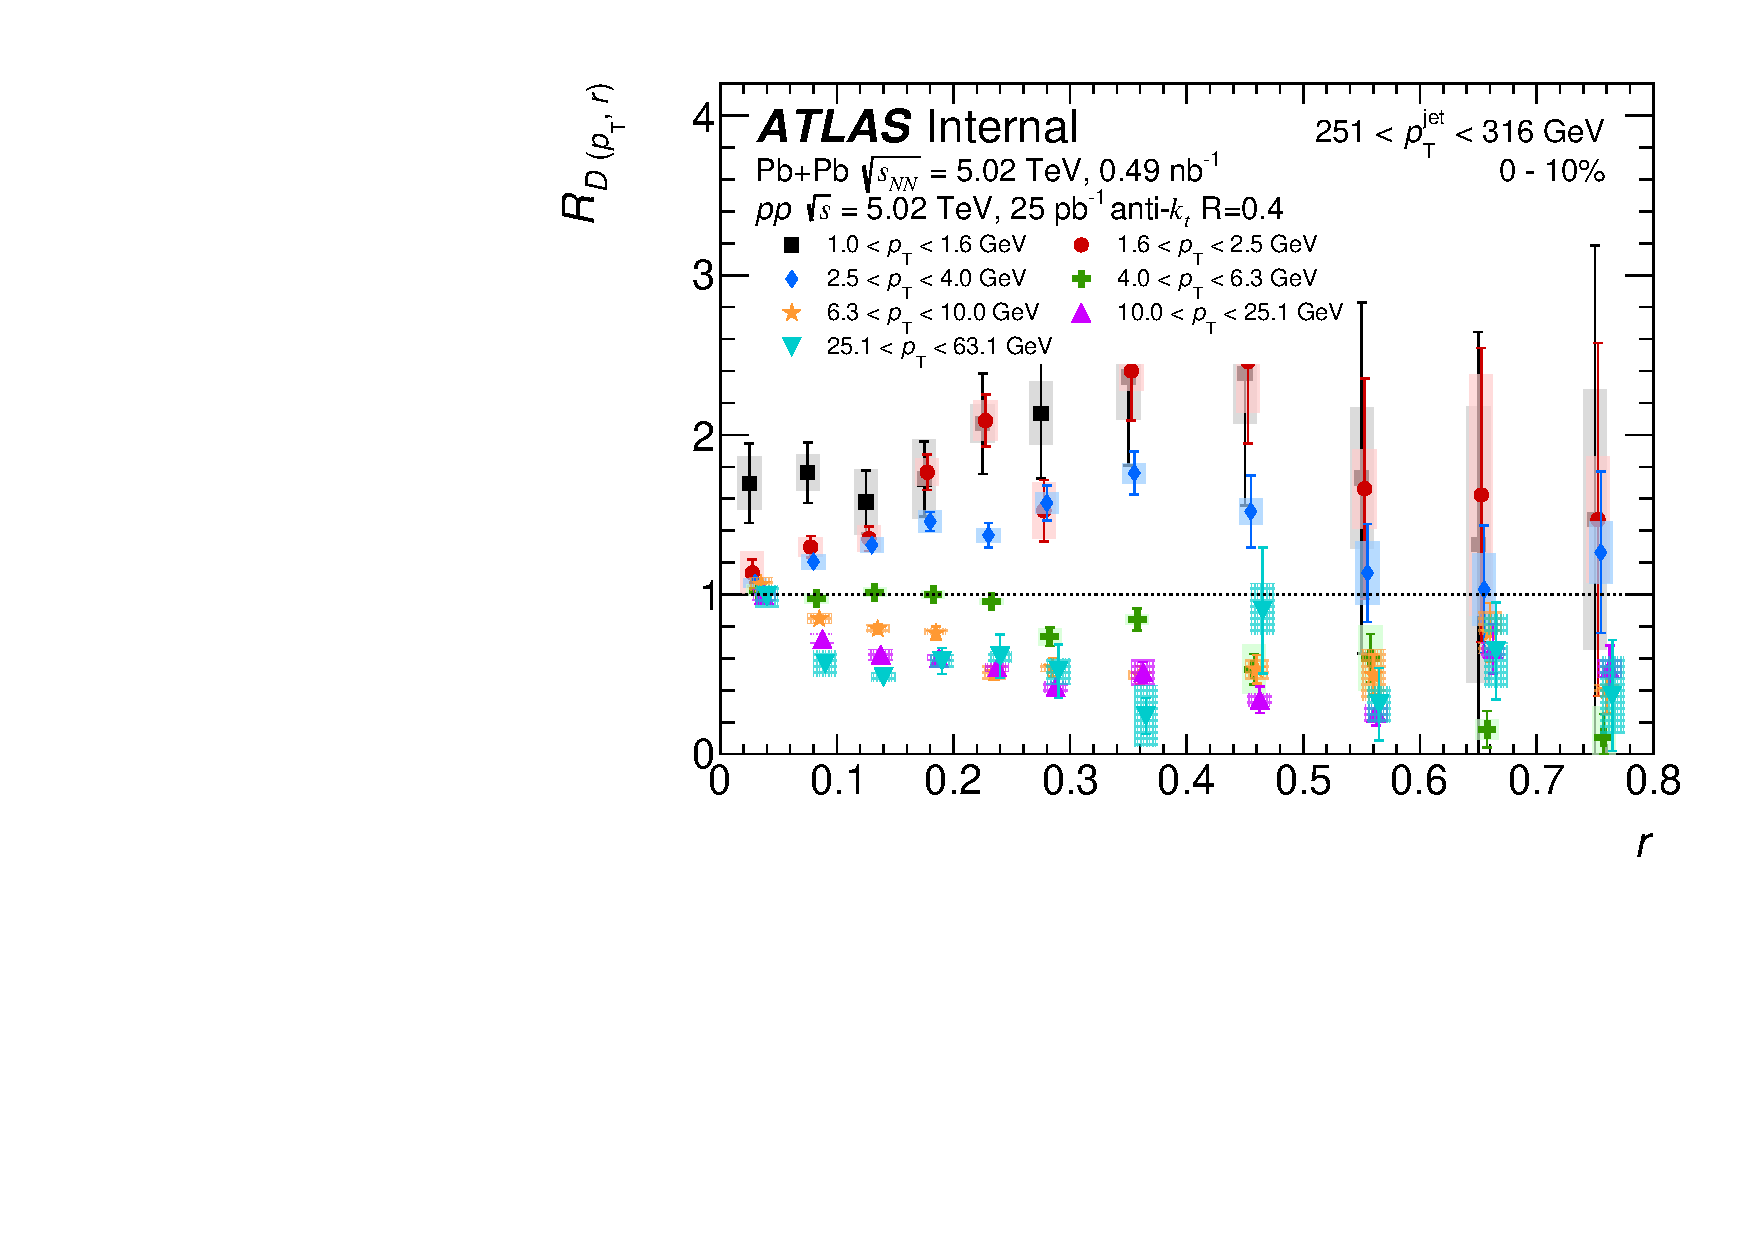
\includegraphics[width=0.48\textwidth]{figures/results/RDpT_dR_jet10_cent0} &
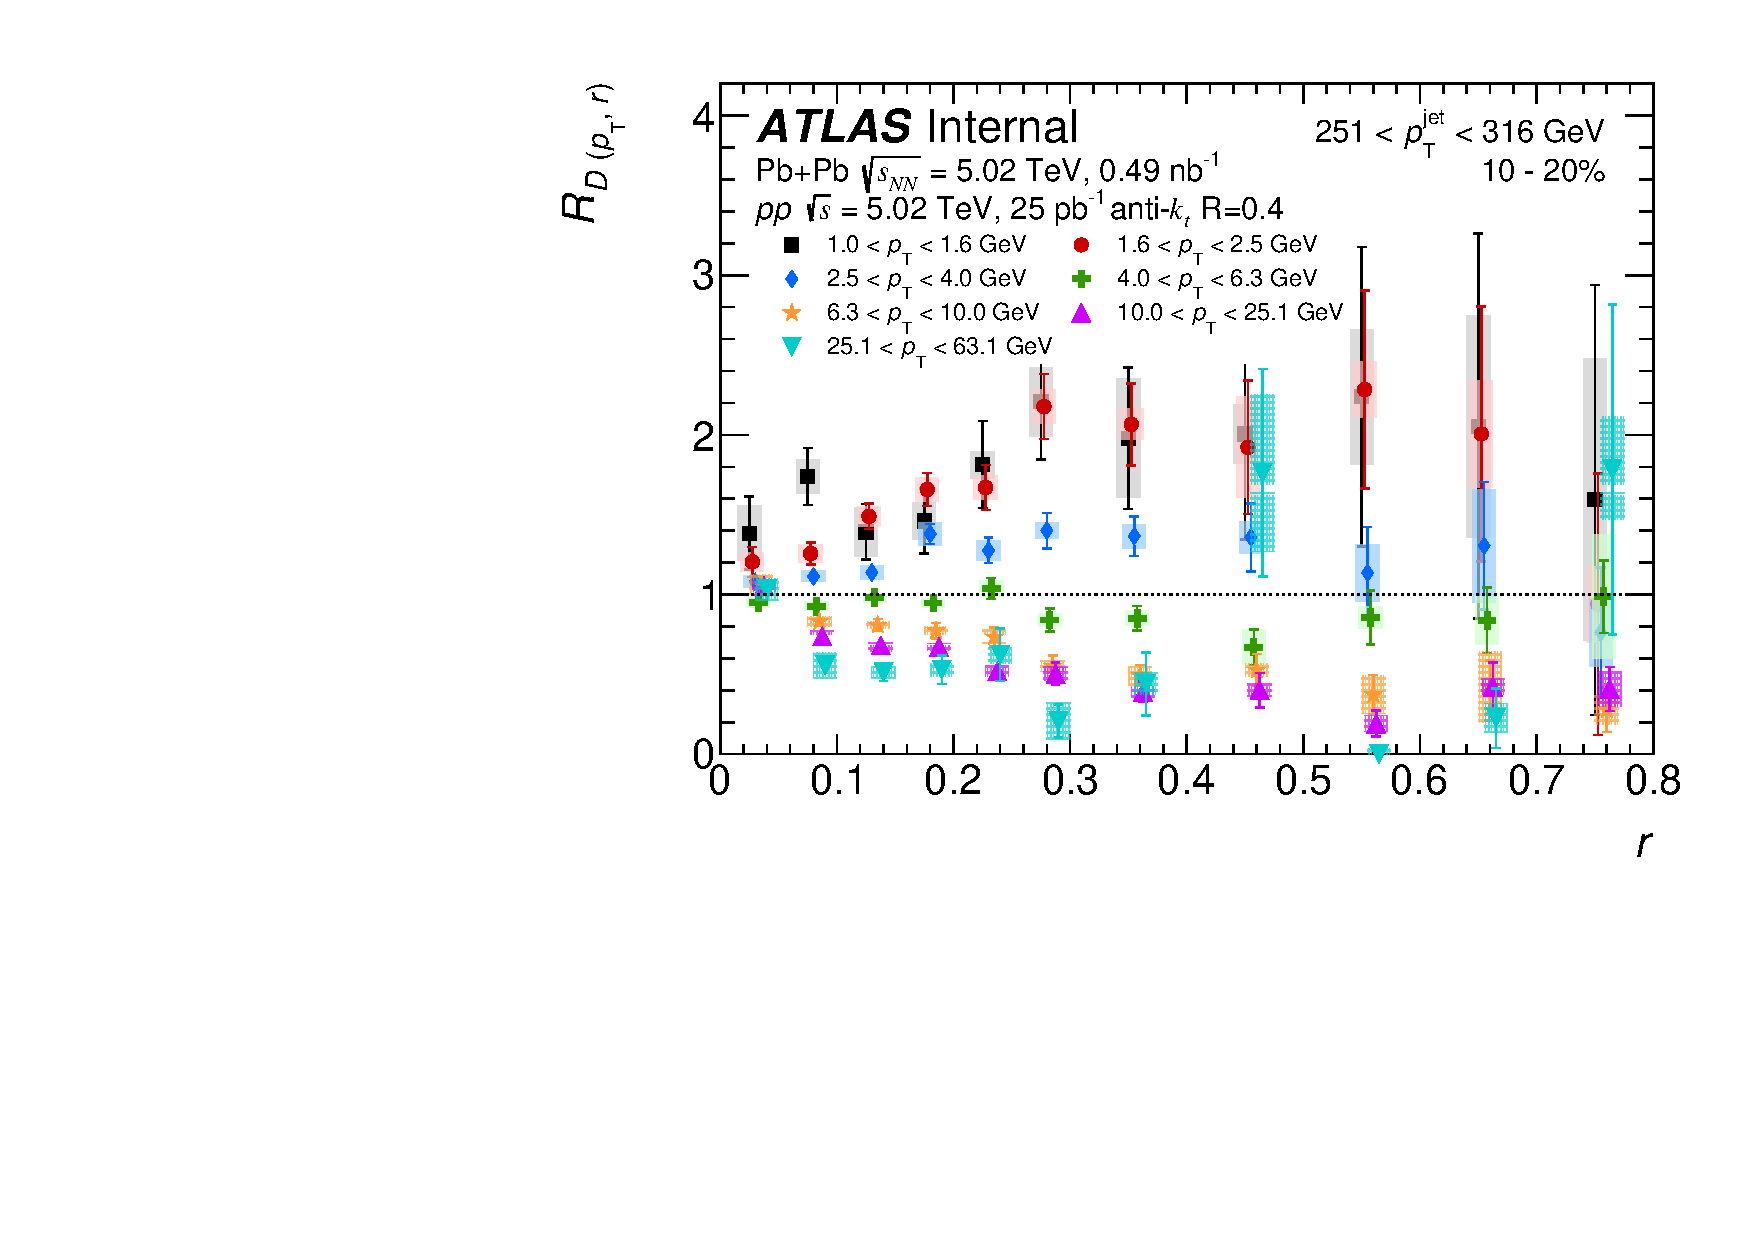
\includegraphics[width=0.48\textwidth]{figures/results/RDpT_dR_jet10_cent1} \\
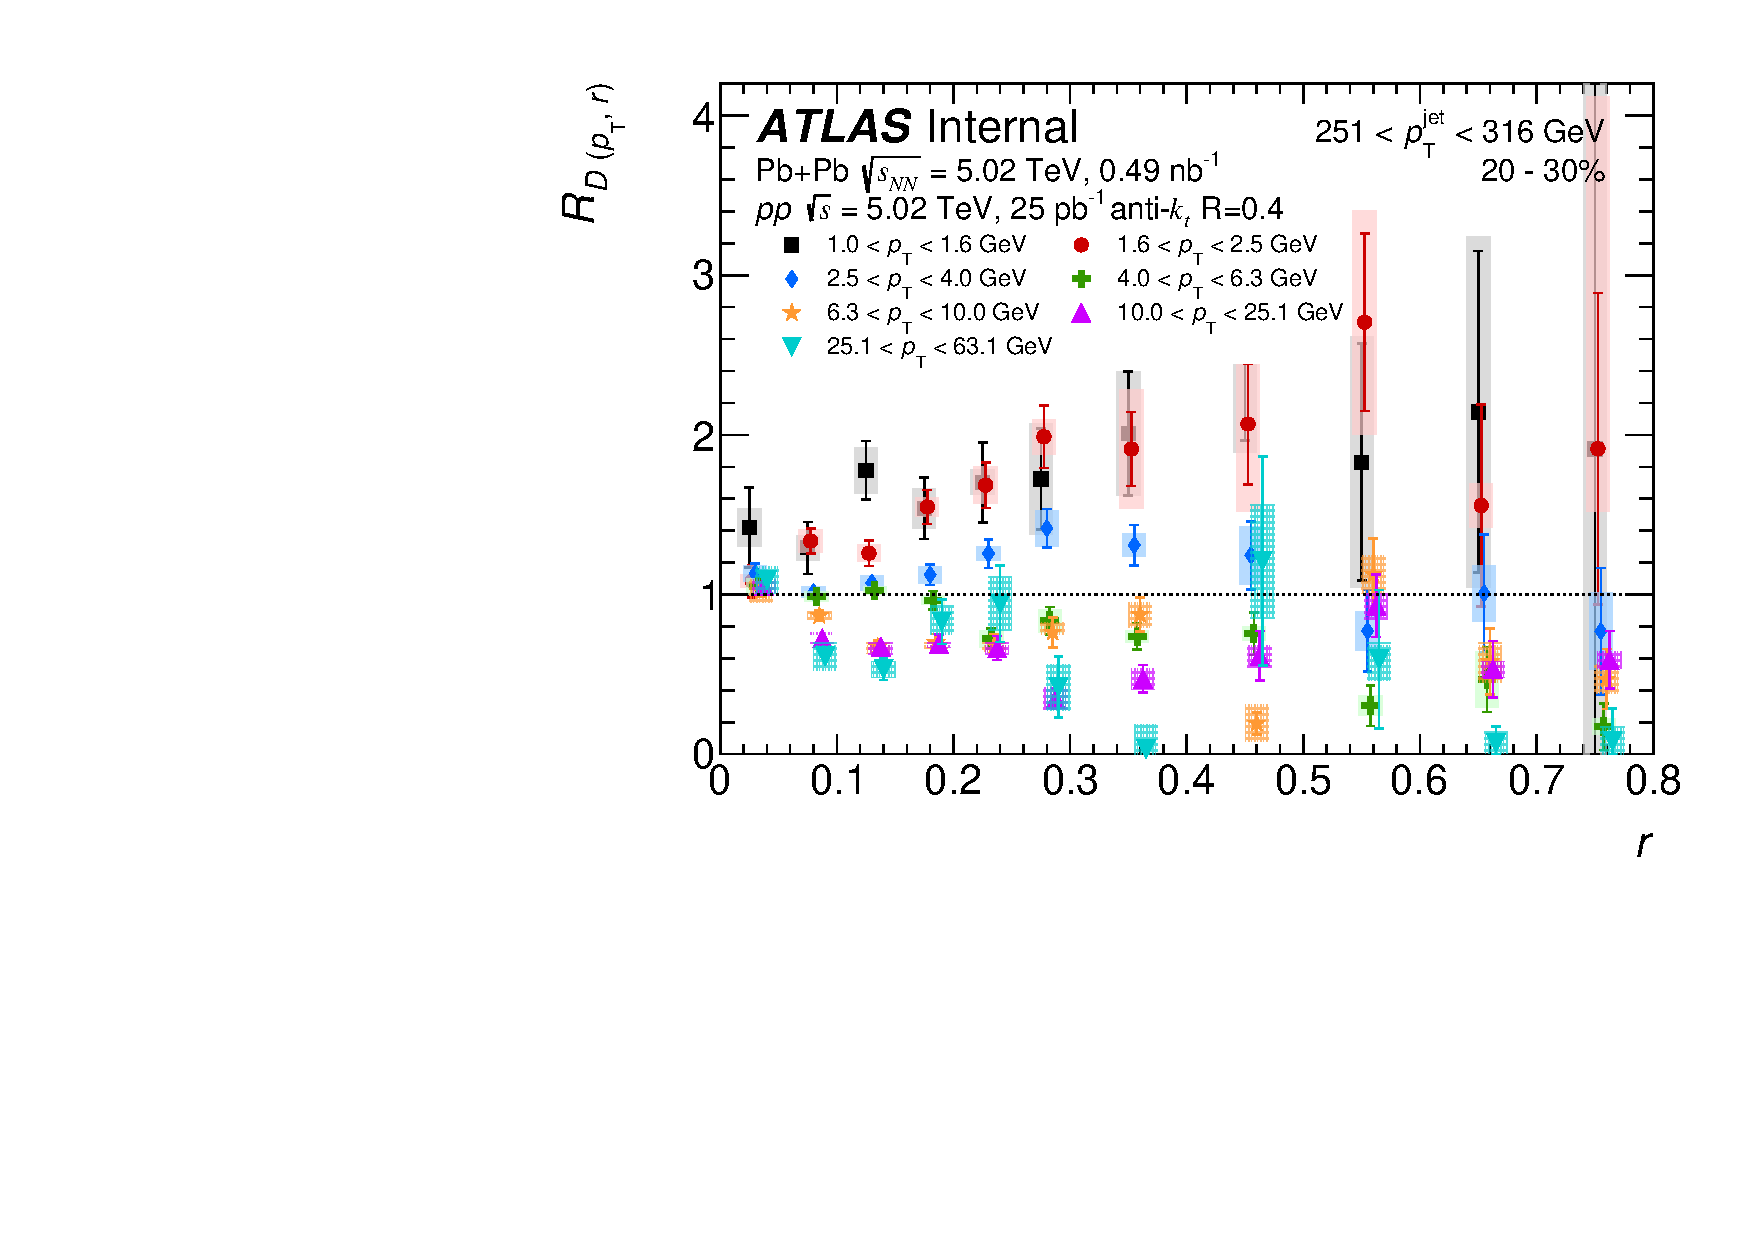
\includegraphics[width=0.48\textwidth]{figures/results/RDpT_dR_jet10_cent2} &
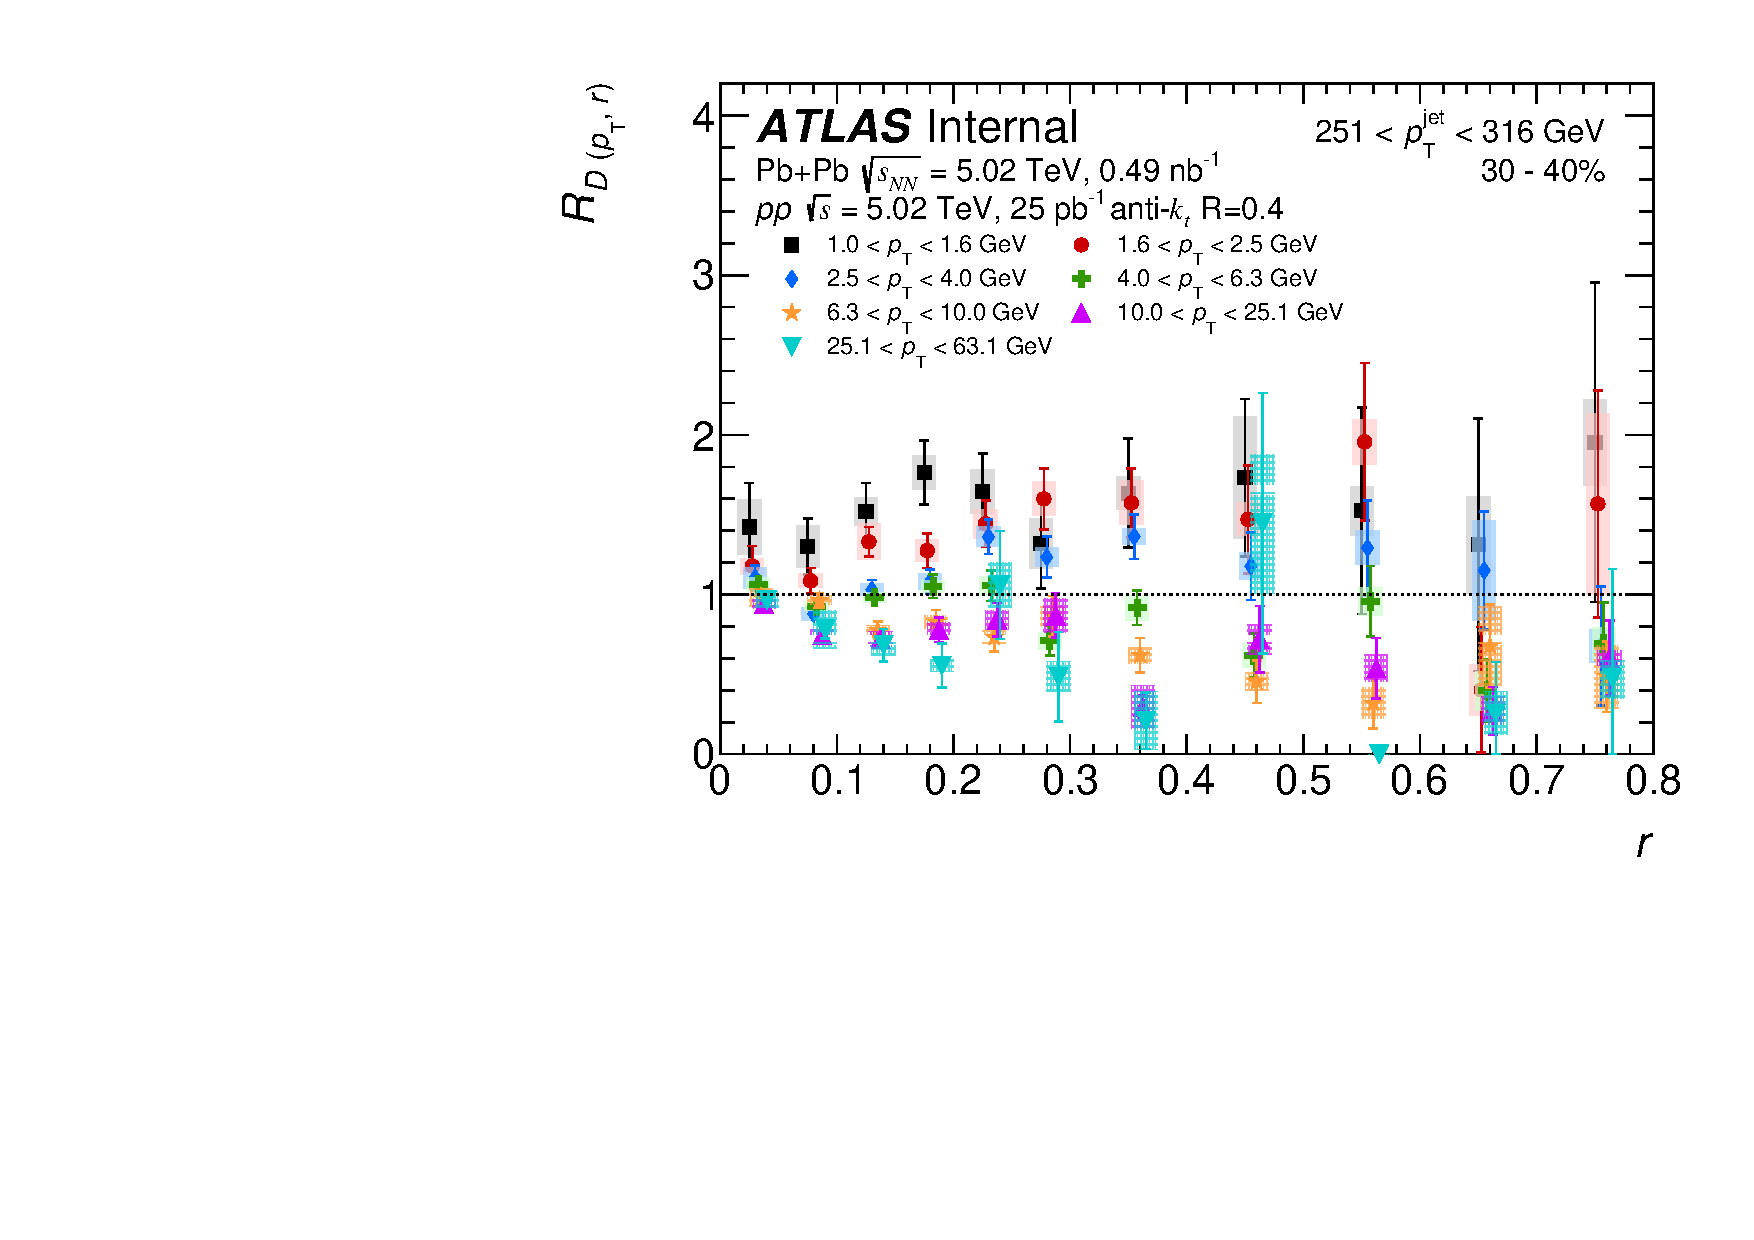
\includegraphics[width=0.48\textwidth]{figures/results/RDpT_dR_jet10_cent3} \\
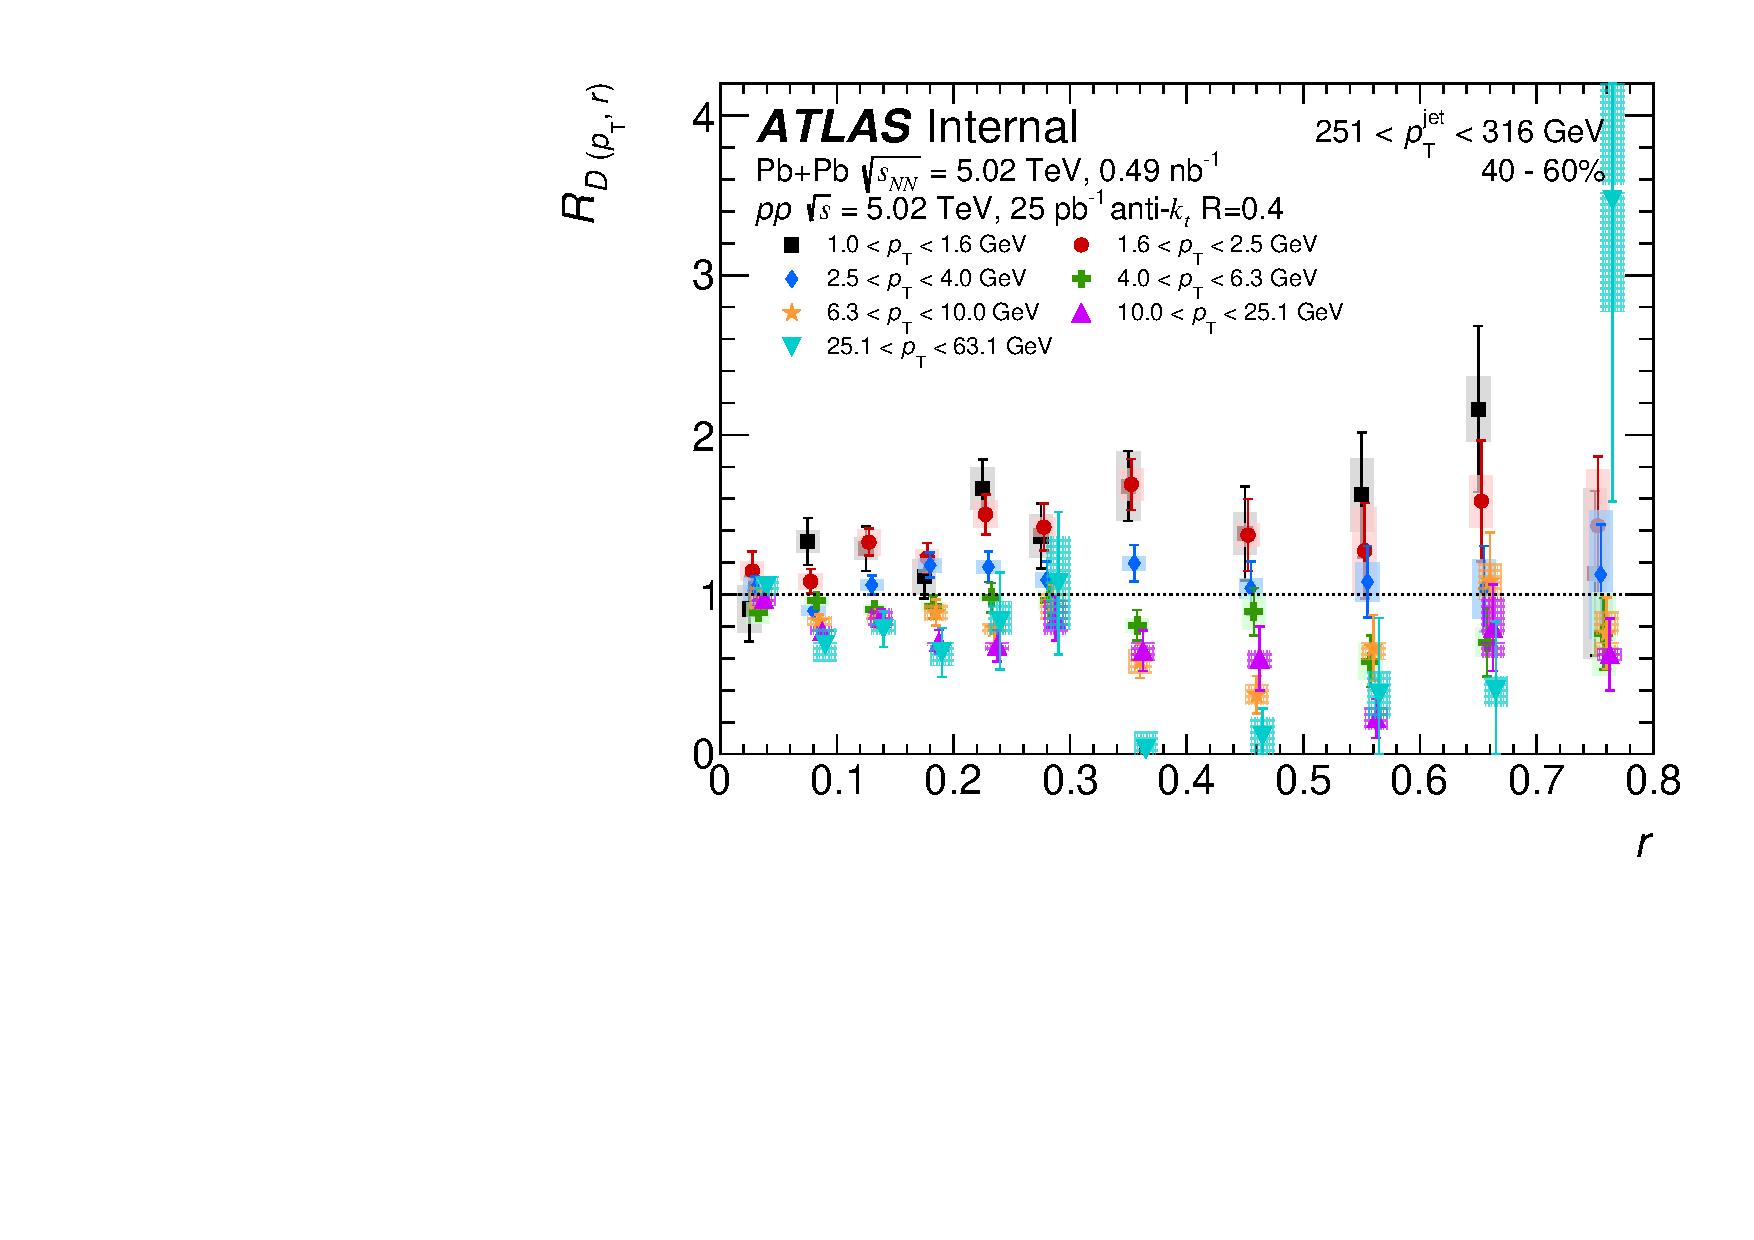
\includegraphics[width=0.48\textwidth]{figures/results/RDpT_dR_jet10_cent4} &
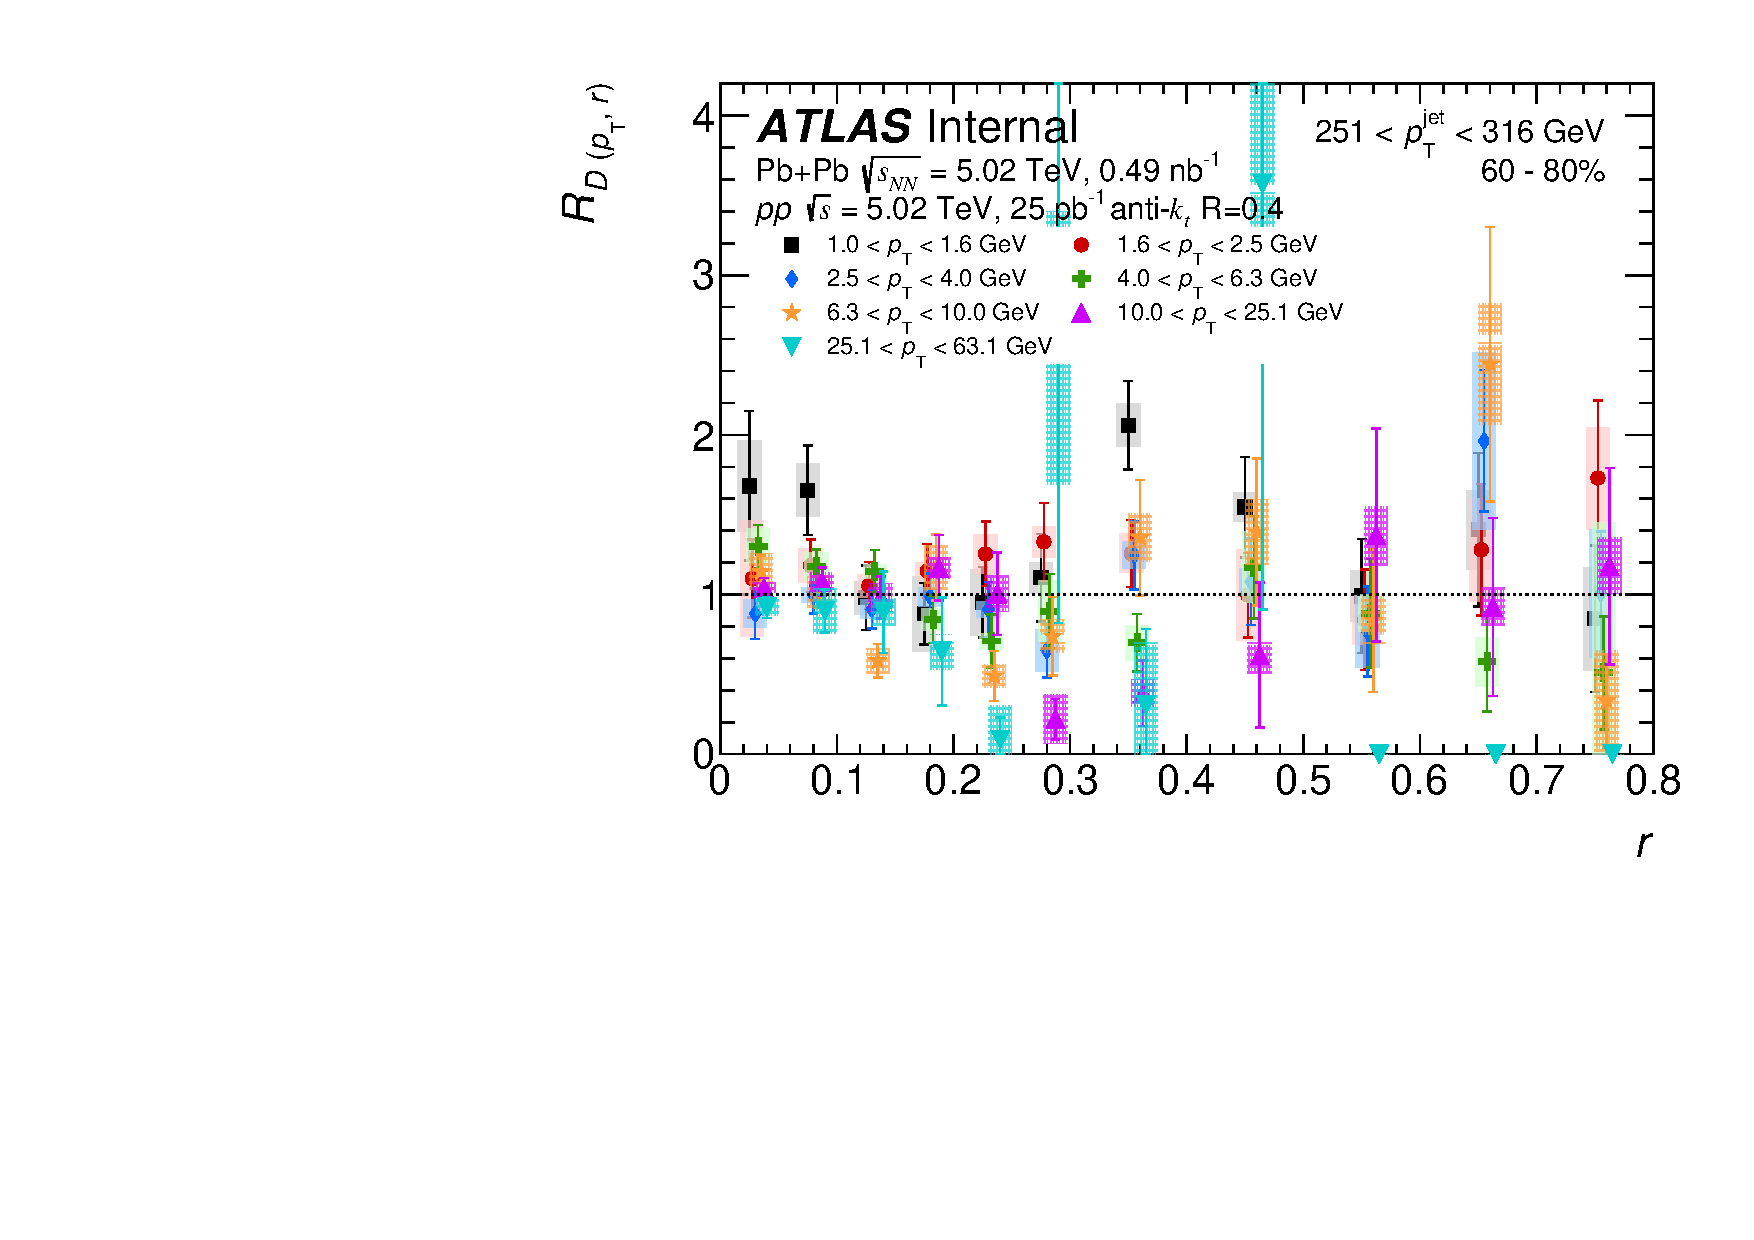
\includegraphics[width=0.48\textwidth]{figures/results/RDpT_dR_jet10_cent5} \\
\end{tabular}}
\caption{ The \RDptr\ distributions as a function of \rvar\ for different \pt\ selections in 251--316 GeV jets.
The different panels refer to different centrality selections.
The vertical bars on the data points indicate statistical uncertainties while the shaded boxes indicate systematic uncertainties.
The widths of the boxes are not indicative of the bin size and the points are shifted horizontally for better visibility.}
\label{fig:fullset_rptr_j10}
\end{figure}
